\documentclass[10.5pt, openright]{book} %Document type 
\raggedbottom


%\bibliography{library.bib}
\usepackage{graphicx} % Required for inserting images
\graphicspath{ {./images/} }
\usepackage{caption}
\captionsetup{font=small, singlelinecheck=false, justification=justified}
\captionsetup[figure]{labelsep=period}
\captionsetup[table]{labelsep=period}
\usepackage{subcaption}
% \usepackage[backend=biber,sorting=nyt,style=apa, refsection=chapter, natbib]{biblatex}
\usepackage[semicolon,round,sectionbib]{natbib}  %%%%Changed
\usepackage{chapterbib}    %%%%Changed

\usepackage[T1]{fontenc}
\usepackage{titlesec, blindtext, color}
\definecolor{gray75}{gray}{0.75}
\newcommand{\hsp}{\hspace{20pt}}
\titleformat{\chapter}[hang]{\Huge\bfseries}{\thechapter\hsp\textcolor{gray75}{|}\hsp}{0pt}{\Huge\bfseries}


% \renewcommand*{\bibfont}{\fontsize{10}{12}\selectfont}

% add your references to this file
%\addbibresource{Library_test.bib}
%\addbibresource{refs_intro.bib}
%\addbibresource{refs_ch2.bib}
%\addbibresource{refs_ch3.bib}
%\addbibresource{refs_ch4.bib}
%\addbibresource{refs_ch5.bib}
%\addbibresource{refs_disc.bib}

% \bibliography{Ch2_bibtex, Ch3_bibtex,Ch4_bibtex,Ch5_bibtex,ChDisc_bibtex,ChIntr_bibtex}

\usepackage{subfig}
\usepackage{tabto} %to add tabs
\usepackage{setspace} %to change spacing between lines
\usepackage{titlesec}
\usepackage{ragged2e} %to center text of flush them to the left or right side
%\justifying

\usepackage{hyphenat}

%\graphicspath{ {images/} }
\usepackage{fourier-otf} %same
\usepackage{array}
\usepackage{makecell}
\usepackage{booktabs} %for table lines 
\usepackage{tabularx}
% \usepackage[b5paper,margin=1in]
%\usepackage{CJKutf8} % for chinese text
% \usepackage[utf8]{inputenc}
\usepackage{xeCJK} % for chinese text
% \setCJKmainfont{Noto Sans Traditional Chinese}
% \usepackage{microtype}
% \usepackage[b5paper, inner=1.25in, outer=1in, top=1in, bottom=1in]{geometry}

\usepackage[b5paper, inner=1in, outer=0.75in, top=1in, bottom=1in]{geometry}

\geometry{papersize={17cm,24cm}}
\usepackage{float}
\usepackage{fancyhdr}
\usepackage{wrapfig}
\pagestyle{fancyplain}% <- use fancyplain instead fancy
\usepackage{longtable}
\usepackage{xltabular} % for long tables
\usepackage{tabularray}
\usepackage{multirow}
\usepackage[table]{xcolor}
\usepackage{tipa}
\usepackage{longtable}
% \usepackage{floatrow}%for getting images next to text
\usepackage{boldline} %for bold lines in tables
\usepackage{xcolor}
\usepackage{ltablex}
\usepackage{framed, multido}
\usepackage{eso-pic} %for adding background
\usepackage[absolute]{textpos}
\usepackage{rotating} %for rotating figures

%_______ Setting Font ____________________________________
% \usepackage[T1]{fontenc}
% \usepackage{lmodern}
% \renewcommand{\familydefault}{lmss}

\usepackage{fontspec}
\setmainfont{Palatino Linotype}
%___________________________________________

\usepackage{tabularx,ragged2e,booktabs,caption}
\newcolumntype{C}[1]{>{\Centering}m{#1}}
\renewcommand\tabularxcolumn[1]{C{#1}}

\usepackage{pdflscape} %for changing the tables 90 degrees
\usepackage{afterpage} %same



%\usepackage[colorinlistoftodos]{todonotes}
%\usepackage{listings}
%\usepackage[ruled,vlined]{algorithm2e}
%\usepackage{xcolor}
%\usepackage{rotating}
%\usepackage{amsmath}
%\usepackage[letterpaper,top=2cm,bottom=2cm,left=3cm,right=3cm,marginparwidth=1.75cm]{geometry} %Changing the margins
    %Margin options are: a0paper, a1paper, a2paper, a3paper, a4paper, a5paper, a6paper,b0paper, b1paper, b2paper, b3paper, b4paper, b5paper, b6paper,c0paper, c1paper, c2paper, c3paper, c4paper, c5paper, c6paper,b0j, b1j, b2j, b3j, b4j, b5j, b6j,ansiapaper, ansibpaper, ansicpaper, ansidpaper, ansiepaper,letterpaper, executivepaper, legalpaper
%\usepackage{includeenc}
%\usepackage{csquotes}


%\usepackage[demo]{graphicx}
%\usepackage[some]{background}

\usepackage{lipsum}
% \usepackage{showframe}
\usepackage{tikz}
\usepackage{xstring}

% \AddEverypageHook{\AddLogoIfCurrentPageIsOnList}%




% \newcommand{\MyGraphicLogofour}{% For imported graphic logo
% \begin{tikzpicture}[remember picture,overlay,yshift=-2cm, xshift=2cm]
%   \node at (9,-25) {\includegraphics[width=1cm,height=1cm]{Figures/test_logo2.jpg}}; %write the name of the image
%  \end{tikzpicture}
% }

% \SetBgContents{\MyGraphicLogofour}% Select included image

% \SetBgPosition{current page.north west}% Select location
% \SetBgOpacity{1.0}% Select opacity
% \SetBgAngle{0.0}% Select roation of logo

% \SetBgScale{1.0}% Select scale factor of logo

% \newcommand*{\ListOfPagesWithLogofour}{2,...,62}% %need to write the last page number 

% \makeatletter
% \newcommand*{\AddLogoIfCurrentPageIsOnLisfour}{%
%     \foreach \LogoPage in \ListOfPagesWithLogofour {%
%         \IfEq{\arabic{page}}{\LogoPage}{%
%             \bg@material%
%             \breakforeach%
%         }{}%
%     }%
% }%
% \makeatother
% \AddEverypageHook{\AddLogoIfCurrentPageIsOnLisfour}%
\usepackage{titletoc}% http://ctan.org/pkg/titletoc

% \titlecontents*{chapter}% <section-type>
%   [0pt]% <left>
%   {}% <above-code>
%   {\bfseries\chaptername\ \thecontentslabel\quad}% <numbered-entry-format>
%   {}% <numberless-entry-format>
%   {\bfseries\hfill\contentspage}% <filler-page-format>

\usepackage{tocloft,calc}


%---------------add thumb index------------

% % background common settings
% \usepackage[
%   scale=1,
%   angle=0,
%   opacity=1,
%   contents={}
% ]{background}
% \usetikzlibrary{calc}
% \usepackage{lipsum}

 \pagestyle{plain}

% % auxiliary counter
% \newcounter{chapshift}
% \addtocounter{chapshift}{-1}

% % the list of colors to be used (add more if needed)
% \newcommand\BoxColor{red!40}

% % the main command; the mandatory argument sets the color of the vertical box
% \newcommand\ChapFrame{%
%     \AddEverypageHook{%
%     \ifnum\value{page} < 8
%     \else  
%         \ifnum\value{page} = 29
%         \else
%             \ifnum\value{page} = 63
%             \else
%                 \ifnum\value{page} = 103
%                 \else
%                     \ifnum\value{page} = 147
%                     \else
%                         \ifnum\value{page} = 189
%                         \else
%                             \ifnum\value{page} = 215
%                             \else
%                                 \ifnum\value{page}= 263
%                                 \else
%                                 \ifodd\value{page}
%                                   \backgroundsetup{contents={%
%                                     \begin{tikzpicture}[overlay,remember picture]
%                                       \node[
%                                         fill=\BoxColor,
%                                         inner sep=0pt,
%                                         rectangle,
%                                         text width=1cm,
%                                         text height=2.5cm,
%                                         align=center,
%                                         anchor=north east
%                                       ] 
%                                       at ($ (current page.north east) + (-0cm,-2*\thechapshift cm -3.5cm) $) 
%                                       {\rotatebox{90}{\hspace*{.3cm}\parbox[c][0.3cm][t]{1.9cm}{%
%                                           \raggedright\textcolor{black}{\scshape\leftmark}}}};
%                                     \end{tikzpicture}%
%                                   }%
%                                 }  
%                                 \else
%                                   \backgroundsetup{contents={%
%                                     \begin{tikzpicture}[overlay,remember picture]
%                                     \node[
%                                       fill=\BoxColor,
%                                       inner sep=0pt,
%                                       rectangle,
%                                       text width=1cm,
%                                       text height=2.5cm,
%                                       align=center,
%                                       anchor=north west
%                                     ] 
%                                     at ($ (current page.north west) + (-0cm,-2*\thechapshift cm-3.5cm) $) 
%                                     {\rotatebox{90}{\hspace*{0.25cm}\parbox[c][0.3cm][t]{2cm}{%
%                                         \raggedright\textcolor{black}{\scshape\leftmark}}}};
%                                     \end{tikzpicture}%
%                                   }%
%                                 }
%                                 \fi
%                             \fi 
%                         \fi 
%                     \fi 
%                 \fi
%             \fi
%         \fi
%     \fi
%     \fi
%   \BgMaterial}%
%   \stepcounter{chapshift}%
% }

% % redefinition of \chaptermark to contain only the title
% \renewcommand\chaptermark[1]{\markboth{{\fontfamily{lmss}\selectfont Chapter \thechapter}}{}} 

%-----------------------------------------------

\renewcommand{\cftchappresnum}{Chapter }
\AtBeginDocument{\addtolength\cftchapnumwidth{\widthof{\bfseries Chapter }}}


% \cftsetindents{section}{2em}{3em}
\usepackage{tocloft}
% \setlength{\cftchapterindent}{4em}
\cftsetindents{chapter}{0em}{4em}
% \renewcommand{\@tocrmarg}{6em}
\renewcommand{\contentsname}{\LARGE Table of Contents}

\makeatletter
\renewcommand\@tocrmarg{0.5in}
% \renewcommand*\l@chapter{\@dottedtocline{0}{1.5em}{4em}}
\makeatother
% \setlength{\cftsetindent}{section}{4em}

%----------------------------------------------------------

% \usepackage{tcolorbox}
%https://osl.ugr.es/CTAN/macros/latex/contrib/tcolorbox/tcolorbox.pdf

\usepackage{fancybox}

% \tcbuselibrary{breakable}
% \tcbset{%any default parameters
%   width=0.9\textwidth,
%   halign=justify,
%   center,
%   breakable,
%   colback=white    
% }

% \usepackage{hyperref} % Add the hyperref package to enable hyperlinks

\usepackage{xcolor}
\definecolor{navy}{HTML}{102573}

\usepackage[
  colorlinks=true,
  linkcolor=navy,
  urlcolor=navy,
  citecolor=navy
]{hyperref}

% \hypersetup{
%     hidelinks
% }


\begin{document}


\frenchspacing
\doublespacing
\pagenumbering{arabic}

\setcounter{secnumdepth}{0}
%\pagestyle{fancy}

\titleformat{\chapter}[display]
  {\normalfont\LARGE\bfseries\raggedright\centering}{\chaptertitlename\ \thechapter}{0pt}{\LARGE}
\titlespacing*{\chapter}{0pt}{-50pt}{-50pt}
\titlespacing*{\section}{0pt}{*1}{*1}
\titlespacing*{\subsection}{0pt}{*1}{*1}

% Clear default headers and footers
% \fancyhead[LE]{\thumbindex} % Left (even) pages
%\pagestyle{fancy} % Apply the custom page style


% \maketitle

% \begin{titlepage}
%     \begin{center}
%     \vspace*{1cm}

%       \title{Nutrition's Route to Behaviour and Vice Versa:\\ Longitudinal Links from Early Life to Adolescence}
%       \date{}
%       \vfill
%       \author{Yvonne Willemsen}
%       \vfill
%     \end{center}
% \end{titlepage}
\newpage
\thispagestyle{empty}
    \begin{tikzpicture}[remember picture, overlay]
      \node[inner sep=0] at (current page.center) {\includegraphics{Figures/cover_final.pdf}};
    \end{tikzpicture}

\newpage
\thispagestyle{empty}


\begin{titlepage}
   \AddToShipoutPictureBG*{%
  \AtPageLowerLeft{%
    \begin{tikzpicture}[remember picture, overlay]
      \node[inner sep=0] at (current page.center) {\includegraphics[width=\paperwidth, height=\paperheight]{Figures/cover_bg.pdf}};
    \end{tikzpicture}
}
}

\begin{Center}
\vspace{15cm}

{\fontsize{15}{14}\selectfont
\noindent \textbf{Heterogeneity maketh the mind: An exploration of electrical heterogeneity in cortical neurons}\\}

\vfill
Nishant Joshi\\
\end{Center}  


\newpage
\thispagestyle{empty}
\begin{spacing}{1.0}
\begin{figure}[h]
    % \hspace*{2cm} % Adjust the horizontal position of the entire figure
    % \vspace*{-1cm} % Adjust the vertical position of the entire figure
    % \centering
    \begin{subfigure}{0.1\linewidth}
        
\includegraphics[scale=0.12]{Figures/eu_flag.pdf}
    \end{subfigure}
    \hspace{1.5cm} % Adjust the horizontal space between the images
    \begin{subfigure}{0.1\linewidth}
        
\includegraphics[scale=0.3]{Figures/new-brain-nutrition_logo.pdf}
    \end{subfigure}
\end{figure}

\noindent This project has received funding from the European Union's Horizon 2020 
research and innovation program under the Marie Skłodowska-Curie grant agreement No 860949.
\vspace{0.7cm}

\noindent Author: Nishant Joshi
\newline \noindent Title: Heterogeneity maketh the mind: An exploration of electrical heterogeneity in cortical neurons
\vspace{0.7cm}

\newline \noindent Radboud Dissertations Series
ISSN: 
\vspace{0.7cm}

\newline \noindent Published by RADBOUD UNIVERSITY PRESS 
\newline \noindent Postbus 9100, 6500 HA Nijmegen, The Netherlands 
\newline \noindent www.radbouduniversitypress.nl 
\vspace{0.7cm}

\newline \noindent Design: Nishant Joshi
\newline \noindent Cover: TBD
\newline \noindent Printing: 
\vspace{0.7cm}

\noindent ISBN: 
\newline \noindent DOI: 
\newline \noindent Free download at: www.boekenbestellen.nl/radboud-university-press/dissertations
\vspace{0.7cm}

\newline \noindent © Nishant Joshi, 2025

\begin{figure}[h]

\includegraphics[scale=0.1]{Figures/rup.pdf}
\end{figure}


\begin{justify} 
\noindent This is an Open Access book published under the terms of Creative Commons Attribution-Noncommercial-NoDerivatives International license (CC BY-NC-ND 4.0). This license allows reusers to copy and distribute the material in any medium or format in unadapted form only, for noncommercial purposes only, and only so long as attribution is given to the creator, see http://creativecommons.org/licenses/by-nc-nd/4.0/. 
\end{justify}

\end{spacing}
  
\newpage
\thispagestyle{empty}
  \begin{center}
       \vspace*{0cm}
        
       \textbf{\Large Heterogeneity maketh the mind: An exploration of electrical heterogeneity in cortical neurons}\\
          
       \vspace{2cm}

       Proefschrift ter verkrijging van de graad van doctor\\
        aan de Radboud Universiteit Nijmegen \\
        op gezag van de rector magnificus prof. dr. J.M. Sanders,\\
        volgens besluit van het college voor promoties\\
        in het openbaar te verdedigen op\\

        \vspace{1cm}
        % maandag 15 april 2024\\
        % om 16:30 uur precies\\
        \vspace{1cm}
        door\\

        \vspace{1cm}
        
        Nishant Joshi\\
        geboren op 26 January 1994\\
        te Varanasi, India\\
       \vfill
     
       % \includegraphics[width=0.4\textwidth]{university}
            
       % Department Name\\
       % University Name\\
       % Country\\
       % Date
            
   \end{center}  
\end{titlepage}


\newpage
\thispagestyle{empty}
\noindent{\textbf{Promotor:}}
\newline{Prof. dr. T. Celikel}
\vspace{1cm}
\newline{\textbf{Copromotoren:}}
\newline{Dr. F. Zeldenrust}
\vspace{1cm}
\newline{\textbf{Manuscriptcommissie:}}
\newline{TBD.}
\newline{TBD.}
\newline{TBD.}
\newline{TBD.}
\newline{TBD.}

\newpage
\thispagestyle{empty}
\noindent{\textbf{Funding}} 
\newline{This project has received funding from the European Union's Horizon 2020 research and innovation program under the Marie Skłodowska-Curie grant agreement No 860949.}


\newpage\null\thispagestyle{empty}\newpage
\setcounter{tocdepth}{1}
\clearpage
\thispagestyle{empty}
\tableofcontents
\fancyhf{} 
\clearpage
\newpage


% \newpage 
% \titlepage


\chapter{General Introduction}
% \ChapFrame

 

% \AddToShipoutPictureBG*{%
%   \AtPageLowerLeft{%
%     \begin{tikzpicture}[remember picture, overlay]
%       \node[inner sep=0] at (current page.center) {\includegraphics[width=\paperwidth, height=\paperheight]{Figures/1.pdf}};
%     \end{tikzpicture}
%   }
% }

% \begin{tikzpicture}[remember picture, overlay]
%   \node[anchor=north, xshift=0.4cm, yshift=-4.5cm] at (current page.north)  {\includegraphics[scale=0.65]{Figures/cover_orb.png}};
% \end{tikzpicture}
\clearpage
\fancyhf{}
\fancyhead[c]{Chapter 1. General Introduction}% <- added
\fancyfoot[R]{\thepage\ifodd\value{page}\else\hfill\fi}
%\fancyhead[L]{\ifodd\value{page}\relax\else\hfill\fi Ch \thechapter}
%\renewcommand\headrulewidth{0pt}% default ist .4pt
\renewcommand{\plainheadrulewidth}{.4pt}% default is 0pt

\newpage

\noindent I urge you to look around you and observe the trees, the leaves on them, each one with a unique shape and size, isn't it? Look at the people surrounding you, how they have different skin colors, facial features, heights, voice and thoughts. Now take a look at your palm, go ahead and examine it. What do you see? Aren't all five of your fingers different from each other? If you look even closer, you'd see that even the scales and crevices on your fingers are not the same. Have you ever wondered why nothing is exactly the same? Variance is an essential feature of nature; it permeates everything, from our thoughts and dreams to our language and societies. Without this diversity, life would be sterile, perhaps even impossible.

In this thesis, I have sought to understand the origins and implications of these differences at the most 
fundamental level: the neurons inside our brains. By exploring the variability among these building blocks 
of thought, ideas, dreams, language, and personality, I aim to shed light on how diversity shapes not only 
our individual experiences but also the very fabric of life. Neuroscience has long treated neurons as discrete, static ‘cell types’. But accumulating evidence shows identity lies on a continuum, is context-dependent, and heterogeneous. My aim with this thesis is to demonstrate that neuronal identity, especially the functional identity is not static but is rather dependent on the context and level of receptor specific neuromodualtion.  


\section{Neuronal heterogeneity through the lens of the past}

The mammalian brain is an extraordinarily complex organ, composed of an immense variety of neuronal cell types. This diversity is evident across multiple dimensions. Exploring this diversity has been a central tenet in neuroscience, since its inception, dating back to Ramon y Cajal (\cite{fishell2013neuron, huang2019diversity, markram2004interneurons, mukamel2019perspectives, nelson2006problem, petilla2008petilla, sanes2015types, seung2014neuronal, somogyi2005defined, yuste2020community, zeng2022cell, zeng2017neuronal}). I would like to take the reader through what we already know about neuronal heterogeneity via different modalities, 
ranging from shapes to molecular composition.    

\subsection{Morphology}

Neurons differ dramatically in their shapes and structures. Some, like pyramidal neurons, exhibit long 
apical dendrites and a characteristic triangular soma, while others, such as inter-neurons, display 
more compact and intricate branching patterns. These morphological differences are closely linked to 
the specific roles neurons play within neural circuits (\cite{liu2024neuronal}).


\subsection{Electrophysiology}

Neuronal diversity is also exhibited in the ways neurons generate and propagate electrical signals. 
Neurons exhibit distinct firing patterns, action potential shapes, spike frequency adaptation and selectivity to synaptic input. For instance, some neurons are fast-spiking, while others display spike frequency adaptation or bursting firing patterns. These electrophysiological properties are determined by the unique composition of ion channels and receptors expressed by each neuron (\cite{huang2019diversity, markram2004interneurons, mukamel2019perspectives, fishell2013neuron, masland2012neuronal, tasic2018shared, zeng2017neuronal}).


\subsection{Gene Expression}

Advances in molecular biology have revealed that neurons can be distinguished by their gene expression profiles. Single-cell RNA sequencing has enabled researchers to catalog the transcriptomes of individual neurons, uncovering a rich landscape of molecular identities. These profiles often correlate with, but are not strictly determined by, morphological and electrophysiological features (\cite{wagner2016revealing, shapiro2013single, trapnell2015defining}).


\subsection{Connectivity}

Neurons are further defined by their patterns of connectivity, both the sources of their inputs and the targets of their outputs. Some neurons form long-range projections across brain regions, while others 
participate in local microcircuits. This connectivity further defines the broader neural circuit function. (\cite{Wang2021, Zhang2024, Gollo2020, Goldman2023, Tripathy2017, Sagner2019} )

These modalities highlight the fact that neuronal heterogeneity is multi-faceted, and challenges the notion of n-neuron types. There have been many integrative efforts that merge these different modalities. 

\subsection{Cataloging neuronal heterogeneity}

In the following section we highlight the large scale efforts to study neuronal heterogeneity based on different modalities as well as the efforts towards integrating these individual modalities into a complete taxonomic picture of neuronal heterogeneity in the brain. 

\subsection{Large-Scale Taxonomy Initiatives}

In the past decade, large-scale collaborative efforts have sought to systematically map and classify the full 
diversity of neurons in the brain. Notable among these are the Allen Institute for Brain Science's Cell Types 
Program and the BRAIN Initiative Cell Census Network (BICCN). These projects leverage cutting-edge techniques, including high-throughput single-cell transcriptomics, large-scale electrophysiological recordings, and high-resolution imaging to build comprehensive taxonomies of neuronal types \cite{gouwens2019classification,gouwens2020integrated}.

While these initiatives have greatly expanded our understanding of neuronal diversity, they often operate under the assumption that neuronal identity is static and can be captured by a fixed set of features. However, emerging evidence suggests that neuronal identity may be more dynamic and context-dependent than previously thought, raising important questions about how best to define and classify the brain's myriad cell types.

\subsection{Patch-seq}

The state of the art in recording neuronal data is a technique known as patch-seq (\cite{cadwell2016electrophysiological, fuzik2016integration}), whereby it is possible to simultaneously record morphological, electrophysiological and molecular properties of neurons. This technique is really powerful as it provides a multi-modal perspective on neuronal heterogeneity. This technique has been the linchpin in some of the biggest classification efforts such as by the Allen Brain database (\cite{gouwens2019classification, gouwens2020integrated}), with a multi-modal collection of more than 1900 neurons. 

\section{Classification }

So far we have established that neuronal heterogeneity is multi-modal and the amount of data is growing exponentially. In order to leverage this growth in data and multi-modal picture, it becomes apparent to categorize neurons based on their similar characteristics. In the following sections we will look at some of the classification approaches and discuss their limitations.  

\subsection{Traditional Classification Approaches}

Historically, neuroscientists have sought to classify neurons into discrete “types” based on intrinsic, 
relatively stable characteristics. Early classification schemes focused on observable features such as 
soma size, dendritic arborization, and axonal projections. With the advent of intracellular recording techniques, electrophysiological properties like spike shape, firing rate, and synaptic integration became central to neuronal taxonomy. More recently, molecular markers such as the expression of specific neurotransmitters, calcium-binding proteins, or transcription factors have been used to further refine neuronal classifications.

The underlying assumption in many of these approaches is that each neuron possesses a fixed identity: a stable set of features that persists across time and context. This has led to the widespread use of terms like 
''cell type'' and ''canonical neuron'', suggesting a degree of invariance in neuronal identity.

Here I challenge this classic view by testing if neuronal classification depends on the external factors such the somatic input distribution and neuromodulation. I have identified several limitations to this assumptions which involve the the way neurons interact with the network in which they are embedded and the recordings protocols. In the next section I am going to highlight the most pressing limitations which establish that the idea of static neuronal identity needs a revision.  


\subsection{Limitations of Static Neuronal Classification}

In this section we discuss some of the limitations of a static neuronal classification. For a long time neuronal function has been discussed in the field of neuroscience as invariant. This is apparent with the input protocol used to study function of neurons. For example, since the beginning of single unit patch-clamp recordings, a static step input has been used to probe the firing rates of neurons. The following points challenge this view by highlighting problems with this assumption: 

\begin{itemize}

    \item  \textbf{The Influence of Input and Network State on Neuronal Function} Recent experimental and computational efforts have increasingly pointed towards the idea that a neuron's functional role is not solely determined by its intrinsic static properties such as morphology, gene expression, or ion channel 
dynamics but also by the nature of the input it receives and its dynamic state within a circuit (\cite{hernath2019alternative,szabo2021conventional}). Neurons operate within continuously changing environments, receiving temporally structured synaptic input that reflects sensory stimuli, behavioral 
demands, and ongoing internal activity. These inputs interact with intrinsic biophysical parameters in 
complex ways, such that the same neuron may perform different computational roles depending on the input regime or network context. Additionally, neuromodulatory systems (e.g., dopaminergic and cholinergic pathways) further reconfigure neuronal function in a cell-type- and receptor-specific manner, modulating excitability, gain, adaptation, and stimulus selectivity. This context-dependence challenges the classical view of neurons as fixed computational units. 
    
    \item \textbf{Continuous neuronal identity}
Recent large scale neuronal classification efforts have consistently shown that neurons are not discrete 
modular classes but rather that their electrophysiological, molecular and morphological properties lie on a 
continuum \cite{marsat2010neural,angelo2012biophysical,scala2021phenotypic}. This further complicates the effort of classifying neurons in classes. 

    \item \textbf{Limitations of Static Characterization Protocols} Conventional approaches to neuronal classification typically rely on static stimulation protocols, such as step-and-hold current injections, to derive electrophysiological signatures. While these protocols offer insights into baseline excitability and passive membrane properties, they do not capture the complex temporal filtering or nonlinear input-output transformations that neurons perform under more realistic, time-varying conditions. In naturalistic settings, 
neuronal input is dynamic, high-dimensional, and often stochastic features that are absent in traditional 
measurements. As a result, static protocols risk underestimating or mis-characterizing the functional capabilities of neurons, potentially leading to oversimplified or misleading classifications. This disconnect 
highlights the need for rich stimulus paradigms, such as temporally varying current or (dynamic clamp) conductance stimuli or in vivo recordings, that better approximate the computational demands faced by neurons in situ.

    \item \textbf{Neuronal Identity as an Emergent, Dynamic Construct} Taken together, these observations point 
toward a new conceptual framework in which neuronal identity is not a fixed property, but rather a 
context-sensitive, emergent phenomenon. If neuronal function can be reshaped by synaptic input, neuromodulatory state, and network dynamics, then neuronal identity must be understood as fluid and multidimensional, rather than static and categorical. This dynamic view aligns with recent findings showing that neurons shift their classification depending on the input stimulus or modulatory condition. It also suggests that functional heterogeneity in neural populations is not simply biological variability, but may reflect adaptive specialization to a range of computational roles. 

In this thesis, I explore this emergent view by analyzing how neurons reorganize their functional attributes 
under different input regimes and neuromodulatory conditions, using high-dimensional clustering and 
integrative analysis across multiple feature domains. This work contributes to a growing shift in neuroscience: from static taxonomies to dynamic, functionally grounded models of neuronal identity. 
    
    \item \textbf{Rich high-dimensional functional space remains unexplored} The functional space of neurons is high 
dimensional, this is due to the fact activity of neurons depends on the activation/inactivation of ion multiple ion-channels (\cite{fyon2024dimensionality}), this can be summarized by passive properties such as resistance, capacitance, etc. Furthermore, neurons can filter inputs in temporal and spacial dimensions which further adds to the dimensionality (\cite{y2003computation}). But most electrophysiological classifications only consider one feature at a time. This leads to an incomplete picture of functional heterogeneity.  As we have discussed before, stimulus protocols have a strong role to play in features that can actually be extracted. For example a static step and hold input protocol doesn't expose the subthreshold potential dynamics of a neuron. Similarly, properties related to action potential are a function of the input protocol. Clustering based on these features typically involves looking at a low dimensional (1-3 dimensions) feature space using a method such as K-means clustering. This approach underestimates the rich functional space in which neurons function and thus clustering based on functional properties needs a method that utilizes multiple features pertaining to function simultaneously and provides a rich overview of functional heterogeneity. 
    
    \item   \textbf{No consensus on properties that are the most informative about heterogeneity} While neurons have been categorized based active and passive features there is no consensus on properties or a set of properties that are the most informative about heterogeneity. While most classification studies focus on passive properties such as capacitance or conductance of the cell or active properties such as firing rates and inter-spike intervals, there are no studies that compare the estimate of neuronal heterogeneity based on different sets of properties and provide a consensus for the field. Moreover, the properties extracted are limited by the stimulation protocol. For example it is not possible to estimate the linear input-filter of a neuron via a step input protocol, and thus it requires a white noise based stimulation protocol. Therefore, we must first establish the input protocol that is most suitable for studying a neuronal population and then compare properties extracted in each protocol to provide a consensus.  
\end{itemize}

The limitations listed above show that assuming a static neuronal identity is restrictive, it gives an incomplete picture of a rich high-dimensional and dynamic functional space in which neurons reside. Therefore a new method is required to ascertain the high dimensional and dynamic nature of neuronal function by taking into account the input context and functional properties used to study function. 

So far we have highlighted the limitations of input protocol and the lack of consensus in determining the most informative properties to study functional heterogeneity, but a very important still remains to be discussed and that is neuromodulation. Neurons consist of ion-channels that are susceptible to modulation via specific receptor activation molecules. These neuromodulators have a strong effect on the activity of neurons, they can suppress or enhance firing of a neuron. Therefore it is important to study how neuromodulation affects neuronal function and classification. The following section discusses the current state of understanding in terms of neuromodulation.   

\section{Neuromodulation: Reconfiguring Neural Computation}

Neuromodulatory systems, particularly those involving dopamine and acetylcholine play a critical role in shaping brain states associated with attention, learning, memory, and pathology. Rather than directly triggering spikes, these modulators reshape how neurons respond to input, modulating intrinsic excitability and synaptic integration. Their effects are often receptor and cell-type-specific, suggesting a finely tuned mechanism for reconfiguring the computational landscape of cortical networks.

Despite extensive behavioral and molecular work (\cite{nadim2014neuromodulation,mccormick2020neuromodulation,avery2017neuromodulatory}), the functional impact of neuromodulation on neuronal computation remains poorly understood, especially at the level of high-dimensional feature interactions. Are neuromodulatory effects isolated to individual electrophysiological features, or do they act in a coordinated manner to restructure how neurons encode information?

The following points summarize the gaps of what remains to be understood in regards to the effect of neuromodulation, specifically Dopaminergic and Cholinergic modulation, on single neurons: 

\begin{itemize}
    \item \textbf{Effect of neuromodulation on computation} Much is known \cite{dalley2004cortical,hasselmo2006cholinergic,sarter2009phasic,nusser2009variability} about molecular and excitability changes caused by dopamine and acetylcholine modulation in single neurons. Though it is still unclear how this alteration in excitability changes what neurons compute. Since neurons relay information within a network, it is unclear how dopamine and acetylcholine changes information transfer in neurons. Since activity of individual neurons determine that state of a network, it is clear that understanding alteration in transferred information due to neuromodulation would explain a lot about how cortical circuits are modulated. 

    \item \textbf{Heterogeneous modulation in neuronal population} A given population of neuron comprises of individuals or sub-groups of neurons that differ from each other in terms of their shape and and ion-channel type and distribution. It is still unclear how this individual variability manifests itself on a circuit scale. While it is known that this heterogeneity provides flexibility to  the circuit (\cite{wu2025neural,hutt2023intrinsic}), the effect of neuromodulation on this individuality is still unclear. More precisely, it is unknown if all functional properties are altered uniformly or if there exists a heterogeneity in terms of properties that are altered due to specific modulation and what are population level effects of neuromodulation. 

    \item \textbf{Reconfiguration under the influence of dopamine and acetylcholine} Most studies that focus on neuromodulation of individual neurons, focus on how individual active or passive properties such as firing rate or conductance are altered due to a specific receptor activation. While it is important to study how individual properties are altered due to neuromodulation, it is also important to study how the high-dimensional functional space of neurons is altered due to neuromodulation. This requires looking at correlation structure between active and passive properties of neurons and how this correlation structure changes due to neuromodulation.
\end{itemize}

So far we have looked at established view on neuronal heterogeneity, limitations of static neuronal classification, the effect of neuromodualtion on reconfiguring neuronal computation. Although much is known about heterogeneity in neural systems, it is still not completely understood how this intrinsic heterogeneity affect network function. In this next section we set the context for studying heterogeneity in an artificial network.  
          
\section{Effect of Temporal Heterogeneity in Artificial Systems}

Biological neural systems are composed of heterogeneous computational units (individual neurons) with diverse intrinsic properties (\cite{koch1999complexity}). This diversity has been shown to support critical functions such as motor control (\cite{cavanagh2020diversity}) and memory formation (\cite{mcnaughton2006path, hasson2008hierarchical, chu2020long}). While this fact is well-accepted in neuroscience, most artificial neural networks continue to be designed with homogeneous units.

Recurrent Neural Networks (RNNs), which possess temporal memory, have been proposed as functional analogs to biological circuits (\cite{sussillo2014neural}). One popular subclass, Reservoir Computing (RC) networks, or Echo State Networks (ESNs), have been demonstrated to have the capacity to solve tasks requiring short-term memory (\cite{jaeger2001echo}). However, these networks are typically built with uniform time constants and lack the diversity observed in biological systems.

Recent studies have introduced architectural temporal heterogeneity through mechanisms like delay lines. In particular, Distance-based Delay Networks (DDNs) have been shown to outperform classical ESNs on memory and chaotic time-series tasks (\cite{iacob2022distance, soriano2014delay}). Previous studies have also shown benefits of intrinsic heterogeneity in spiking network, more specifically on encoding and memory task (\cite{gast2024neural,perez-nieves_neural_2021,chakraborty_heterogeneous_2022,zeldenrust_efficient_2021, mejias_optimal_2012,tripathy_intermediate_2013,landau_impact_2016,doty_heterogeneous_2021,duarte_leveraging_2019}). These results suggest that incorporating temporal diversity improves computational performance. However, in such models, heterogeneity is embedded in network-level topology, not in the intrinsic properties of individual units.

Thus, it remains unclear how intrinsic temporal heterogeneity such as variability in decay rates of individual units in the network or integration time constants across individual units influences network performance. This thesis explores this gap by systematically varying internal timescales within reservoir units, testing whether biologically inspired temporal diversity can enhance memory capacity and task performance in artificial networks.

\section{Research Objectives and Key Questions}
This thesis addresses three overarching questions:

\begin{enumerate}
  \item \textbf{How does input context influence functional classification of neurons?} \\
In Chapter 2, we demonstrate that neuronal identity is not static, but input-dependent, with classification outcomes varying significantly under dynamic (frozen noise) vs static (step-and-hold) stimuli. This challenges the notion of fixed electrophysiological types and highlights the role of stimulus structure in shaping neural function.

  \item \textbf{How does neuromodulation alter the functional landscape of neurons?} \\
In Chapter 3, we explore how activation of dopaminergic (D1-R, D2-R) and cholinergic (M1-R) receptors reconfigures information encoding, shifting the correlation stricture between feature domains. We show that neuromodulatory effects are highly cell-type and receptor-specific, modulating not just individual functional attributes but also their coordination.

  \item \textbf{Can intrinsic timescale heterogeneity improve performance and memory in reservoir computing systems?} \\
In Chapter 4, we go from data analysis to network level study of intrinsic heterogeneity, for this we design 4 different variants of ESNs and DDNs with varying levels of timescale heterogeneity and optimize them to perform NARMA-30 and Mackey-Glass benchmark tasks. We study the effect of the designed heterogeneity on task performance, stability, representation and memory capacity. We show that an intermediate level of heterogeneity is optimum for solving the two benchmark tasks, suggesting heterogeneity requirement is task dependent.     
  
\end{enumerate}


\section{Experimental Framework and Approach}

For answering the first two research questions stated above, this thesis utilizes single unit in-vitro recordings form the somatosensory cortex layer 2/3 (\cite{da2018databank}). These recordings were performed in tandem, first using a static step and hold input protocol followed by a frozen noise protocol (see Fig. \ref{fig:input_protocol}). Within each input protocol, neurons were first recorded in a vehicle control (artificial cerebral spinal fluid - aCSF) condition and a drug condition, where a specific receptor agonist is added to the bath and the recording is performed again. Sometimes multiple control and drug trials are recorded for a single neuron.   

\subsection{Input Protocols }
\begin{figure}
    \centering
    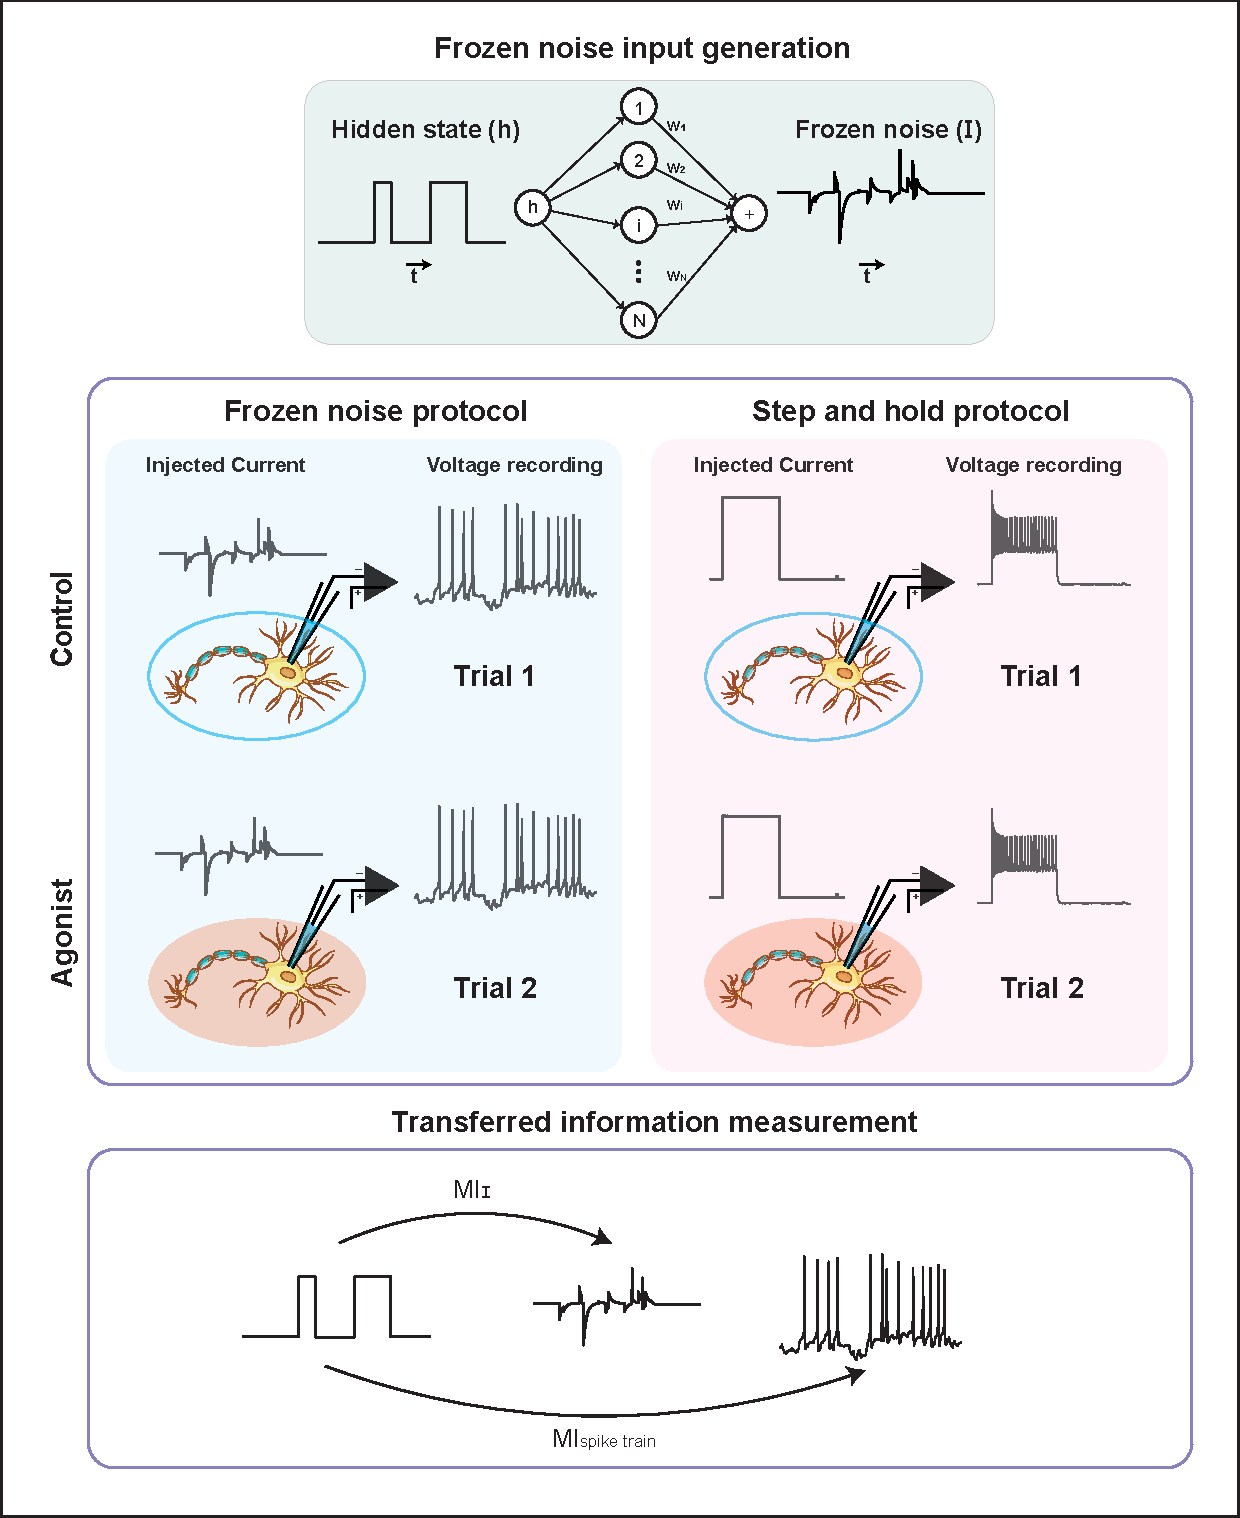
\includegraphics[width=\linewidth]{Figures/Intro/input_protocol.pdf}
    \caption{\textbf{Data collection and input protocol} the top figure shows the process of input generation using the hidden state and an artificial neural network. The middle figure shows the recording process, the neurons are recorded first in control condition using the frozen noise and step and hold inputs respectively, and then a specific receptor agonist is added, and the recording is repeated again. The bottom figure shows the procedure for measuring transferred information. Mutual information is measured between the hidden state and the input as well as between the hidden state and the spike train. } 
    \label{fig:input_protocol}
\end{figure}

\subsubsection{Step and Hold}

The step-and-hold protocol is a widely used electrophysiological method for characterizing neuronal properties through controlled current injections. In this protocol, a neuron's membrane potential is maintained at a baseline value (commonly around -70 mV), and then a series of incremental current steps are injected, each lasting for a fixed duration, typically 500 ms with recovery periods (e.g., 5.5 seconds) between steps. The current amplitude is increased in defined increments (e.g., 40 pA per step), allowing researchers to observe how the neuron responds to increasing levels of depolarizing input, including changes in firing rate, spike threshold, and other action potential characteristics. This approach enables the classification of neurons (such as distinguishing excitatory from inhibitory cells) and the assessment of properties like maximum firing frequency, spike latency, and after-hyperpolarization. The step-and-hold protocol thus provides a standardized way to probe intrinsic excitability and firing dynamics, serving as a foundational tool in cellular neurophysiology. 

\subsubsection{Frozen Noise}

The frozen noise protocol (\cite{zeldenrust2017estimating}), is a method designed to quantify the mutual information between a neuron's input and its spike train output in electrophysiological experiments. This protocol generates a time-varying input current by simulating the activity of a presynaptic neural network of 1,000 neurons, each firing Poisson spike trains in response to a binary "hidden state" (a Markov process representing the presence or absence of an external stimulus). 
The injected current is "frozen", meaning the same input sequence is used across trials or conditions, enabling a direct comparison of neuronal responses. By analyzing how the recorded neuron transforms this structured input into spikes, researchers can calculate the information-theoretic relationship between the hidden state and the output spike train. 
This approach overcomes limitations of traditional step-and-hold protocols by mimicking naturalistic synaptic input patterns while maintaining experimental control, allowing efficient bias-free information quantification with short (6 minutes) recordings. The protocol's output includes the injected current trace, hidden state time series, and the neuron's voltage response, facilitating both forward modeling of neuronal dynamics and reverse-engineering of coding principles. 

\subsection{Extracted features}
In order to provide a consensus about attributes sets that captures the highest amount of functional heterogeneity, we extracted neuronal function attributes categorized into four distinct attribute sets. The grouping is performed in order to capture distinct facets of neuronal function. This includes action potential shape and dynamics, passive properties associated with the physical aspect of neurons. The adaptation properties and the feature selectivity:

\begin{itemize}
  \item \textbf{Action Potential (AP) attributes} This set contains 22 features related to action potential shape and dynamics with their descriptive statics.  
  \item \textbf{Passive Biophysical (PB) attributes} This set contains 6 features related to passive properties such as membrane capacitance.   
  \item \textbf{Adaptation Currents (AC)} This attribute is a curve that captures the adaptation dynamic after an action potential.   
  \item \textbf{Input Feature Selectivity}, estimated using \textbf{Spike-Triggered Averages (STA)} This is an attribute that captures the input feature selectivity of neurons. 
\end{itemize}



An illustration of the feature extraction and analysis is shown in Fig. \ref{fig:feature_extraction}. To dissect the specificity and dynamics of neuronal encoding depending on input and neuromodulation, we apply unsupervised high-dimensional clustering (\cite{lee2021non}), cosine similarity analysis, and Multi-set Correlation and Factor Analysis (MCFA) (\cite{brown2023multiset}). This methods allow us to examine both within-attribute set variance and cross-attribute set coordination of attributes, offering a system-level view of functional reconfiguration.

\begin{figure}
    \centering
    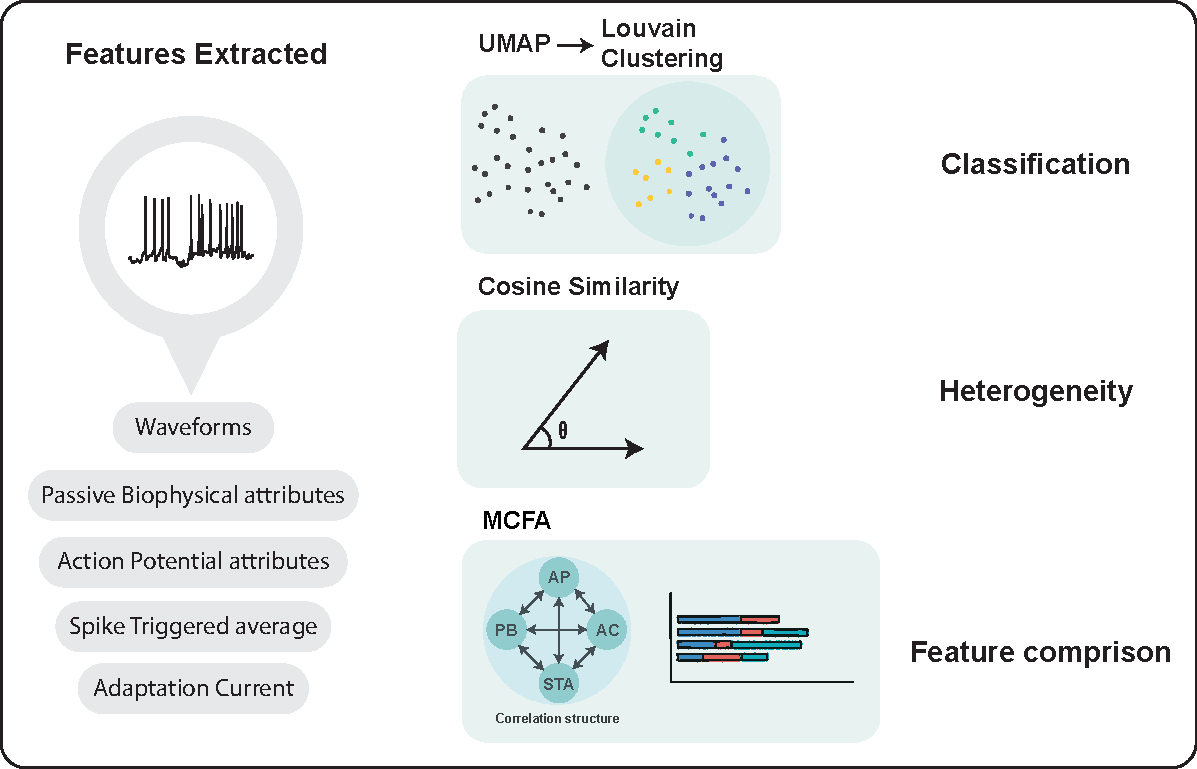
\includegraphics[width=\linewidth]{Figures/Intro/analysis_tools.pdf}
    \caption{\textbf{Overview of extracted features and analysis tools}}
    \label{fig:feature_extraction}
\end{figure}

\subsection{Network Design}
In order to study the effect of heterogeneity of intrinsic properties, in this case the time constant of individual units on computational properties of networks, we designed four different heterogeneity types for ESNs and DDNs, these configuration capture different levels of heterogeneity, we tested network wide heterogeneity and contrasted it with the network divided into clusters, with each cluster having its own parameter sampled from a distinct distribution. The designed network configurations are summarized as following: 
\begin{enumerate}
    \item \textbf{Homogeneous Network}: All units share a single decay (time constant) parameter.
    \item \textbf{Homogeneous Cluster}: The ESN/DDN is divided into clusters, each cluster with its own fixed decay parameter.
    \item \textbf{Heterogeneous Network}: Each unit samples its decay from a shared distribution.
    \item \textbf{Heterogeneous Cluster}: Each cluster samples decay parameters from different distributions.
\end{enumerate}

We also wanted to test if network heterogeneity is task dependent, which means if task complexity decides the requirement for the optimum level of network heterogeneity. We tested these networks on two benchmark tasks namely NARMA-30 and Mackey-Glass tasks:
\begin{itemize}
    \item \textbf{NARMA-30}: A nonlinear auto-regressive moving average task designed to test long-range memory and nonlinear dynamics. 
    \item \textbf{Mackey-Glass}: A chaotic time-series prediction task that evaluates a network's ability to generate stable yet complex temporal outputs.
\end{itemize} 

We aimed to train these designed ESNs and DDNs on the two tasks mentioned above and study the effect of intrinsic heterogeneity on stability, memory capacity and dimensionality of these networks. 

\section{Summary and Outlook}

This introduction has outlined the motivation and rationale for investigating neuronal identity and function through the dual lenses of input-dependence and neuromodulatory flexibility. Traditional classification approaches, though informative, fall short in capturing the high-dimensional, dynamic nature of neuronal computation. By leveraging state of the art patch clamp recordings done using frozen noise protocols, extracting high dimensional electrophysiological features from these recordings, and using modern unsupervised analysis techniques, this thesis proposes a data-driven framework to redefine neuronal identity as an emergent, context-sensitive construct. Finally, this thesis investigates the computational implications of intrinsic heterogeneity by modeling structured diversity in artificial reservoir systems. The following chapters present experimental results and theoretical insights that collectively support this paradigm shift.

\section{Thesis Structure}
\begin{itemize}
  \item \textbf{Chapter 2}: Neuronal Identity is Not Static: An Input-Driven Perspective \\
  Demonstrates how different stimulation protocols yield distinct classifications, showing that neuronal identity is dynamic and shaped by input.

  \item \textbf{Chapter 3}: Neuromodulatory Control of Cortical Function \\
  Examines how neuromodulators reshape the computational roles of neurons, altering both encoding capacity and feature interdependence.

  \item \textbf{Chapter 4}: Timescale heterogeneity in reservoir computing \\   
    Analyzes the effect of timescale heterogeneity on task performance of ESNs and DDNS, showing that moderate timescale heterogeneity improves the performance over networks without it.  

  \item \textbf{Chapter 5}: General Discussion and Future Directions \\
  Integrates findings across studies, discusses implications for neuroscience and artificial neural networks, and proposes directions for future research.
\end{itemize}


\newpage
\begin{spacing}{1.0} % Set the line spacing to single spacing
\fontsize{8pt}{8pt}\selectfont
\bibliographystyle{apalike}
\renewcommand{\bibname}{References}
\bibliography{All_bibtex}



\end{spacing}

%-------------------------------------------

\newpage
\chapter{Neuronal Identity is Not Static: An Input-Driven Perspective} 

\thispagestyle{empty}
\AddToShipoutPictureBG*{%
  \AtPageLowerLeft{%
    \begin{tikzpicture}[remember picture, overlay]
      \node[inner sep=0] at (current page.center) {\includegraphics[width=\paperwidth, height=\paperheight]{Figures/2.pdf}};
    \end{tikzpicture}
  }
}

% \begin{tikzpicture}[remember picture, overlay]
%   \node[anchor=north, xshift=0.4cm, yshift=-4.5cm] at (current page.north)  {\includegraphics[scale=0.65]{Figures/cover_line1.png}};
% \end{tikzpicture}
\vfill

\noindent Based on: \textbf{Joshi N}, van Der Burg S, Celikel T, Zeldenrust F (2025) Neuronal identity is not static: An input-driven perspective. PLoS Comput Biol 21(12): e1013821. \url{https://doi.org/10.1371/journal.pcbi.1013821} .

%\fancyhf{}
\fancyhead[c]{Chapter 2. Neuronal Identity is Not Static—An Input-Driven Perspective}% <- added
\fancyfoot[R]{\thepage\ifodd\value{page}\else\hfill\fi}
%\fancyhead[L]{\ifodd\value{page}\relax\else\hfill\fi Ch \thechapter}
%\renewcommand\headrulewidth{0pt}% default ist .4pt
\renewcommand{\plainheadrulewidth}{.4pt}% default is 0pt
%\fancyfoot[C]{\input{Figures/Test_logo.png}}
% \fancyfoot[C]{text works}

\newpage
\section{Abstract}
\tab Neuronal classification based on morphology, electrophysiology, and molecular markers is often considered static. Here, we challenge this view, showing that functional classification depends on input patterns. Using single-cell recordings from layer 2/3 barrel cortex neurons in mice, we compared responses to step-and-hold versus dynamic frozen noise inputs that mimic presynaptic activity. Action potential and waveform-based classifications varied significantly, highlighting the dynamic nature of neuronal identity. To assess the contribution of input versus neuronal attributes toward classification, we analyzed four attribute sets, namely action potential, passive biophysical, adaptation currents, and linear input filters derived via spike-triggered averages (STA). Our findings revealed that the STA, which captures a neuron’s selective responsiveness to presynaptic activity, explained the most variance within the population. This highlights input-driven dynamics as key to functional identity, emphasizing the need for physiologically relevant inputs in defining neuronal classes and shifting the focus from static properties to dynamic functional diversity.

\newpage

\section{Introduction}
\tab  Neural circuits are composed of diverse neuronal populations that exhibit variability in morphology, molecular composition, and electrophysiological properties. These neurons interact dynamically to process sensory information, support cognition, and drive behavior \cite{harris2015neocortical}. A long-standing challenge in neuroscience has been to classify neurons into meaningful functional groups, with traditional approaches relying on intrinsic features such as molecular markers, morphological characteristics, and electrophysiological properties. However, despite significant advances, a consensus on the most informative features for neuronal classification remains elusive \cite{huang2019diversity, markram2004interneurons, mukamel2019perspectives, fishell2013neuron, masland2012neuronal, tasic2018shared, zeng2017neuronal}. An often-overlooked dimension in this classification challenge is the role of input dynamics in shaping neuronal function.

Neurons act as spatiotemporal filters, transforming incoming synaptic inputs into output firing patterns. This transformation is governed by an interplay between the structure and dynamics of the input a neuron receives, and the intrinsic membrane processes this input dynamically recruits.. Traditional classification approaches, with a  focus on static properties, may therefore miss critical aspects of functional diversity that emerge from the interaction between neurons and their presynaptic partners. Recent studies suggest that electrophysiological identity is context-dependent \cite{gouwens2019classification, scala2021phenotypic, gouwens2020integrated}, varying as a function of the stimulation protocol used to probe neuronal function. However, a direct comparison of neuronal classification under physiologically realistic input conditions remains largely unexplored.


% \textbf{[Nishant: Here insert a summary of the relevant background information from your version]}


Recent advances in patch sequencing \cite{fuzik2016integration, cadwell2016electrophysiological, scala2019layer} enable simultaneous extraction of transcriptomic, morphological, and physiological properties, improving neuronal classification. The Allen Brain Institute dataset \cite{gouwens2019classification, scala2021phenotypic, gouwens2020integrated} provides a broad classification of visual and motor cortex neurons using multi-modal features (MET types). However, classification based on electrophysiology remains challenging. Neuronal properties exist on a continuum \cite{markram2004interneurons}, with unclear boundaries between classes. Moreover, molecularly defined types exhibit overlapping electrophysiological properties \cite{gouwens2019classification, gouwens2020integrated}, and intrinsic electrophysiology varies with stimulation protocols. While multi-modal techniques improve classification, they overlook the influence of synaptic input. Neurons receive inputs from thousands of presynaptic neurons shaping their firing properties, necessitating classification under physiologically realistic conditions \cite{connors1990intrinsic, steriade2000corticothalamic}.

 

To address this gap, we investigated how neuronal identity is shaped by the nature of the input a neuron receives. We recorded from layer 2/3 neurons in the barrel cortex and compared their responses under two different stimulation paradigms: a standard step-and-hold (SH) stimulus, which provides a static, artificial input, and a frozen noise (FN) stimulus \cite{zeldenrust2017estimating}, which simulates natural presynaptic activity. We hypothesized that functional classification of neurons would be stimulus-dependent, with the FN protocol revealing a distinct organization of neuronal diversity that is not captured by the SH protocol.

We analyzed four commonly used sets of electrophysiological attributes—action potential features, passive biophysical properties, adaptation currents, and linear input filters estimated via spike-triggered averaging (STA)—to assess their contributions to neuronal classification under dynamic input conditions. Using multiset  correlation and factor analysis, we found that the linear input filter, which characterizes a neuron’s sensitivity to specific input features, was the most informative attribute for understanding neuronal functional variance, i.e, it is the most relevant attribute to be used for clustering neurons. This finding challenges the traditional view that neuronal identity is a static property, emphasizing the importance of input dynamics on functional diversity.

By demonstrating that neuronal classification is highly dependent on input dynamics, our study highlights the need to incorporate physiologically relevant stimuli when defining neuronal types. Our findings suggest that neurons should not be categorized based solely on static features but rather on how they process and respond to dynamic synaptic input. This perspective has broad implications for both experimental and computational neuroscience, urging a paradigm shift toward input-dependent models of neuronal function.


\section{Materials and methods}

\textbf{Ethics statement} The data used in this research was previously published and made freely available to the community \cite{da2018databank} and \cite{yan2022whole}. All the experimental work, as outlined in the cited articles, were carried out in compliance with the European directive 2010/63/EU, the national regulations of the Netherlands, and international standards for animal care and use.    

\begin{flushleft}
\textbf{Slice electrophysiology} Data acquisition procedures, the details of the in vitro slice preparation, intracellular access to anatomically targeted neurons, data digitization, and preprocessing have been described in detail elsewhere \cite{kole2020assessing,kole2019neocortical,da2018databank,kole2017proteomic,miceli2017reduced}. In short, Pvalbtm1(cre)Arbr (RRID:MGI:5315557) or Ssttm2.1(cre)Zjh/J (RRID:IMSR\textunderscore JAX: 013044) mice, including both females and males, were obtained from local breeding colonies and studied after the maturation of evoked neurotransmitter release in the primary somatosensory cortex (\cite{martens2015developmental}).\\
\vspace{0.25 cm}
Mice were anesthetized with Isoflurane (1.5 mL/mouse) before extracting tissue, and coronal slices of the primary somatosensory cortex (barrel subfield) were prepared.  The brain was removed, and 300 µm-thick coronal slices were made. Slices were then incubated in artificial cerebrospinal fluid (aCSF) (120 mM NaCl, 3.5 KCl, 10 glucose, etc.), aerated with 95\% $O_2$/5\% $CO_2$ at 37°C, and then at room temperature after 30 minutes.\\
\vspace{0.25 cm} 
Whole-cell electrophysiological recordings were performed with continuously oxygenated aCSF. The barrel cortex was localized, and cells in the supragranular layers were patched under 40x magnification using HEKA EPC 9 and EPC10 amplifiers with Patch Master software.  Patch-clamp electrodes were pulled from glass capillaries (1.00 mm external diameter, 0.50 mm internal diameter) and used with 5–10 MOhm resistance, filled with intracellular solution (130 mM K-Gluconate, 5 $KCl$, 1.5 $MgCl_2$, etc., pH adjusted to 7.22 with $KOH$). Data were band-pass filtered at 0.1–3000 Hz before storage for offline analysis.
\end{flushleft}

\begin{flushleft}
\textbf{Step and hold (SH) protocol}
The Step and Hold protocol was set up in a current clamp configuration, the resting membrane potential was set to -70 mV before current injection into the soma of the neuron. In total, 10 current step injections, each 500 ms long, were performed. The steps ranged from 40 pA to 400 pA with an inter-sweep interval of 6.5s. The stimulus was repeated 1 to 3 times for neurons. The drifts encountered were not corrected for.    
\end{flushleft}

\begin{flushleft}
\textbf{Frozen Noise (FN) protocol} The Frozen Noise input protocol consisted of injecting a somatic current that is the result of an artificial neural network of 1000 neurons responding (firing Poisson spikes) to random stimuli i.e., the hidden state, the membrane potential response to the somatic input is recorded with a sampling rate of 20 kHz for a total length of 360 seconds and saved. Each raw data file consisted of a vehicle control trial (artificial Cerebrospinal fluid i.e. aCSf)  and a drug trial (a specific neuromodulatory receptor agonist or antagonist was added to the bath and the recording was repeated). Some files consisted of multiple control and drug trials. See \cite{zeldenrust2017estimating,da2018databank} for more details.    
\end{flushleft}

%%%  Please list here under separate headings 
%%%  all the experimental models/study participants 
%%%  (animals, human participants, plants, microbe 
%%%  strains, cell lines, primary cell cultures) 
%%%  used in the study. For each model, provide 
%%%  information related to their species/strain, 
%%%  genotype, age/developmental stage, sex (and 
%%%  gender, ancestry, race, and ethnicity if 
%%%  reported for human studies), maintenance, 
%%%  and care, including institutional permission 
%%%  and oversight information for the studies 
%%%  the experimental animal/human participant 
%%%  study. The influence (or association) of sex, 
%%%  gender, or both on the results of the study 
%%%  must be reported. In cases where it cannot, 
%%%  authors should discuss this as a limitation 
%%%  to their research’s generalizability.

%%%  Please omit this component if your study does 
%%%  not use experimental models typical in the 
%%%  life sciences (e.g., if your study is 
%%%  computational or physical science research). 

\subsection*{Method details}

\subsubsection*{Feature Extraction} 
\begin{flushleft}
Feature extraction is performed separately for SH and FN protocols to classify neurons using different inputs and to determine cell class with a realistic stimulus. For the first part, which is comparing classification across protocols, we collect waveforms and Action potential features for comparing SH and FN protocols using a subset of the data, (186 neurons). As not all cells were recorded with both types of input protocols, this subset was chosen to match the cell IDs across the two protocols. For the second part, which compares different physiological attributes for the FN protocol, we collect waveforms, spike event-based features, biophysical features, and the STA for each control (aCSF) trial for each cell in the FN dataset. We discard trials that contain recording artifacts (observed distortions or high-frequency noise), in total 11 neurons. Since there were multiple drug and control trials available for each neuron, we always took the first control trial for this study as this prevented any residual effect from the drug condition after washing. The total number of neurons used for this part of the study was 312.    
\end{flushleft}

\begin{flushleft}
\textbf{Spike waveforms} Spike waveforms were extracted for each neuron from both SH and FN protocol trials (this could not be done for all the neurons as some neuron IDs could not be matched between SH and FN protocols due to missing metadata). Firstly, we identified the spike times in each trial in each protocol. This was done by identifying peaks in the membrane potential trace using the Scipy Findpeaks function \cite{2020SciPy-NMeth} with $height = 20 mV,$  and $distance = 80 ms$ as the chosen hyperparameters. Next, we cut the spike waveform by defining a window of 2 ms before and 3 ms after each spike peak to get a 5 ms long waveform for each spike. We ignored the spikes that had an ISI lower than 3 ms as we were interested in non-bursting type spike shapes. We then average over all the waveforms for each trial to get an average waveform shape in both FN and SH protocols respectively.\\ 

Extracted Waveforms for the second part were 10 ms long (5 ms before and after the spike peak), to incorporate the subthreshold dynamic before reaching the threshold of the neuron in the waveform classification as well.  We observed some variability in the baseline membrane potential values as well as the slope of membrane potential before the threshold value was reached.     
\end{flushleft}

\begin{flushleft}
\textbf{Action potential features} Action potential features were extracted to study the variability in spike-related dynamics across individual neurons. These features were designed based on their suitability for comparing neurons in FN and SH protocols. These Action potential features were divided into three categories: Spiking Dynamics, spike threshold, and Action Potential height and width.    
\end{flushleft}


\subsubsection*{Spiking Dynamics} 
\begin{flushleft}
This includes the following features:    
\end{flushleft}
\begin{itemize}
    \item \textbf{Current at the first spike}:  We take the current amplitude when the membrane potential crosses the threshold for the first time in the trial for FN protocol. For SH protocol, it is the current step that produces the spike for the first time.    
    \item \textbf{AP count}: We count the number of spikes over the entire trial length of 360 seconds for the FN trial and  500 milliseconds for the SH trial which is the duration for the current onset. 
    \item  Inter spike interval: Inter spike interval was measured as the time interval between two spikes in milliseconds. We calculate mean, median, maximum, and minimum values for each trial in SH and FN protocols. For the SH case, we measure the ISI for the maximum current amplitude (400 pA) trial. 
    \item \textbf{Time to first spike}: We measure the time (in milliseconds) it takes for the neuron to fire the first action potential. For the SH case, we take the lowest amplitude step where a spike is observed. 
    \item \textbf{Firing rate}: We calculate the firing rate as the number of spikes per second. For the FN case, we take the entire length of 360 seconds of the trial and for the SH case, we take the duration of the current onset which was 500 milliseconds for the highest current step (400 pA).
    \begin{equation}
         fr = \frac{N_{spikes}}{T} 
    \end{equation}
where $N_{spikes}$ is the total number of spikes in the trial and T is the total length of the trial. 
    \item \textbf{Interspike Interval}: Interspike interval is the duration between two spikes $t_{spike_{n+1}}-t_{spike_n}$, where $t_{spike_{t+1}}$ and $t_{spike_t}$ are spike times for spikes n+1 and n. We take the interspike interval for all the spikes in the trial for both FN and SH protocols and calculate the mean, median, minimum, and maximum values. 
    \item \textbf{Instantaneous rate}:  Instantaneous rate is defined as the reciprocal of the average of the Interspike interval. 
\begin{equation}
    inst. firing\_rate = \frac{1}{t_{spike_{n+1}} - t_{spike_{n}}}
\end{equation}
\end{itemize}

\paragraph{Spike threshold} 

\begin{itemize} 
\item We measure the threshold of each spike from the trial as described in \cite{fontaine2014spike}. The threshold is defined as the voltage V at the spike onset when the first derivative of the membrane potential $dV/dt$ reaches 25 mV/ms for the first time. We take the first threshold value of the trial as well as the mean, median, maximum, and minimum values of the thresholds from the entire trial length. 
\end{itemize}

\paragraph{Action Potential height and width} 

\begin{itemize} 

\item \textbf{Width}: Spike width is calculated as the time it takes between when the membrane potential reaches the AP threshold and when the membrane voltage goes below the threshold after the spike peak. We calculate the width for each spike in the trial for both FN and SH protocols. We calculate the mean, median, maximum, and minimum for all the values obtained from a trial. 
\item \textbf{Amplitude}: Spike amplitude is calculated as the difference between AP peak and AP threshold value.  We calculate the amplitude for each spike in the trial for both FN and SH protocols. We calculate the mean, median, maximum, and minimum for all the values obtained from a trial. 
\end{itemize}

% \newpage
\subsubsection*{Biophysical Feature extraction using GLIF model}
\begin{flushleft}
Since it is not possible to empirically observe the biophysical properties of the cell just using the membrane potential, we fit a Generalized Leaky Integrate and fire model (GLIF) to the recordings, which can capture universal spiking and sub-threshold dynamics \cite{pozzorini2015automated}. The following equations define the GLIF model:    
\end{flushleft}

\begin{equation}
\label{eq:glif}
    C\dot V(t) = -g_L (V(t)-E_L) - \sum_{\hat{t_j}<t} \eta(t-\hat t_j)+I(t),
\end{equation}
\begin{flushleft}
where $V(t)$ is the membrane potential, C is the membrane capacitance, $gL$ is the leak conductance, $EL$ is the resting potential, and $\eta(t)$ is the adaptation current triggered by a spike event. Spikes are stochastically produced by a point process that represents conditional firing intensity $\lambda(t|V,V_t)$ that is dependent on the instantaneous difference between the membrane potential and voltage threshold given by:     
\end{flushleft}


\begin{equation}
\label{eq:spikegen}
    \lambda(t|V,V_t) = \lambda_0 * exp \bigg (\frac{V(t)-V_T(t)}{\Delta V }\bigg ), 
\end{equation}
\begin{flushleft}
where $\lambda_0$ is the base firing rate in Hz, V(t) is the membrane potential, and $V_T$(t) is the moving spike threshold and $\Delta V$ controls the sharpness of the exponential threshold function. The probability of a spike $\hat{t}$ between a time interval $t$ and $\Delta t$ is given by  the following equation (based on \cite{gerstner2014neuronal}):    
\end{flushleft}


\begin{equation}
\label{eq:spikeprob}
    P(\hat t \in [t,t+\Delta t]) =  1-exp(-\int_{t}^{t+\Delta t}  \lambda(s) ds )  \approx 1 - exp \bigg ( -\lambda (t) \Delta t \bigg ),
\end{equation}
\begin{flushleft}
The dynamics of the firing threshold $V_T(t)$ are given by:     
\end{flushleft}
\begin{equation}
\label{eq:threshold}
    V_T (t) = V_T^* + \sum_{\hat t_j < t} \gamma(t-\hat t_j) ,
\end{equation}  
\begin{flushleft}
where $\gamma$ is the stereotypical movement of the spike threshold after a spike and $V_T^*$ is the threshold baseline.\\
\vspace{0.25 cm}
The method for fitting this neuron model to a membrane potential recording is divided into the following steps:  
\end{flushleft}
\begin{description}

    \item[\textbf{Preparation step:}] A 100-second window from the initial part of the trial is taken as the training set for the fitting, \cite{pozzorini2015automated}  shows that a longer trial length doesn't improve the fit. Spike times and waveforms are also extracted for the preparation step of the fitting procedure. 
    
    \item[\textbf{Step 1. Fitting the reset voltage:}]  The waveforms extracted in the preparation step were averaged, and then the Reset voltage $V_{reset}$ was extracted using the averaged waveform by setting an arbitrary refractory period $t_{ref}$ and taking the membrane potential value at $t_{\hat i} + t_{ref}$, where $t_{\hat i}$ is the spike peak. The refractory period is chosen to be always lower than the minimum inter-spike interval, we chose the refractory period of $t_{ref} = 4 ms$ in this case.
    
    \item[\textbf{Step 2. Fitting sub-threshold dynamics}]: The voltage dynamics in eq (\ref{eq:glif}) are given by parameter set $\theta_{sub}$ =\{$C$, $g_L$, $\eta$,  and  $E_L$\}, by fitting the temporal derivative of the data $\dot{V}_{data}$ in the model, we can extract the set of passive parameter set $\theta_{sub}$ for the data. Firstly, we can write the adaptation current $\eta$ as a linear sum of rectangular basis functions \cite{mensi2012parameter}. 
    \begin{equation}
        \eta(t) = \sum^{K}_{k=1}a_{k}f^{(k)}(t),
    \end{equation} 
 Using the fact that the voltage dynamics are approximately linear in the subthreshold regime, $\theta_{sub}$ parameter set can be extracted using a multi-linear regression between $\dot{V}_{data}$ and $\dot{V}_{model}$. For this, we created a training set $V_{data}^{sub}$ where we removed the spike waveforms from $V_{data}$,  $V_{data}^{sub} = \{ V_{data}(t)|t\notin ( t_{\hat i}-5ms,t_{\hat i} +t_{ref})\}$, where $t_{\hat i}$ is the spike times. The regression problem can be stated as: 

\begin{equation}
        \theta_{sub} = (X^{T}X)^{-1}X^{T} \dot{V}_{data}^{sub} ,
\end{equation}
where $X^{T}$ is a matrix representing parameter values at different time points, its row elements $x_t^T$ are of the following form
\begin{equation}
    x_{t}^T = [V_{data}^{sub}, 1, f^{(1)}(t),f^{(2)}(t),...,f^{(K)}(t)  ],
\end{equation} 
    
    \item[\textbf{Step 3. Fitting the spike probability:} ] For fitting the spiking probability to the data, we need to extract parameters defining the dynamics of the threshold eq (\ref{eq:threshold}). The stereotypical shape of the adaptation current threshold movement can be expanded as a sum of rectangular basis functions as follows (\cite{mensi2012parameter}): 
    \begin{equation}
    \label{eq:spike_trigg_thresh} 
        \gamma(t) = \sum_{p=1}^{P}\gamma_pf^{(p)}(t),
    \end{equation} 
\end{description}
\begin{flushleft}
We use the parameters obtained in the previous steps to compute the subthreshold membrane potential of the model using numerical integration of eq (\ref{eq:glif}). We set $\lambda_0 =1$ Hz and all the threshold parameters $\theta_{thr} = \{\Delta V$, $V_T^*$ , and  $\gamma(t)$ \} are extracted  by maximizing the likelihood function of the following form based on the experimental spike train:    
\end{flushleft}


\begin{equation}
    \hat{\theta}_{thr}  = \argmax_{\theta_{thr}} \bigg{[} \sum_{t\in{ \hat\{t_j\}}}y_t^T \theta_{thr} - \Delta T \sum_{t\in\Omega}exp(y_t^T \theta_{thr}) \bigg{]},
\end{equation}

\begin{flushleft}
Where $\Omega $ = \{t|t $\notin$ ($ \hat{t}_j,\hat{t}_j+t_{ref})\}$, 

\vspace{0.25 cm}
The subthreshold fit is examined by comparing the variance explained $R^{2}$ of the subthreshold membrane potential trace $V$ between the data and the model. All the models chosen for clustering had an $R^{2}$ value  $>$ 0.7. The sets $\theta_{clustering}$ = \{$g_L$, $\Delta V$, C, $V_T^*$, $E_L$, $V_{reset}$\} are the parameters that are extracted from the model that is used in the clustering procedures.    
\end{flushleft}


\paragraph{Spike Triggered Average} The spike-triggered average (STA) is the average shape of the stimulus that precedes each spike. We extracted the STA using the following equation given by \cite{schwartz2006spike}: 
\begin{equation}
STA = \frac{1}{N}\Sigma_{n=1}^{N}  \overrightarrow{s}(t_{n}),    
\end{equation}
\begin{flushleft}
where $t_n$ is the $n^{th}$ spike time, s is the stimulus vector preceding the spike for a fixed time window of 100 ms, and N is the total number of spikes. Before clustering, we standardize (i.e. z score) and then normalize the STA vector with an $L_2$ norm. We didn't use any kind of whitening or regularization to calculate the STA.      
\end{flushleft}


% \subsubsection{\textbf{CLUSTERING METHOD}}
\subsection*{UMAP + Louvain clustering} 
\begin{flushleft}
Conventional clustering algorithms such as K-means do not perform well in high dimensional spaces (p$>>$N, where p is the dimension of data and N is the number of samples) due to the curse of dimensionality \cite{aggarwal2001surprising}, and therefore need a pre-processing dimensionality reduction step. Addressing this issue, a non-linear dimensionality reduction algorithm such as UMAP \cite{mcinnes2018umap} creates a high-dimensional graph representation of the data which can be utilized for clustering using a graph-based clustering method such as Louvain clustering \cite{blondel2008fast} or ensemble clustering \cite{poulin2019ensemble}. This method utilizes the high dimensional space of the data for clustering. As shown by \cite{lee2021non} using the WaveMAP algorithm, the UMAP+Louvain community detection algorithm has been successful in finding neuron types based on extracellular recordings.     
\end{flushleft}


\subsubsection*{UMAP} 
\begin{flushleft}
Universal Manifold Approximator (UMAP) is a non-linear dimensionality reduction technique that preserves local and global relationships between data in high dimensional space \cite{mcinnes2018umap}. It is divided into two steps,  the first step is creating a k-nearest neighbor graph and the second step is to generate a low-dimensional representation that is similar to the high-dimensional graph structure. \\
\vspace{0.25 cm}
We used the Scikit-learn UMAP-learn software package \cite{mcinnes2018umap-software} to extract the embedding and the graphs.     
\end{flushleft}


\subsubsection*{Louvain Community detection}
\begin{flushleft}
The Louvain community detection algorithm \cite{blondel2008fast} maximizes modularity amongst the identified groups in a graph. Modularity can be defined by the following equation:     
\end{flushleft}
\begin{equation}
    Q = \frac{1}{w}\sum_{i,j} \Bigg[ A_{i,j} -\gamma \frac{d_i^+,d_i^-}{w} \Bigg] \delta(c_i,c_j) 
\end{equation}
\begin{flushleft}
where $A_{i,j}$ is the adjacency matrix, $k_i$ = $\sum_{j} A_{ij}$ is the sum of the weights of the edges attached to the vertex i, $c_i$ is the community for vertex i, $d_i$ is the degree of node i, $d_i^+$ and $d_i^-$ are the in degree and out degree for node i,$\delta(u,v)$, Kronecker symbol, is 1 if u=v and 0 otherwise, w = $\sum_{i,j}$ $A_{i,j}$ and $\gamma > 0$ is the resolution parameter. For Louvain graph-based clustering we used the implementation from the Scikit-network software package \cite{JMLR:v21:20-412}.  
\end{flushleft}


The clustering approach can be summarized in the following steps:
\begin{enumerate}
    \item The high dimensional k-neighbor graph is obtained by the first step of the UMAP algorithm using data vectors that are first standardized and then normalized using the $L_2$ norm. The nearest neighbor and distance parameters for UMAP were 20 and 0.1 respectively. This is to ensure a compact embedding and a clear clustering. 
    \item Using the graph obtained in the first step, we perform Lovain community-based clustering, using the resolution parameter $\gamma$ that maximizes the modularity score, and the corresponding community/partition is chosen as the final cluster labels. 
    \item Using the cluster labels found in the second step, we color the individual points in distinct colors on the low-dimensional UMAP representation.  
\end{enumerate}
\begin{flushleft}
This unsupervised clustering approach was effective in capturing the global structure of the high dimensional space across attributes such as waveforms, adaptation current, and Spike Triggered average. The clusters found using this method were robust even when clustering was repeated with a sub-sample of the data and while iteratively removing the features.     
\end{flushleft}

\begin{flushleft}
\textbf{Cluster Stability and Parameter Selection} Cluster stability is tested by clustering a 90\% sub-sample of the data chosen at random and repeating the procedure 25 times for each resolution parameter, varying from 0 to 5 with a step of 0.5. The modularity score is calculated for each resolution parameter and finally, the resolution parameter is chosen for which the modularity score is maximal. Variation in the number of clusters is observed for each resolution parameter and is contrasted with the modularity score. Clustering robustness is also tested by repeating the procedure above while excluding one feature at a time for Action potential feature clustering and passive biophysical clustering.     
\end{flushleft}

\begin{flushleft}
\textbf{Cluster Likelihood comparison} Cluster likelihood between two sets of labels was calculated in two steps, firstly we created a contingency matrix such that $C_{i,j}$ contained the number of times neurons classified in cluster $i$ in the SH protocol classified as cluster $j$ in the FN protocol, such that each row contains the division of elements of cluster $i$ in the SH protocol into all the clusters of the FN protocol. Secondly, to get the likelihood, we divided each row by the total count of neurons in cluster $i$ in the SH protocol.      
\end{flushleft}

\begin{equation}
    P(j|i) = \frac{C_{i,j}}{\sum _j C_{i,j}}
\end{equation}
\begin{flushleft}
Here $P(j|i) $ is the probability of the neuron classifying into FN cluster $j$ given it is classified in SH cluster $i$.    
\end{flushleft}
 
\begin{flushleft}
\textbf{Cluster Similarity Measures} We measured the similarity between two given cluster assignments using the Adjusted Random Index (ARI) and Adjusted Mutual Information (AMI) Score. Both of these measures amount to change agreements between two clusters. The ARI (range -1-1) measures the pairwise relationships between clusters and the AMI (range 0-1) measures the overall information shared between the two clusters. \\

We used the scikit-learn Python package \cite{scikit-learn} to calculate the ARI and AMI measures.     
\end{flushleft}

\subsubsection*{Ensemble Clustering for Graphs (ECG)}

\begin{flushleft}
We used Ensemble Clustering for Graph algorithm \cite{poulin2019ensemble} to validate the clusters found using the Louvain Community detection algorithm. It is a two-step algorithm, the first step called the generation step consists of producing a $k-$level 1 partition $\textit{P} = \{P_1, P_2,...P_k\}$ by running the first pass of the Louvain clustering algorithm with random vertices on the initial graph G= (V, E). The second step, also known as the integration step, consists of running the Louvain algorithm on a weighted version of the initial graph. Where the weights are the weight of an edge given by     
\end{flushleft}

\begin{equation}
   W_p(u,v)  =
    \begin{cases}
       w_* + (1-w_*) *\bigg( \frac{\sum_{i=1}^{k}v_{p_{i}}(u,v)}{k}\bigg) &,\textit{if (u,v) is in 2-core of G}\\
      w_* &,\textit{otherwise}\\
    \end{cases}                                        
\end{equation}
\begin{flushleft}
where $0<w_*<1$ is the minimum ECG weight and $v_{p_i}(u,v) = \sum_{j=1}^{l_i}1_{C_{i}^{j}}(u) \cdot 1_{C_{i}^{j}(v)}$ shows if the vertices u and v co-cluster in the same cluster of $P_{i}$ or not. Thus it takes advantage of multiple instances of the Louvain clustering algorithm to make a clustering based on consensus. We used the implementation provided by (\cite{lee2021non}) for comparing the waveform clustering for SH and FN protocols. The graph used for Ensemble clustering was the same as in the original clustering using the UMAP algorithm.    
\end{flushleft}
     

%%%  Please provide precise details of all the 
%%%  procedures in the paper (behavioral task, 
%%%  generation of reagents, biological assays, 
%%%  modeling, etc.) such that it is clear how, 
%%%  when, where, and why procedures were 
%%%  performed. We encourage authors to provide 
%%%  information related to the experimental 
%%%  design as suggested by NIH and ARRIVE 
%%%  guidelines (e.g., information about 
%%%  replicates, randomization, blinding, sample 
%%%  size estimation, and the criteria for 
%%%  inclusion and exclusion of any data or 
%%%  subjects).

\subsection*{Quantification and statistical analysis}
\begin{flushleft}
\textbf{MANOVA} We measured the significance between excitatory and inhibitory action potential and passive biophysical feature vectors using a one-sided MANOVA. We present the following statistics: Wilk's lambda, Pillai's trace, Hotelling-Lawley trace, and Roy's greatest root using the Stats Model python package \cite{josef_perktold_2024_10984387}.    
\end{flushleft}
 
\begin{flushleft}
\textbf{Canonical Correlation Analysis} To perform a post-hoc analysis on Action potential and Passive biophysical features, to find the importance of each feature, we used a Canonical Correlation analysis. Which is a method to find a linear combination of features between two datasets that maximizes the correlation between them. It is a deterministic method that results in canonical variates of the two datasets that are maximally correlated. Since the excitatory/inhibitory populations were different in numbers, we repeated the SHA procedure 10 times with random sampling from the larger group to make the population size equal between excitatory and inhibitory groups. We then obtain loadings for each dataset by averaging over the 10 repetitions, which represents the correlation of a feature with the canonical variate. We used the Scikit learn python package (\cite{scikit-learn}) for performing the SHA procedure.     
\end{flushleft}

\begin{flushleft}
\textbf{Welch's ANOVA}
To compare the significance of cosine similarity measures for excitatory and inhibitory populations, we first calculated the cosine similarity matrix comparing the excitatory and inhibitory populations separately and a third matrix comparing excitatory with inhibitory populations. We take the upper triangular part of the excitatory and inhibitory within-population comparison matrix and the entire excitatory vs inhibitory matrix for the significance test.      
\vspace{0.25 cm}
The Welch's ANOVA test was used to compare the three groups of cosine similarity for each attribute with one categorical variable namely, excitatory or inhibitory. This test was chosen because the populations for each attribute were heterodrastic and of unequal size. We performed a post-hoc Games-Howell test to determine which group was significantly different, this was done because the variances across groups were heterodrastic. The significance levels are reported in the figures based on the p-values obtained by the post-hoc test.  We used the Stats model python package  \cite{josef_perktold_2024_10984387}  for calculating Welch's ANOVA.        
\end{flushleft}
 

\subsection*{Multi-set Correlation and Factor Analysis}
\begin{flushleft}
The Multi-set Correlation and Factor Analysis (MCFA) was performed using the procedure as described by \cite{brown2023multiset}, and the accompanying software was used for the analysis \cite{brielin_brown_2023_8128339}. The problem can be stated as follows, let $\{Y^{m}\}_{m=1}^{M}$ be a set of M attributes extracted from the electrophysiological data, each with dimension $N$x$P_m$, where N is the number of samples and $P_{m}$ is the dimension of each attribute (Action potential parameters ($P_1$ =22), passive biophysical parameters ($P_2$ =6), Spike triggered Average ($P_3$ =2000), and Spike triggered current ($\eta$) ($P_4$ =10000)). Each attribute set can be modeled as having a contribution from two factors, a shared and a private factor respectively, as shown below.
\end{flushleft}

\begin{equation}
    z_{n} \thicksim N(0,I_{d})  
\end{equation}
\begin{equation}
    x_{n}^{m} \thicksim N(0,I_{k_{m}})
\end{equation}
\begin{equation}
    y_{n}^{m} \thicksim N(W_{m}z_{n} + L_{m}x_{n}^{m},I_{k_{m}},\Psi_{m})
\end{equation}
\begin{flushleft}
Here $z_{n}$ is the shared factor of dimension d, and $W_{m}$ is the shared space loading matrix of shape $P_m $x $d$. $k_m$ is the dimension of each private mode. $x^m$ is the private space for each attribute m of dimension $k_m$, $L_m$ is the private space loading of shape $P_m$x$k_m$. $\Psi_m = diag(\psi^{1}_m, ... ,\psi^{\rho_m}_m )       $ are the diagonal residual covariance matrices. Given $Y$, $d$, and $k_m$ the goal is to find hidden factors $z_{n}$, $x_{n}^{m}$, and loading matrices $W_m$,  $L_m$. This is achieved by the Expectation Minimization (EM) method \cite{brown2023multiset}.\\
\vspace{0.25 cm}
We center and scale all variables as in \cite{brown2023multiset} and initialize the loading matrices similarly to the original method, using the pairwise correlations with average variance constraint initialization. To model the shared latent space $z_n$, we chose the most informative PCA components based on Marchenko Pasteur Law to control over-fitting \cite{brown2023multiset}, which states for any normalized dataset ($\mu=0$, $\sigma=1$), the principal components with eigenvalues above $\lambda_m = 1+\sqrt{p_m/N}$ are considered non-noise. We set the size of the private space $k_m =1$  for passive biophysical parameters due to its relatively lower dimension and $k_m = 2$ for the other attributes. After initializing all the variables, we run the expectation minimization (EM) algorithm to obtain $z_{n}$, $x_{n}^{m}$, $W_m$, and $L_m$ matrices. \\
\vspace{0.25 cm}
For feature j of mode m, the variance explained by a shared feature d is given by $W_m^{(j,d)2}$. Similarly, the variance explained by the $k^{th}$ private factor of feature j of mode m is given by $L_m^{(j,k_m)2}$. The total variance explained for a mode by a shared factor is given by $\sum_j W_m^{(j,d)2}$, similarly, the total variance explained by the private factor $k_m$ is $\sum_{j} L_m^{(j,k_m)2}$. Hence, the total variance explained by all shared and all private factors is given by $\sum_{j,d} W_m^{(j,d)2}$ and  $\sum_{j,k_m} L_{m}^{(j,k_m)2}$.    \\
\vspace{0.25 cm}
The relative feature importance is given by the cross-correlation of columns of the posterior mean of Z on observing a single mode denoted by $\hat{Z}_m$ \cite{brown2023multiset}

\end{flushleft}



\begin{equation}
    \hat{Z}_m = E[Z|W_m,\Psi_m, L_m, Y_m] = Y_m(W_m W_m^T + L_m L_m^T \Psi_m)^{-1}W_m 
\end{equation}

\begin{equation}
                S_d = cor(\hat{Z}_1^{(:,d)}, ..., \hat{Z}_m^{(:,d)})
            \end{equation}





\section{Results}

We aimed to observe the contribution of the input type in explaining functional classification and to explore what a physiologically realistic stimulus reveals about the functional classification of a neuron. For the first aim, we researched the stimulus dependence of neural classification using two different sets of classification features: 1) action potential waveforms and 2) other action potential attributes, such as the spike threshold and spiking dynamics. Next, to research the second aim, we investigated which attributes are the most informative about neuronal heterogeneity under a physiologically realistic stimulation protocol. Therefore, We performed classifications based on four different attribute sets that capture 1) action potential attributes, 2) Passive biophysical attributes, 3) Adaptation current, and 4) linear input filter through a Spike Triggered Average (STA). Finally, we used a method known as Multi-set correlation and Factor Analysis (MCFA) to compare the variance explained by the shared structure across these four attribute sets.

  
\subsection{Stimulus dependence of neural classification}
We first aim to understand the role of a neuron's input in the functional classification of neural populations. For this, we analyze single-cell patch-clamp recordings (\cite{da2018databank,yan2022whole}) recorded with two different input conditions: 1) a Step and Hold (SH) and 2) a Frozen Noise (FN) protocol (see Methods). We want to understand the influence of a physiologically realistic FN input on classification using commonly used features in contrast to SH input. To contrast the heterogeneity between SH and FN input conditions, we compare compare classification in these two input conditions using the neuronal spike waveforms and action potential attribute sets and also measure the similarity in the waveforms and action potential attributes between each cluster across the two input protocols. 



\subsubsection{Stimulus dependence of neural classification using intracellular action potential waveforms}  \label{sec:FNSH_Waveform}

To understand if waveform-based classification differs under FN and SH input conditions, we analyzed control (aCSF) trials from a total of 186 in-vitro whole-cell patch-clamp neural recordings that consist of the same cell recorded under 2 different input protocols, namely Step and Hold (SH) and Frozen Noise (FN) (Fig. \ref{fig:sh_fn_waveform} \textbf{c-d}, see methods). Using extracted waveforms of the same length (5 ms) from both FN and SH trails, we standardize (subtracting the mean and scaling to unit variance) the waveforms and then normalize the data using an L2 norm. Next, we apply an unsupervised high dimensional clustering algorithm that combines UMAP and Louvain Community detection (see methods) and found 7 clusters for SH trials as well as 7 clusters for FN trials (Fig. \ref{fig:sh_fn_waveform} \textbf{a-b}) respectively. We also measured the stability of the clusters (see Methods) against changing the hyperparameter (resolution parameter) for the unsupervised method. We found the clusters to be stable (low standard deviation) for the chosen resolution parameter (chosen at a value of 1.0) (Fig.\ref{fig:sh_fn_waveform}\textbf{g}).   

From inspecting the two-dimensional UMAP projection, we found that the manifold representing the waveforms in the FN protocol (Fig. \ref{fig:sh_fn_waveform}\textbf{a}) consists of two broad sub-divisions, whereas the SH protocol manifold seems much more connected and spread out (Fig. \ref{fig:sh_fn_waveform}\textbf{b}). We compared waveform shapes across clusters by creating a pairwise cosine similarity matrix between FN and SH protocols and then taking the average of the submatrix for each SH and FN cluster pair. The average similarity across clusters is summarized using a heatmap (Fig. \ref{fig:sh_fn_ephys}\textbf{e-f}). We first perform this comparison for each protocol separately and find that some cluster waveform shapes are similar (cosine similarity $>0.9$) to their immediate neighbors (e.g. cluster 7, 3, and 4 in SH and cluster 6, 3, and 4 in FN in (Fig. \ref{fig:sh_fn_waveform}\textbf{e}) for both FN and SH protocols. Similarly, comparing the waveform shapes between SH and FN, we find that narrow-width clusters for the SH protocol (4, 3, and 7) are highly similar to narrow-width clusters for the FN protocol (6, 2, and 3). We also project all the SH and FN waveforms together on a single embedding space and observed they were distinct (Appendix. \ref{first:app1}\textbf{a}), suggesting that waveform shapes are not fixed across protocols. We then test if there exists a drift in the recordings by dividing the 360-second trial into two parts and comparing the waveforms between the first and the second trial by projecting the waveforms on the same 2D UMAP space. Both halves are overlapping suggesting that waveform shapes are similar between the two halves of the trail.  

Finally, we calculate the likelihood for neurons in one of the SH clusters to be clustered together in one of the FN clusters (see methods and Fig. \ref{fig:sh_fn_ephys}\textbf{h}). We find that for each SH cluster, the likelihood of clustering in one of the FN clusters is spread without a strong majority, suggesting that neurons grouping in the SH protocol do not group in the FN protocol. We further quantify the clustering agreement between the SH and FN clusters using an adjusted random score (ARI) and adjusted mutual information score (AMI) between FN and SH clusters. Both measures show low values ($ARI = 0.085$, $AMI = 0.133$). This confirms that neurons cluster differently between SH and FN protocols. To verify if the found clusters don't have a bias as a result of the method that we use, we repeat the analysis using the Ensemble clustering method (Appendix. \ref{first:app2}) to cluster the SH and FN waveforms. Taking the average of the highest values for each row in the co-clustering matrix, we find 84\% correspondence for FN waveforms between wave map and ensemble clustering and 96\% correspondence for SH waveforms between wave map and ensemble clustering. Comparing the ensemble clustering with Louvain clustering using an adjusted mutual information score (AMI Louvain vs Ensemble (FN) = 0.765, AMI Louvain vs Ensemble (SH) = 0.736), we find a high level of similarity for both SH and FN protocols.  In conclusion, we find that clustering neurons into cell classes based on their waveforms results in different cell classes in the SH and FN input protocols, resulting from differences in the waveform shapes due to the stimulation protocol. This shows that waveform-based neuronal identity is stimulus-dependent.   

\subsubsection{Stimulus dependence of neural classification using action potential attributes} \label{sec: FNSH_AP}

It has been found that excitability measures such as total spike count and AMPA conductance threshold (dynamic) vs rheobase (static) have a low correlation between static and dynamic stimulus conditions \cite{hernath2019alternative,szabo2021conventional}. As we found in the previous section that cell clustering based on waveforms depend critically on the stimulation protocol. This intrigued us to investigate if neuronal classification based on action potential attributes (see Methods), that incorporate among others spiking dynamics, spike threshold and action potential height and width (a total of 22 attributes), is also input-specific. We designed a set of features to allow for comparisons across input protocols. This choice of attributes is based on previous literature that clusters neurons based on electrophysiological attributes. The attribute list is not exhaustive but rather confined as features can be input specific. The properties included in the spiking dynamics set incorporate the firing statistics such as inter-spike interval (ISI), firing rate, and action potential count among others that are commonly studied. Next, we design a spike threshold attribute set to capture spike threshold-related parameters for the trial. The spike thresholds were calculated for each action potential in each trial for the analysis (see Methods). Finally, we measure the action potential height and width parameters, even though we have clustered based on average waveforms in the previous section. We do this for two reasons, first, height and width parameters are electrophysiological parameters commonly used in the clustering literature and second, the average waveforms studied previously do not capture the change in the height and width of the waveform within each trial. We used descriptive statistics such as mean, median, minimum and maximum values for some of the features to capture the distribution of these features in each trial.         

We use the unsupervised UMAP+Louvain clustering method (explained in the previous section) on the 22-dimensional feature set that we extracted from the SH and FN trials for 186 neurons. We find 7 classes for SH and 7 classes for FN protocol respectively (Fig. \ref{fig:FN_ephys} \textbf {a-b}). Unlike in the waveform-based clustering, the UMAP representation is more continuous for the FN trials than for the SH protocols (Fig. \ref{fig:sh_fn_ephys} \textbf{a and b}). We visualize the differences attributes between the classes using a radar plot to investigate this further. We consider features based on spiking dynamics (such as firing rate, ISI, etc.), spike threshold, and action potential height and width separately for both SH and FN protocols (Fig. \ref{fig:sh_fn_ephys} \textbf{d-e} and methods for a list of all features and their sub-classification). We plot these features for each trial (thin line) along with the mean for each class (thick line). On visual inspection, we observe that the means for each cluster (thick line) in both SH and FN protocols are non-overlapping for all the 3 attribute sets (spiking dynamics, spike threshold, and AP height and width) respectively. Suggesting that each cluster has distinct action potential attributes. We measure the stability of the clusters (see methods) as a result of changing the hyperparameters (resolution parameter) for the unsupervised clustering method. We find the clusters to be stable (low standard deviation) for the chosen hyperparameter (resolution parameter = 1.0) (Fig.\ref{fig:sh_fn_ephys}\textbf{c}).                              

We want to compare action potential attribute sets across SH and FN trials, so we quantify the differences across clusters for the FN and SH protocols using the cosine similarity between the feature vectors. We calculate the pairwise cosine similarity matrix between all SH and FN trials and take the means of the sub-matrix for neurons in each SH and FN cluster pair. This gives a cosine similarity matrix comparing each SH cluster with each FN cluster. We observe that none of the SH clusters show a high similarity ($>0.9$) with FN clusters, suggesting that action potential attributes differ drastically as a result of input protocol (Fig. \ref{fig:sh_fn_ephys}\textbf{f}). We also overlay the UMAP embedding for each feature vector for the SH and FN protocol (Appendix. \ref{first:app1}\textbf{c}) and found that the SH and FN feature manifolds are entirely different.   

To understand the role of input in overall action potential attributes based cluster assignment, we calculate the likelihood (see Methods) for a neuron in one of the SH clusters to be clustered in one of the FN clusters (Fig. \ref{fig:sh_fn_ephys}\textbf{g}). We find that for each SH cluster, the likelihood for clustering in one of the FN clusters is spread over the FN clusters without a strong majority for a specific FN cluster. We further quantify the correspondence between SH and FN clusters using an adjusted random index score (ARI) and adjusted mutual information score (AMI), both values were found to be low (ARI =  0.149 and AMI = 0.206). This shows neurons cluster differently between SH and FN protocols based on Spike Event-based features. These results suggest that action potential attributes based clustering of neuronal populations is input dependent.

\subsection{Functional classification of neurons stimulated by the FN protocol based on different feature sets} \label{sec:FN_EI}

We have shown in the previous section that neuronal classification based on waveforms and action potential attributes is input-dependent. We want to expand our understanding of which features result in distinctive functional classifications within the FN-stimulated neurons. To understand the variance in the neuronal population captured by different attribute sets, we perform classifications based on four different attribute sets that capture 1) the commonly used action potential attributes, 2) passive biophysical attributes, 3) adaptation attributes, and 4) linear input filters approximated using the Spike Triggered Average (STA), to assess input feature selectivity. 


Ample experimental evidence suggests that cortical neurons can be divided into two broad functional categories \cite{avermann2012microcircuits}, namely excitatory (glutamatergic) and inhibitory (GABAergic), based on the type of effect (either excitation or inhibition) they have on their post-synaptic neurons \cite{zeng2017neuronal}. Excitatory and inhibitory neurons have also been found to have distinct electrophysiological properties and thus are known to perform different functions. We therefore subdivide our data into excitatory and inhibitory groups to study the diversity within and across populations. Previous studies have associated neuronal waveform shapes with functional identity \cite{trainito2019extracellular,lee2021non}. The broad and narrow spike-width neurons have also been found to have a characteristic firing statistic, i.e. neurons with narrow-width waveforms were found to have a high firing rate (putatively inhibitory), and neurons with broad-width waveforms were found to have lower firing rates (putatively excitatory) \cite{connors1990intrinsic,bean2007action,kiritani2023membrane} in the barrel cortex. This suggests that inhibitory neurons can be putatively characterized by narrow width and high firing rate and that excitatory neurons can be putatively characterized by broad width and low firing rate. Also, barrel cortical excitatory neurons are more adaptive compared to inhibitory neurons \cite{heiss2008shift}. Based on this reasoning, we partitioned our data into a putative excitatory and an inhibitory population. 

We extract the average intracellular waveforms from the entire dataset, 312 cells in total. Note that the number of neurons under analysis is much larger than in the previous sections because more FN than SH experiments were performed. We then apply the UMAP+Louvain algorithm to classify intracellular waveforms and find 8 clusters. (Fig. \ref{fig:fullwidth}\textbf{a}) shows the UMAP projection of all waveforms with their corresponding cluster label colors. Next, we plot the distribution of the firing rates and half-widths for each cluster with matching colors using a violin plot (Fig. \ref{fig:fullwidth}\textbf{b-c}). We observe clusters 1,5 and 6 to have a narrow width and high firing rate relative to the rest of the clusters; therefore, we categorize these clusters as putatively inhibitory (I) and the rest as putatively excitatory (E). We compare the average cosine similarity between E/I populations. We find that the excitatory and inhibitory populations are significantly different (Welch's ANOVA, (F(2,49135)=19148.00, ***p= 0.0; Post-hoc Games-Howell test, E vs I (**p=0.001), I vs ExI (**p=0.001), and E vs ExI (**p=0.001), Fig. \ref{fig:fullwidth}\textbf{d}), but the excitatory population is more heterogeneous than the inhibitory one, based on the average similarity of the waveforms within the E/I population (Fig. \ref{fig:fullwidth}\textbf{d}).                         


\subsubsection{Action potential attributes based neuron profiles using the FN protocol}

As pointed out in the previous section, we aimed to understand and compare the usefulness of commonly used physiological attributes in uncovering functional classification in neuronal populations when neurons receive a physiologically realistic FN input. For that aim, we study commonly used action potential attributes for excitatory and inhibitory populations separately to discern if action potential attributes sufficiently capture within-population heterogeneity in excitatory and inhibitory groups. We also aim to unravel the differences between excitatory and inhibitory populations regarding their action potential attributes. For this, we extract 22 attributes (see Methods) subdivided into spiking dynamics, Spike threshold, and action potential height and width attributes with their descriptive statistics incorporating the mean, median, minimum, and maximum values. 

We cluster the E/I populations separately based on the features and find 7 clusters for excitatory cells (shaded in red) and 6 clusters for inhibitory cells (shaded in blue). The UMAP representation of the spike-based properties for E/I populations with unique colors for each cluster for the chosen cluster parameter is shown in (Fig. \ref{fig:FN_ephys}\textbf{a-b}). We show the cluster stability (see Methods) in (Fig. 
\ref{fig:FN_ephys}\textbf{c}), the number of clusters is stable (low standard deviation) for the chosen resolution parameter (black arrow). We also test the stability of the clusters by excluding one attribute at a time and repeating the stability analysis (see Methods) and find the inhibitory clusters to be more stable to attribute exclusion (Appendix. \ref{first:app3}\textbf{a-b}). We compare the means of action potential attributes simultaneously between excitatory and inhibitory populations and find them to be significantly different (one-sided MANOVA (see Methods), Wilks’ lambda; $F(21, 290.0) = 35.1841$; $p = 0.000^{***}$, Pillai’s trace; $F (21, 290.0) = 35.1841$; $p = 0.000^{***}$, Hotelling-Lawley trace; $F(21, 290.0) = 35.1841$; $p = 0.000^{***}$, Roy’s greatest root; $F (21, 290.0) = 35.1841$; $p = 0.000^{***}$). To identify the relative importance of each attribute in the separation of excitatory and inhibitory populations, we perform a canonical correlation analysis (CCA) (see Methods) between the excitatory and inhibitory action potential attributes and calculate the loading (structure correlation) for each attribute (Fig. \ref{fig:FN_ephys}\textbf{d}). We find that spiking dynamics attributes have the most influence on the inhibitory canonical variates suggesting that these variables have the most influence on separating the inhibitory population apart from the excitatory population. Alternatively, AP height and width attributes strongly influence the excitatory population canonical variate, suggesting that AP height and width are the most discriminatory. These results also show that individual action potential attributes contribute differently to the canonical variate (i.e., the latent structure)  for excitatory and inhibitory populations respectively.     

Next, we want to compare the level of heterogeneity within excitatory (E-E) and inhibitory (I-I) populations as well as across (I-E) populations using the action potential attributes. We visualize the action potential attributes using a radar plot shown in (Fig. \ref{fig:FN_ephys}\textbf{e-f}). It shows the diversity of spiking dynamics, spike threshold, and AP height and width for each neuron in each cluster (with the same color as in the UMAP projection (Fig. \ref{fig:FN_ephys}\textbf{a-b}) along with the mean for the cluster (thick line). We observe that spiking dynamics attributes differ between excitatory and inhibitory clusters. The spiking threshold profiles were also found to be different across E/I clusters. Comparing the AP height and width attributes, however, show a similar profile across E/I clusters. We quantify the heterogeneity in the E/I clusters using a cosine similarity measure. The excitatory population had a significantly higher cosine similarity measure within the population than the inhibitory population (Welch’s ANOVA, F(2,49135)=3626998.65, p= 0.0; Post-hoc Games-Howell test, E-E vs I-I (**p=0.001), I-I vs I-E (**p=0.001), and E-E vs I-E (**p=0.001)), (Fig. \ref{fig:FN_ephys}\textbf{g})), suggesting that inhibitory action potential attributes are more heterogeneous than their excitatory counterparts. The mean cosine similarity score between excitatory and inhibitory populations are significantly lower than the within-population cosine similarity score for both excitatory and inhibitory populations respectively, suggesting that excitatory and inhibitory feature action potential attribute vectors are different from each other, reiterating the MANOVA results. The results above demonstrate that action potential attributes are different between excitatory and inhibitory populations. The inhibitory population is more heterogeneous in its action potential attributes than the excitatory population.  


\subsubsection{Passive biophysical feature and adaptation-based profile using the FN protocol}

As we describe in the last two sections, we aim to compare neuronal attribute sets to find the attributes(s) most informative about heterogeneity in excitatory and inhibitory populations and try to understand how neurons cluster based on these properties. The passive biophysical attributes (i.e., membrane resistance, capacitance, etc.) shape the response properties of a neuron. Moreover, it has been reported that adaptation current which captures the adaptation properties of the membrane is another important neuron property that can determine cell classes with noisy input \cite{mensi2012parameter}. We, therefore, consider the passive biophysical attributes and the adaptation current as potential candidates that capture heterogeneity within the neuronal population. To understand the heterogeneity of passive biophysical properties and adaptation parameters across the excitatory and inhibitory populations, we extract both a set of passive parameters (see methods) and an adaptation current by fitting a Generalized Leaky Integrate and Fire (GLIF) model on the first 100 seconds of each FN trial, using the automated method described by \cite{pozzorini2015automated}  (see methods). (Fig. \ref{fig:biophys-profile}\textbf{a}) shows an example of a 10s instance of a GLIF-fitted model and one of the original recordings. We characterized the goodness of fit by measuring the explained variance (EV) between the subthreshold membrane potential of the original data and the model. (Fig. \ref{fig:biophys-profile}\textbf{b}) shows the distributions of the EV and $\Gamma$ for the entire dataset. We eliminate the models with an EV value below 0.7 and obtain a set of 307 samples (out of 312 samples). 

We cluster the recordings into cell classes based on a set of passive biophysical parameters along with threshold adaptation constants (in total 6 features, see Fig.\ref{fig:biophys-profile}\textbf{a-b}) using the UMAP+Louvain clustering method explained in the previous sections, we find 7 clusters for the excitatory population and 6 clusters for the inhibitory population. We examine the stability of the clusters (Fig. \ref{fig:biophys-profile}\textbf{c}) with different hyperparameters (resolution parameters, see Methods) and choose (black arrow) the resolution parameter with the maximum modularity score. The clusters for the chosen hyperparameter for both excitatory and inhibitory populations were stable (low standard deviation). We also test the stability of the clusters by excluding one attribute at a time and repeating the stability analysis (see Methods) and found the inhibitory clusters to be more stable to attribute exclusion (Appendix. \ref{first:app3}\textbf{c-d}). (Fig. \ref{fig:biophys-profile} \textbf{d-e}) shows the UMAP representation of the feature set (inset) for excitatory (red background) and inhibitory (blue background) populations, the radar plot shows the individual biophysical parameter values for each neuron and each thin line in the radar plot represents a single neuron and are color matched to respective clusters, the mean for each cluster is plotted with a thick line. We compare the means of all the passive biophysical attributes simultaneously between excitatory and inhibitory populations and find them to be significantly different (one-sided MANOVA, Wilks’ lambda; $F (6, 301) = 23.2629$; $p = 0.000^{***}$, Pillai’s trace; $F (6, 301) = 23.2629$; $p = 0.000^{***}$, Hotelling-Lawley trace; $F(6, 301) = 23.2629$; $p = 0.000^{***}$, Roy’s greatest root; $F  (6, 301) = 23.2629$; $p = 0.000^{***}$). To identify the relative importance of each passive biophysical attribute in the separation between excitatory and inhibitory populations, we perform a canonical correlation analysis (CCA) (see Methods) between the excitatory and inhibitory passive biophysical attributes and calculate the loading (structure correlation) for each attribute (Fig. \ref{fig:biophys-profile}\textbf{h}). We find dissimilar contributions from excitatory and inhibitory passive parameters towards their respective canonical variate, suggesting that each passive biophysical attribute contributes differently to the excitatory-inhibitory latent structure and therefore sets the excitatory-inhibitory populations apart. Next, we compare the level of heterogeneity between the passive feature vectors across the E/I populations (Fig. \ref{fig:biophys-profile}\textbf{i}) using the cosine similarity measure within and across excitatory populations and find no significant difference between the mean cosine similarity measure within excitatory and inhibitory populations as well as across excitatory-inhibitory population (due to low effect size) (Welch’s ANOVA, F(2,66792)=0.16777; p= 0.84, Fig. \ref{fig:biophys-profile}\textbf{i}). These results suggest that even though the mean of the excitatory and inhibitory passive biophysical attributes are significantly different from each other (measured using MANOVA), the level of heterogeneity within excitatory-inhibitory populations respectively based on biophysical parameters is quite low. Therefore the passive biophysical attributes are not so informative about the neuronal heterogeneity.    

As we saw above, passive biophysical features are not informative about population heterogeneity, this result is consistent with \cite{mensi2012parameter}, which finds that passive biophysical features do not distinguish between neuron types. The adaptation current is more useful in putting neuron types apart. Therefore we classify the neurons using the adaptation current ($\eta$) extracted from the fitted GLIF model for the E/I population separately. We find 6 classes for the excitatory population (red) and 5 classes for the inhibitory population (blue). In (Fig. \ref{fig:biophys-profile}\textbf{f-g}) we show the UMAP representation of the adaptation current and the corresponding average normalized shapes for each cluster (inset) each cluster has its respective color in the UMAP as well as shape plots. We observe that the excitatory adaptation currents have a stronger negative amplitude than their inhibitory counterparts.  Moreover, the adaptation currents of the inhibitory population relax back to their resting values at earlier times than for the excitatory population. 



We quantify the heterogeneity of adaptation currents within excitatory and inhibitory populations using the cosine similarity measure. The heatmap in (Fig. \ref{fig:biophys-profile}j) shows that the excitatory adaptation currents have a significantly higher average cosine similarity compared to the inhibitory adaptation currents, suggesting that the inhibitory adaptation current is more heterogeneous than the excitatory population (Welch's ANOVA; F(2,46968) = 2796.77, **p = 0.0; Post-hoc Games-Howell test E vs I (**p = 0.001), I vs ExI (p = 0.75), and E vs ExI (**p = 0.001), Fig. \ref{fig:biophys-profile}\textbf{j}). The similarity measure is not significantly different between the inhibitory (I) population and across the inhibitory and excitatory (I vs E) population. This suggests that inhibitory adaptation currents are as different from each other as they are different from the excitatory adaptation currents. These results suggest that adaptation current profiles are different between excitatory and inhibitory populations. These results also show that adaptation currents are useful for understanding the heterogeneity within the inhibitory population but not so much for the excitatory populations. 



\subsubsection{Neuronal classification based on linear input filter approximated using a Spike Triggered Average (STA) in the FN protocol}


In last two sections, we explored neuronal heterogeneity based on action potential, passive biophysical, and adaptation attributes in neurons while responding to an FN input. We found that except for passive biophysical attributes, other properties show both within population across population heterogeneity for both excitatory and inhibitory populations. We observe a higher level of heterogeneity for inhibitory populations. Since we aim at understanding the extent to which various neuronal properties help uncover neuronal diversity, in this section we focus on the linear input filter of neurons and aim to understand the neuronal diversity based on this attribute. We consider this attribute important as neurons respond strongly to specific features in the input \cite{sharpee2014toward}, making linear input filter an important property to study the functional diversity of the neuronal population.      

The spike-triggered average (STA) method, as described in \cite{schwartz2006spike}, estimates a neuron's linear input filter by identifying the features in the input that trigger the neuron to spike. It does this by averaging the input signal over a specific time window preceding each spike, using data from all observed spikes.  This makes the STA a useful method to approximate the linear input filter of a neuron. We want to investigate the STA diversity across the E/I population, for this, we extract the STA from all the neurons (see Methods). For calculating the STA, we use the injected current which is the result of shifting a theoretical dimensionless input with a constant baseline and scaling it by a factor as explained by \cite{zeldenrust2017estimating,da2018databank}.      

We cluster the excitatory and inhibitory population STAs separately using an unsupervised UMAP+Louvain clustering method (see Methods). We find 7 clusters for the excitatory population STAs (red) and 8 for the inhibitory population STAs. The STAs were normalized and standardized before clustering (see Methods). The UMAP representation and the corresponding averaged and normalized STAs for each cluster are shown in (Fig. \ref{fig:STA}\textbf{a-b}). A visual inspection shows that inhibitory and excitatory STA shapes differ in their peak amplitudes and in the maximum slope of their initial rise (Fig. \ref{fig:STA}\textbf{a-b} inset), this difference is shown more clearly in (Fig. \ref{fig:STA}\textbf{d}). The stability of the clustering algorithm for the chosen parameters is shown in (Fig. \ref{fig:STA}\textbf{c}). To quantify the heterogeneity within the excitatory and inhibitory population as a result of that linear input filters, we first calculate the STA shape similarity between clusters, using a cosine similarity between excitatory and inhibitory STA clusters (Fig. \ref{fig:STA}\textbf{e-f}). The values shown in the heatmap in Fig. \ref{fig:STA}\textbf{e-f} were calculated by averaging the cosine similarity matrices between STAs of each cluster pair and within each cluster (for the within-cluster comparison, only the upper triangular values were included in the average). The average cosine similarity value between excitatory STA clusters shows higher values ($>0.9$) with each other except for clusters IDs 2 and 6, which show a low similarity with every other cluster except for itself. On average, each excitatory cluster shows a high similarity (>0.9) with more than 2 other clusters. On the other hand, the average cosine similarity values between inhibitory clusters is low (<0.9), with some exceptions such as cluster IDs (2, 8), (3, 6), (5, 4), (6, 5) and (8, 6). On average, the STA of each inhibitory cluster is highly similar to approximately 1 other cluster. The average cosine similarity value is high between STAs within each inhibitory cluster. We summarize the STA similarities within the excitatory (E-E) and inhibitory populations (I-I) as well as across the two populations (I-E) in the heatmap in (Fig. \ref{fig:STA}\textbf{g}). This is done by averaging the cosine similarity matrices between STAs within excitatory (E-E) and inhibitory (I-I) populations as well as across excitatory and inhibitory (I-E) populations, these matrices are shown in (Appendix. \ref{first:app5}\textbf{b}). For within-population averages (E-E and I-I), we only take the upper-triangular portion of the matrix. The average cosine similarity value within the inhibitory population is significantly lower than that of within the excitatory population (Fig. \ref{fig:STA}\textbf{g} Welch’s ANOVA, F(2,48825)=1005.90, **p= 0.0; Post-hoc Games-Howell test, E vs I (**p=0.001), I vs ExI (**p=0.001), and E vs ExI (**p=0.001)), suggesting that inhibitory STAs are more heterogeneous than excitatory ones. Also, the STA shape similarity between excitatory and inhibitory populations is significantly lower than the within excitatory and inhibitory similarity, suggesting that excitatory and inhibitory STAs are different. We can see that on average inhibitory neurons respond to more diverse features in the input than excitatory neurons. 
 
\subsubsection{Comparing Physiological Heterogeneity across attribute sets using Multi Correlation and Factor Analysis} \label{sec:FN_MCFA }

We aim to explore what a physiologically realistic stimulus reveals about the functional heterogeneity of a neural population. For this aim, we need to compare FN-based neuronal attribute sets and find out which attribute set is the most informative about neuronal heterogeneity under the dynamic FN stimulation protocol. This is a complicated problem, as the four attribute sets are of varying dimensions. To perform this comparison, we use a method known as Multi Correlation and Factor Analysis (MCFA) \cite{brown2023multiset}, which is an unsupervised multi-set integration method based on probabilistic Principal Component Analysis (pPCA) and Factor Analysis (FA), that can help to understand the common and shared factors across multi-modal data (see methods \& \cite{brown2023multiset}). We use this method to compare the private and shared variance explained by the 4 attribute sets we examined in the previous sections (i.e., action potential attributes, passive biophysical attributes, adaptation currents, and linear input filters (STA)). We use the pPCA space to model the shared structure across attributes (see Methods), and the residuals are modeled as a private structure for each attribute set using factor analysis (see methods). 

Comparing the variance explained by the shared structure across attributes, we found that the excitatory population which is inferred by a 4-dimensional shared structure, explains almost 50\% of the variance in action potential and passive biophysical attributes (Fig. \ref{fig:variance_explained}\textbf{a} top), this is higher than linear input filter (STA) (32.9 \%) and adaptation current attribute (19.7 \%). Most importantly, we see that the linear input filters (STAs) explain the highest private variance (57.2 \%), followed by adaptation current (41.2 \%). The action potential and passive biophysical attributes have a relatively lower private variance (35.7 \%). We can further investigate the contribution to the most important shared factor by each attribute, through which we find that action potential and passive biophysical features explain the most variance for the most important shared dimension (Fig. \ref{fig:variance_explained}\textbf{a}(middle, bottom)). Similarly, for the inhibitory population, explained by a 3 dimensional shared structure, we find that the linear input filter (STA) explains the most amount of private variance (80.6 \%), much higher than the excitatory population (Fig.  \ref{fig:variance_explained}\textbf{b} (top)), followed by adaptation current (29.4 \%), action potential features (35.7 \%), and passive biophysical features (17.1 \%) respectively. The action potential features and Passive biophysical features explain the most and almost equal amount of shared variance (33.8 \% and 33. 85 \% respectively) (Fig. \ref{fig:variance_explained}b (middle)), followed by adaptation Current (29.4 \%) and linear input filter (9.9 \%) (Fig. \ref{fig:variance_explained}\textbf{b} (top)). We find that the adaptation current and passive features explain the largest amount of variance for the most important shared dimension (Fig. \ref{fig:variance_explained}\textbf{b} (bottom)) for the inhibitory population. It is important to observe that the linear input filter explains more than 85\% of the total variances (shared+private) for both excitatory and inhibitory populations, higher than the other 3 attribute sets. 

The high values of private variance explained by the linear input filters (STAs) in both excitatory and inhibitory cases show that passive biophysical, action potential, and adaptation currents are not highly correlated with the linear input filter of a neuron. Therefore, the linear input filter contains unique information about the excitatory and inhibitory population that is not shared with the other 3 attribute sets.  Most importantly, the high value of private variance for the linear input filter, along with low residual values compared to other attribute sets indicates that linear input filters are likely to be the most informative attributes for explaining neuronal heterogeneity compared to passive biophysical, action potential, and adaptation current attributes. On the contrary, high values of shared variance for passive biophysical attributes and action potential attributes show that these attributes share a common structure, and can be a good predictor of one another. It is also important to observe that the total variance explained (shared + private) by adaptation currents is lower than action potential attributes for both excitatory and inhibitory populations, suggesting that action potential attributes are more informative about neuronal heterogeneity than adaptation currents.

\section{Discussion}
\tab 
In this work, we aimed to study the effect of input protocol (SH vs FN) on neuronal functional classification as well as to draw consensus on the attribute that are most informative about functional heterogeneity. For this, we first looked at the effect of the input protocol on neuronal classification based on two feature sets: waveforms and action potential features, while neurons were stimulated using two stimulus protocols: a static Step and Hold (SH) and a physiologically realistic Frozen Noise (FN) input. We found neuronal classification based on FN and SH protocols to be inconsistent when comparing the similarity in the cluster assignment in both input conditions using the co-cluster likelihood and cluster similarity indices (ARI and AMI). This highlights the importance of using a physiologically realistic input for studying functional heterogeneity of a neuronal population. We then aimed to determine which attribute(s) is/are the most informative about the neuronal functional heterogeneity when neurons are stimulated with a physiologically realistic FN input. We first explored the functional diversity of cells using 4 attribute sets (action potential, passive biophysical, adaptation current, and linear input filter (STA) attributes) for putative excitatory and inhibitory populations. To infer which attribute(set) is most informative about neuronal heterogeneity, we compared the private and shared variance across the four attribute sets. We found that the linear input filters (STAs) explain the most variance, especially private variance across the excitatory and inhibitory neurons, and thus, contains unique information about neuronal functional heterogeneity compared to other attributes and is the most informative about neuronal functional heterogeneity. 

\subsection{The role of input in neuronal functional diversity} 

In the present work, we found that neuronal functional classification changes as a function of the input the neurons receive, this point is still undiscussed in neuronal clustering literature. Our results fill an important gap in the literature, the effect of input on physiological classification, by showing that waveforms and electrophysiological attributes-based classifications are different when neurons are stimulared with static versus dynamic inputs. Previous studies that combined electrophysiological, morphological, and molecular attributes for neuronal classification (\cite{gouwens2019classification, scala2019layer, gouwens2020integrated}), hypothesized that electrophysiological classification of a neuron can potentially change when using a different stimulus protocol. Our classification results confirm this hypothesis, by showing that clustering based on intracellular waveforms and action potential attributes are inconsistent across SH and FN-based inputs. 


Our results showcase the importance of considering the functional dimension of neuronal identity that emerges from the interaction between input characteristics and intrinsic neuronal properties. These results do not only showcase how neurons cluster differently as a result of changing input protocol, which is an important and novel finding in the context of neuronal classification, but they also show that spiking dynamics, spike threshold, and AP height and width attributes were distinct between FN and SH protocols, as shown by the consistently low cosine similarities between FN and SH clusters and the radar plots comparing the spiking dynamics, spike threshold, and AP height and width attributes for each neuron. This is in agreement with earlier results of \cite{szabo2021conventional, hernath2019alternative, szucs2015differential}, which have already shown that firing intensity measures (AP count and AMPA conductance) are weakly correlated between static and dynamic stimuli (dynamic clamp) conditions. We extended these results by showing that the commonly studied action potential attributes span different latent manifolds as a result of input protocol (Appendix \ref{first:app1}). Therefore, these classical action potential features do not encode a signature of the neurons that is invariant to the input, but are susceptible to the input the neurons receive. Since the conventionally used step and hold protocol does not represent an input a neuron receives in vivo, our findings advocate for using a physiologically realistic dynamic inputs such as the FN input for studying functional diversity. Our results therefore establish that input dynamics and its effects on functional classification and need to be considered even before molecular and morphological markers.    

We used an unsupervised UMAP+Louvain clustering method in this study which has already been shown to distinguish neuronal classes based on extracellular waveforms (\cite{lee2021non}) and also has been shown to improve upon classifications based on a low number of features extracted from waveforms. We capitalized on this idea by using UMAP+Louvain clustering to cluster SH and FN intracellular waveforms and action potential attributes and then compared the cluster assignments across the two protocols. Since the Louvain community method clusters on the high-dimensional graph structure provided by the UMAP algorithm, rather than projecting the data on a low dimensional space \cite{druckmann2013hierarchical, gouwens2019classification}, which often leads to a loss of information about the latent structure \cite{druckmann2013hierarchical}, the clusters using the UMAP graphs were more robust than found either using a dimensional feature set or a low dimensional projection of the original high dimensional feature set. A second important advantage of using a non-linear dimensionality reduction technique like UMAP is that it allows for a manifold comparison between the two input conditions (see Appendix \ref{first:app1}\textbf{(a-b)}).

\subsection{Neuronal classification using frozen noise input-based attributes} 

We have established that neuronal functional classification is a result of the type of input that neurons receive, therefore a physiologically realistic input is important to understand neuronal functional diversity. A new question emerges: which attribute sets are the most informative about neuronal functional heterogeneity when neurons are presented with a dynamic stimuli? A similar question has been raised by (\cite{zeng2017neuronal}). We attempted to provide a schema for answering this question. We did not intend to suggest a definitive number of classes of neurons, nor did we want to match our findings with previously established MET type classification, but we rather aimed to delineate a framework for drawing a consensus about which attribute(s) are the most informative about neuronal functional heterogeneity. An array of previous classification studies have relied upon variants of action potential and passive biophysical features \cite{contreras2004electrophysiological, halabisky2006electrophysiological, mcgarry2010quantitative, casale2015cortical}, without any consensus about the informativeness of the attributes selected. Also, these studies have conventionally been reliant on feature extraction based on step stimulus protocols, which we demonstrate to produce cell classes that are different from when the neurons are stimulated with a dynamic input. 


Although \cite{hernath2019alternative, szabo2021conventional} provide a comparison between neurons responding to static and dynamic inputs, an active recommendation for which parameters are the most discriminatory was still missing. We supersede this by offering an alternative classification paradigm, based on the physiologically realistic frozen noise input. We tried to fill this gap by dividing the neuronal population into putative excitatory and inhibitory groups, then clustering neurons using the unsupervised UMAP+Louvain method, using four different sets of attributes separately. We found that neuronal clusters are subjective to feature selection. There was little consistency in comparing cluster assignments across the four attribute sets (see Appendix \ref{first:app6}\textbf{a-b}): the number of classes as well as the cluster assignments were found to be inconsistent across the four attribute sets. 

We divided the neuronal population into putative excitatory and inhibitory classes based on the waveform shapes and firing rates, which is rather different from using molecular and morphological labels for E/I classification. Still, the goal of this study is not to align the neuronal identities to their ME-type markers, but rather to highlight the importance of input stimuli in functional classification. We show this by demonstrating that the firing properties of the narrow-width and broad-width neurons, which are conventionally categorized into inhibitory and excitatory classes respectively, change as a result of changing input type. 

Parallel to investigating how putative E/I populations cluster based on different features, we also estimated the within-population variance for each feature set within E/I populations, which is representative of population heterogeneity based on a said feature. For action potential and passive biophysical attribute sets, we calculated the differences in the means of cosine similarity between E/I populations. We found that action potential attributes significantly differed between excitatory and inhibitory populations, consistent with previous findings \cite{connors1990intrinsic}. We also found that the action potential attributes for the inhibitory population was more heterogeneous than the excitatory population, which is also consistent with previous findings \cite{gouwens2019classification,gouwens2020integrated}. It is important to highlight that the number of clusters found in our analysis is similar across excitatory and inhibitory populations, which might result from our dataset containing more excitatory than inhibitory neurons. The clustering based on the second feature set, that of passive biophysical properties extracted by fitting a GLIF model to the neural recordings, showed that passive parameters were also significantly different between excitatory and inhibitory neurons, but within-population heterogeneity was not significantly different between excitatory and inhibitory neurons. This suggests that passive parameters do not drive functional heterogeneity. This result is consistent with \cite{mensi2012parameter}, which suggests that passive properties are not sufficiently discriminatory within E and I populations. Moreover, the authors claim that adaptive properties extracted using the GLIF model, such as the adaptation current, are more discriminatory than passive parameters. Our findings confirm this: adaptation currents show low similarity between excitatory and inhibitory populations, we found that the absolute maximum amplitude of all the adaptation current of the inhibitory neurons is smaller than that of the excitatory ones. We also found that inhibitory neurons have a significantly more heterogeneous adaptation profile than the excitatory population. This result provides data for designing and studying heterogeneous adaptive network models to further enhance our understanding of neural circuits' functional underpinnings. 


Neurons can be functionally classified based on their input response features \cite{famulare2010feature, sharpee2014toward,chereau2020dynamic}. We analyzed the linear input filters of neurons using the Spike Triggered Averages (STAs). This technique has been extensively used in studying the stimulus preference of neurons in the visual cortex \cite{chichilnisky2001simple,rathbun2018spike}. Our results show that the STA features are effective for estimating neuronal functional heterogeneity. We found that on average the STA shapes between the excitatory and inhibitory populations were different, based on comparing the average cosine similarity values between E and I populations, showing the difference in linear input filter between the two populations. We also found that the STA heterogeneity within the inhibitory population is significantly higher than the excitatory population. It has been shown \cite{cardin2007stimulus} that visual cortical fast-spiking (putatively inhibitory) and regular-spiking (putatively excitatory) neurons have distinct levels of feature selectivity due to differences in passive biophysical attributes, such as the membrane time constant and input resistance. Since fast-spiking neurons have higher membrane leak conductance, therefore lower resistance it results in sharpening of neuronal selectivity to its preferred input as shown in previous studies such as \cite{li2020voltage}. Conversely, regular spiking neurons were found to have lower conductance and thus, lower sensitivity to preferred stimuli. Previous computational studies have found that physiological and passive biophysical have degenerative relationships with STA kernels \cite{jain2020degeneracy}, this study has shown that the same STA shape can be achieved by multiple difference values of the passive biophysical properties. This kind of degeneracy has been observed at the ion channel level as well \cite{prinz2004similar,marder2011multiple}. On the contrary, we observed a limited variability in biophysical features giving rise to a higher heterogeneity (comparing the within-population similarity matrices) in the STAs, i.e. in the functional linear input filter. We expect that the measured passive biophysical parameters from our data would be a good starting point to study the relationship between STA shape differences and the the range of passive biophysical attributes, this needs further computational modeling efforts. Since the diversity of feature preference by single neurons in the barrel cortex is not completely understood, a quantification of the functional heterogeneity observed in the linear input filter provided by our results is important for creating biophysically realistic models of cortical circuits and for a better understanding of circuit characteristics.    


\subsection{MCFA-based variance comparison across attribute sets}
To determine which attribute set is most informative about neuronal functional heterogeneity, we compared the amount of neuronal population heterogeneity showcased by each attribute set by comparing the amount of private and shared variance explained by each attribute set. To our knowledge, the multi-attribute set comparison has not been done with physiological attributes before. This method provides a structured pathway to understand the limitations of commonly used electrophysiological features in cluster studies and helps to reach a consensus about the choice of attributes to be used for functional classification. We found that linear input filter explained the highest amount of private variance of all the attribute sets, for both excitatory and inhibitory neuronal populations. This is a clear indication of the usefulness of a linear input filter (STA) as an attribute to explore functional heterogeneity. Contrarily, we found that passive biophysical attributes and action potential attributes explain the most shared variance for excitatory and inhibitory populations, suggesting that these attributes are correlated and contain similar latent structures. This is an important result that can aid in the debate around selecting a feature that is the most informative about neuronal functional heterogeneity. We expect our approach to provide a framework for comparing heterogeneity across other brain regions as well.  

\subsection{Limitations}

There are several limitations to our study. Firstly, the sample size for the shared FN and SH comparison set was 186 cells, which might not be enough to capture all variability across the somatosensory cortex layer 2/3. For the second part of the study, the sample size was 312 neurons. We expect an increased sample size would increase confidence in functional neuronal clusters. It would be insightful to sample from all layers of the barrel cortex and compare the linear input filter across layers, to gain a complete insight into the barrel cortical functional diversity. It has been argued that the activity of a large population of neurons that captures a certain behavior can be approximated by a low-dimensional representation from a few neurons (\cite{gao2015simplicity}) and therefore that the number of recorded neurons should depend on the neural task complexity. Even though the Frozen Noise is a better approximation of the synaptic input than a Step-and-Hold stimulus, it might not be representative of the full dimensionality of the input that a neuron receives in vivo, as the FN input is based on somatic current injection. We understand that a somatic current injection doesn't represent the full range of non-linear dendritic integration but it is quite helpful in estimating the linear input filter of a neuron which is found to be the most varying across neural populations and is sufficient for understanding the functional heterogeneity. We also lack the morphological and transcriptomic labels of the neurons, which makes the clusters found in this study incomparable to the commonly known types \cite{zeng2022cell}. We expect a dynamic clamp-like setup using the frozen noise input along with morphological and transcriptomic labels to provide more clarity. Our study is also limited in providing a mechanistic relationship between the attribute sets we use, such as how the input changes the passive biophysical features and ultimately the linear input filter. Although the point GLIF model is quite helpful for extracting passive features, it does not provide a mechanistic description at ion channel level resolution for the variability in adaptation current and the feature selectivity. As explained above, we expect that a more detailed single neuron model, when studied with a physiologically realistic input, would provide a more elaborate picture of how the passive biophysical properties give rise to action potential and adaptation properties, which eventually result in the linear input filter. However, more detailed neuron models are difficult to fit and often do not produce unambiguous model properties \cite{gonccalves2020training, nandi2022single}.


\subsection{Conclusion}


In conclusion, we show that neuronal functional classification is a function of the input protocol and therefore, a physiologically realistic input should be preferred for functional classification. We also established that linear input filters are the most distinguishing property, compared to action potential, passive biophysical, and adaptation current attributes, for understanding the functional diversity of neurons when stimulated with a physiologically realistic input. These results provide an important recommendation for neural taxonomists and electrophysiologists: to consider a neuron's physiological input when defining neural identity. We expect computational single neuron as well as cortical network modeling efforts to discover the implications of the heterogeneity found in the 4 attribute sets of the excitatory and inhibitory neuronal populations we studied.  
\newpage
\begin{spacing}{1.0} % Set the line spacing to single spacing
\fontsize{8pt}{8pt}\selectfont
\bibliographystyle{apalike} %%%%Changed
\renewcommand{\bibname}{References}
%\nocite{*}
\bibliography{All_bibtex}%%%%Changed
\end{spacing}
% \printbibheading

%-------------------------------------------

\newpage
\chapter{Neuromodulatory Control of Cortical Function: Cell-Type Specific Reshaping of Neuronal Information Transfer} 
% \ChapFrame
\thispagestyle{empty}
\AddToShipoutPictureBG*{%
  \AtPageLowerLeft{%
    \begin{tikzpicture}[remember picture, overlay]
      \node[inner sep=0] at (current page.center) {\includegraphics[width=\paperwidth, height=\paperheight]{Figures/3.pdf}};
    \end{tikzpicture}
  }
}

% \begin{tikzpicture}[remember picture, overlay]
%   \node[anchor=north, xshift=0.4cm, yshift=-4.5cm] at (current page.north)  {\includegraphics[scale=0.65]{Figures/cover_line2.png}};
% \end{tikzpicture}
\vfill

% \noindent Based on: \href{https://doi.org/10.3390/nu15061463}{Willemsen, Y., Beijers, R., Gu, F., Arias Vásquez, A., Schols, H.A., de Weerth, C. Fucosylated Human Milk Oligosaccharides during the First 12 Postnatal Weeks are Associated with Better Executive Functions in Toddlers. \textit{Nutrients}, 2023, 15, 1463.}

\noindent Based on: Joshi, N., van Der Burg, S., Celikel, T., Zeldenrust, F., Neuromodulatory Control of Cortical Function: Cell-Type Specific Reshaping of Neuronal Information Transfer.
In preperation.

\fancyhf{}
\fancyhead[C]{Chapter 3. Neuromodulatory Control of Cortical Function:
Cell-Type Specific Reshaping of Neuronal
Information Transfer}% <- added
\fancyfoot[R]{\thepage\ifodd\value{page}\else\hfill\fi}
%\fancyhead[L]{\ifodd\value{page}\relax\else\hfill\fi Ch \thechapter}
%\renewcommand\headrulewidth{0pt}% default ist .4pt
\renewcommand{\plainheadrulewidth}{.4pt}% default is 0pt


\newpage
\section{Abstract}
\tab 
Neuromodulatory systems modulate circuit flexibility by acting on neuronal properties, yet their cell-type-specific influence on functional identity and stimulus encoding remains unresolved. Here, we assess how dopaminergic (D1R, D2R) and cholinergic (M1R) receptor activation alters the physiology and information processing of excitatory and inhibitory neurons in the mouse somatosensory cortex. Using whole-cell recordings under a Frozen Noise protocol, we measured four core functional domains—action potential dynamics, passive membrane properties, adaptation currents, and spike-triggered input filters. Receptor activation reorganized correlations among these features, with excitatory neurons exhibiting reduced coupling and inhibitory neurons showing increased coherence. Unsupervised clustering revealed that neuromodulation reshaped the distribution of functional neuron types. Critically, receptor activation modulated the transfer of stimulus information in a receptor- and cell-type-specific manner, reducing fractional information transfer in excitatory neurons. Our findings demonstrate that neuromodulators restructure the computational landscape of cortical circuits, tuning both functional identity and encoding fidelity.

\newpage
\section {Introduction}


Neuromodulators such as dopamine has been known to play a role in memory, learning and other higher cognitive function in the brain and has also been implicated with diseases such as Parkinson's and schizophrenia (\cite{durstewitz2008dual,arnsten2012neurobiological,winterer2004genes}), similarly acetylcholine has been implicated with brain function such as learning, sleep and attention \cite{dalley2004cortical,hasselmo2006cholinergic,sarter2009phasic}. These neuromodulators are known to affect the excitability of neurons in various parts of the brain \cite{bargmann2012beyond,bargmann2013connectome,marder2012neuromodulation,taghert2012peptide}. Dopamine and acetylcholine alter the intrinsic and tuning properties of neurons by activating G-protein-coupled receptors (GPCRs) such as Dopamine D1 and D2 receptors and muscarinic acetylcholine M1 receptors \cite{dascal2001ion}, which differs from neuron to neuron due to the distribution of these receptor types \cite{nusser2009variability} in each neuron. Activation/inactivation of these receptors have long been known to modulate excitability and firing properties (for example, D1R activation has been found to increase firing rate of excitatory neurons in PFC \cite{seong2012d1}, similar effects have been recorded for D2R \cite{cousineau2020dopamine} and M1R). However, despite ion-channel and behavioral understanding of receptor-specific modulation, it is still unknown how functional properties, which ranges from passive to filtering properties of individual neurons are altered by the activation of specific receptors in a population.    

Since response to synaptic input depends upon the passive properties such as conductance of the neuron \cite{hausser2000hodgkin} which ultimately depends on activation level of active ion channels at any given instant, modulation of passive properties ultimately modulates the response to synaptic input i.e, the receptive field \cite{ferguson2020mechanisms,salinas2001book}. Although, these neuromodulators change the action potential dynamics of the cell through the activation/inactivation of ion channels, that results in changing the broad scope properties including information transferred to the postsynaptic neuron. Traditional approaches that study neuromodulation have largely focused on gross excitability measures such as firing rate or spike frequency adaption \cite{nadim2014neuromodulation,marder2012neuromodulation,shine2021computational}. Although these measures are informative, it under represents the high dimensional space in which neurons operate. Neurons integrate inputs over time, encode information via complex nonlinear transformations of the synaptic input, and exhibit diverse passive and active membrane properties. It is still not completely understood how high-dimensional functional properties such as action potential dynamics, adaptation, passive biophysical attributes and input feature selectivity is altered by specific neuromodualtory signal. More specifically, it is still unknown how these functional properties change as a result of Dopamine (D1R and D2R activation) and acetylcholine (M1R activation) and how this high-dimensional modulation varies on cellular and population level and how it ultimately affects the amount of information transferred by a neuron to its postsynaptic neuron. 

In this study we address the question: how high-dimensional neuronal functional landscape is altered by Dopamine and Acetylcholine and what is the implication of this modulation on encoding properties of neurons? In order to understand how activation of D1R, D2R and M1R alters the functional properties and ultimately information transfer in a population of neurons, we analyzed in-vitro single neuron electrophysiological recordings under a Frozen Noise protocol from layer 2/3 in the somatosensory cortex in mice in sequence, first under a control (artificial cerebral spinal fluid (aCSF)) and then with a receptor agonist trial. We extracted four sets of functional features namely 1.) action potential (AP), 2.) passive biophysical (PB), 3.) adaptation current (AC) and 4.) linear input filter via a spike triggered average (STA). 

To address the question we first compared the coordinated change in passive and input driven as a result of neuromodulation using a multi-set correlation and factor analysis (MCFA). We further employ (UMAP) combined with Louvain clustering to explore how neurons reorganize into distinct functional subgroups depending on the neuromodualtory context. Since our final aim was to understand the consequence of neuromodualtion on function, we measured the amount of transferred information about input in the spike train during control and agonist trials and compared it across E/I cell types to understand the heterogeneous effect of modulation. In summary, our results provide a broad understanding of neuromodulation on functional properties of neurons in somatosensory cortex. By bridging the gap between receptor-level neuromodulation and high-dimensional functional phenotyping, these results provide a framework for modeling and studying neural circuits and for further exploring how information processing is affected as a result of cell-type specific neuromodulation and modeling disorders.                    

    
To address the question we first studied the population level reorganization by neuromodulation by comparing how D1, D2 and M1 agonist alters classification using an unsupervised high-dimensional UMAP+Louvain clustering approach based on AP, PB, AC and STA compared to a control (aCSF). This allowed us to study if neuronal population is heterogeneously modulated or classify into subgroups or uniformly with specific receptor activation. We then compared the coordinated change in passive and input driven as a result of neuromodulation using a multi-set correlation and factor analysis (MCFA). To finally understand the functional affect of specific neuromodulator we compared the transferred information about the stimulus in the somatic input and the spike train in control and agonist trials for excitatory and inhibitory neurons. In summary, our findings provide a systems-level view of how neuromodulation reorganizes intrinsic and input-driven properties of neurons. By linking receptor-specific activation to high-dimensional changes in neuronal function and information encoding, this work offers a principled framework for modeling neuromodulatory effects in neural circuits and understanding how such modulation might contribute to dynamic brain states and disease phenotypes.


\section{Methods}

\label{methods}

\textbf{Ethics statement} The data used in this research was previously published and made freely available to the community \cite{da2018databank} and \cite{yan2022whole}. All the experimental work, as outlined in the cited articles, were carried out in compliance with the European directive 2010/63/EU, the national regulations of the Netherlands, and international standards for animal care and use.    

\begin{flushleft}
\textbf{Slice electrophysiology} Data acquisition procedures, the details of the in vitro slice preparation, intracellular access to anatomically targeted neurons, data digitization, and preprocessing have been described in detail elsewhere \cite{kole2020assessing,kole2019neocortical,da2018databank,kole2017proteomic,miceli2017reduced}. In short, Pvalbtm1(cre)Arbr (RRID:MGI:5315557) or Ssttm2.1(cre)Zjh/J (RRID:IMSR\textunderscore JAX: 013044) mice, including both females and males, were obtained from local breeding colonies and studied after the maturation of evoked neurotransmitter release in the primary somatosensory cortex (\cite{martens2015developmental}).\\
\vspace{0.25 cm}
Mice were anesthetized with Isoflurane (1.5 mL/mouse) before extracting tissue, and coronal slices of the primary somatosensory cortex (barrel subfield) were prepared.  The brain was removed, and 300 µm-thick coronal slices were made. Slices were then incubated in artificial cerebrospinal fluid (aCSF) (120 mM NaCl, 3.5 KCl, 10 glucose, etc.), aerated with 95\% $O_2$/5\% $CO_2$ at 37°C, and then at room temperature after 30 minutes.\\
\vspace{0.25 cm} 
Whole-cell electrophysiological recordings were performed with continuously oxygenated aCSF. The barrel cortex was localized, and cells in the supragranular layers were patched under 40x magnification using HEKA EPC 9 and EPC10 amplifiers with Patch Master software.  Patch-clamp electrodes were pulled from glass capillaries (1.00 mm external diameter, 0.50 mm internal diameter) and used with 5–10 MOhm resistance, filled with intracellular solution (130 mM K-Gluconate, 5 $KCl$, 1.5 $MgCl_2$, etc., pH adjusted to 7.22 with $KOH$). Data were band-pass filtered at 0.1–3000 Hz before storage for offline analysis.
\end{flushleft}



\begin{flushleft}
\textbf{Frozen Noise (FN) protocol} The Frozen Noise input protocol consisted of injecting a somatic current that is the result of an artificial neural network of 1000 neurons responding (firing Poisson spikes) to random stimuli i.e., the hidden state, the membrane potential response to the somatic input is recorded with a sampling rate of 20 kHz for a total length of 360 seconds and saved. Each raw data file consisted of a vehicle control trial (artificial Cerebrospinal fluid i.e. aCSf)  and a drug trial (a specific neuromodulatory receptor agonist or antagonist was added to the bath and the recording was repeated). Some files consisted of multiple control and drug trials. See \cite{zeldenrust2017estimating,da2018databank} for more details.    
\end{flushleft}

%%%  Please list here under separate headings 
%%%  all the experimental models/study participants 
%%%  (animals, human participants, plants, microbe 
%%%  strains, cell lines, primary cell cultures) 
%%%  used in the study. For each model, provide 
%%%  information related to their species/strain, 
%%%  genotype, age/developmental stage, sex (and 
%%%  gender, ancestry, race, and ethnicity if 
%%%  reported for human studies), maintenance, 
%%%  and care, including institutional permission 
%%%  and oversight information for the studies 
%%%  the experimental animal/human participant 
%%%  study. The influence (or association) of sex, 
%%%  gender, or both on the results of the study 
%%%  must be reported. In cases where it cannot, 
%%%  authors should discuss this as a limitation 
%%%  to their research’s generalizability.

%%%  Please omit this component if your study does 
%%%  not use experimental models typical in the 
%%%  life sciences (e.g., if your study is 
%%%  computational or physical science research). 

\subsection*{Method details}

\subsubsection*{Feature Extraction} 
\begin{flushleft}
We extracted waveform, action potential, passive biophysical and spike triggered average from single neuron recordings recorded under Frozen Noise input protocol, these recordings were performed first under a vehicle control (aCSF) and then repeated with a receptor agonist added to the bath. In total 288 neurons (Table. \ref{tab:neuron_table}) were analyzed, we discarded recordings with high levels of noise.   

\begin{table}[!htb]
    \centering
    \begin{tabular}{cc}
 \hline
 Condition&Trials\\
 \hline
         aCSF& 288\\
         D1& 54\\
         D2& 59\\
         M1& 41\\
\hline         
    \end{tabular}
    \caption{Number of neurons with agonist applied}
    \label{tab:neuron_table}
\end{table}

\end{flushleft}

\begin{flushleft}
\textbf{Spike waveforms} As explained in \cite{joshi2024understanding}, we identified peaks from the membrane potential traces and kept the hyperparameter and ISI threshold criteria the same as in \cite{joshi2024understanding}. The length of waveforms used in this study is 10ms (5ms before and after the peak).      
\end{flushleft}

\begin{flushleft}
\textbf{Action potential features} 
The action potential features were extracted to study the dynamics, threshold and waveforms related features throughout a trial via descriptive statistics.  The action potential features were extracted for aCSF and agonist trails as described in \cite{joshi2024understanding}. 
\end{flushleft}


% \newpage
\subsubsection*{Biophysical Feature extraction using GLIF model}
In order to extract passive biophysical attributes as well as adaptation current from aCSF and agonist trials, we fit a Generalized Leaky Integrate and Fire (GLIF) neuron model  \cite{pozzorini2015automated} as described in detail in \cite{joshi2024understanding}. We take the 100 second instance from trial as the training set extract passive features as well as adaptation current from the trial.  


\paragraph{Spike Triggered Average} The spike-triggered average (STA) is the average shape of the stimulus that precedes each spike. We extracted the STA using the following equation given by \cite{schwartz2006spike}: 
\begin{equation}
STA = \frac{1}{N}\Sigma_{n=1}^{N}  \overrightarrow{s}(t_{n}),    
\end{equation}
\begin{flushleft}
where $t_n$ is the $n^{th}$ spike time, s is the stimulus vector preceding the spike for a fixed time window of 100 ms, and N is the total number of spikes. Before clustering, we standardize (i.e. z score) and then normalize the STA vector with an $L_2$ norm. We didn't use any kind of whitening or regularization to calculate the STA.      
\end{flushleft}


% \subsubsection{\textbf{CLUSTERING METHOD}}
\subsection*{UMAP + Louvain clustering} 
Universal Manifold Approximator (UMAP) is a non-linear dimensionality reduction algorithm which is advantageous for preserving global structure of the data \cite{mcinnes2018umap} in lower dimensions, this makes it more suitable for visualization especially for high dimensional datasets ($p>>N$, where p is the dimensionality of the data and N is number of samples) compared to other methods such as PCA which fail to perform due to curse of dimensionality \cite{aggarwal2001surprising}.  As explained in \cite{lee2021non,joshi2024understanding} the high-dimensional graph obtained during the intermediate step in the UMAP algorithm can be exploited to perform clustering using Louvain community detection \cite{blondel2008fast}. We chose the hyperparameter based on cluster stability criteria and the corresponding number of clusters based on the same heuristic as explained in \cite{joshi2024understanding}.  

For measuring clustering similarity between aCSF and drug conditions, we calculate a cluster similarity matrix as explained in \cite{joshi2024understanding}. For quantifying the similarity between labels assigned to aCSF versus drug trials, we used cluster similarity measure such as adjusted random index and adjusted mutual information score using scikit-learn Python package \cite{scikit-learn}.     

\subsection{Information transfer protocol}
We used the information transfer protocol described in detail in \cite{zeldenrust2017estimating, zeldenrust2024tuning}, this method involves calculating entropy of the hidden state x which can be a stimuli that is observed by the network. Further steps involves calculation of mutual information between the hidden state and the input current $MI_I$ and again between the hidden state and the spike times $MI_{spike times}$ for a given neuron. The fraction of mutual information, referred to as fraction of information ($FI$) gives a measure of how much information is transferred by the spikes about the hidden state for a given neuron.
\begin{equation}
    FI = \frac{MI_{spike times}}{MI_I}
\end{equation}
Since the entropy of the hidden state will always be greater or equal to mutual information values. The value of FI will always be between 0 and 1. This calculation works under the assumption of ergodicity, therefore, an average over samples is the same as an average over time. This method also assumes that spike trains are Poissonian. The method still works, if there are minor deviations from Poisson distribution. 

\subsection*{Quantification and statistical analysis}
We used the non-parametric Wilcoxon test to test significance difference in information transfer (FI) between paired aCSF and drug trials . We also used one sided Student's T-test to test significance change between aCSF and agonist condition for passive biophysical and action potential attributes. Significance value was set to $p<0.05$ in both cases.  We performed Kruskal-Wallis H test and a post-hoc Mann-Whitney U test with Bonferroni correction for multiple comparisons for comparing cosine similarity between aCSF and agonist trials. All statistical tests were performed using scipy-stats package \cite{2020SciPy-NMeth}.  
 

\subsection*{Multi-set Correlation and Factor Analysis}

In order to assess the correlation between AP, PB, AC and STA attribute sets extracted from the electrophysiological recordings, and to further analyze how the correlation changes as a result of the application of agonists we used Multi-set correlation and factor analysis (MCFA) \cite{brown2023multiset} as explained previously in \cite{joshi2024understanding}. It is an unsupervised integration method designed to analyze multiple high dimensional data types from the same sample. This method is a combination of multi-set canonical correlation and factor analysis. The outcome is a joint model of the shared and private space between these high dimensional datasets. We used this method to extract the shared and private variance for each dataset and compare how these variances change as a result of the application of a certain agonist compared to a control condition. 

We center and scale all datasets and initialize the loading matrices similar to the \cite{brielin_brown_2023_8128339,joshi2024understanding}, the number of principal components for aCSF condition were chosen based on the Marchenko Pasteur Law and the size of private space $k_m$ for AP, AC and STA datasets were chosen to be 2 and 1 for the PB dataset. For agonist condition, instead of choosing the PCA components using the Marchenko Pasteur Law, we chose the number of principal components to be 2 and $k_m$ to 1 for all four datasets. This was done due to relatively small sample size for excitatory and inhibitory agonist sets. The fit is performed using an expectation minimization algorithm in order to obtain the shared and private loading matrices as well as shared and private spaces as described in \cite{joshi2024understanding}.     

\section{Results}

To understand how neuromodulation affects the high dimensional functional landscape dynamics of neuronal population we extracted four attributes from single neuron in-vitro somatic recordings \cite{yan2022whole}, performed using the frozen noise protocol (see \ref{methods}), namely action potential (AP), passive biophysical (PB), adaptation current (AC) and linear input filter approximated using a spike triggered average (STA) as described in (see \cite{joshi2024understanding} and \ref{methods}), we extracted these features from 296 distinct sets of neural recordings and divided them into excitatory and inhibitory subsets based on their waveform shapes and firing rates as described in \cite{joshi2024understanding}. We then separated the recording sets based on the receptor agonists applied and the corresponding aCSF trials. Here we present the analysis based on D1-agonist, D2-agonist and M1-agonist trials. 

\begin{table}[ht]
\centering
\begin{tabular}{ll}
\hline
\textbf{Functional Attributes} & \textbf{Description} \\ \hline
Action Potential (AP) & An ensemble of descriptive statistics of action potential   \\
&                    shapes and dynamics. \\
Passive Biophysical (PB) & Attributes related to the non-active properties of cells, \\
& such as membrane capacitance and resistance. \\
Adaptation Current (AC)& Refers to the ionic currents in neurons that change \\
& in response to prolonged stimuli. Extracted via fitting \\
& a GLIF model.  \\
Spike Triggered Average (STA) & The average of signal features occurring before neuron \\ 
& spikes, used to understand stimulus-response relations. \\
& It is an approximation of the linear input filter of a neuron. \\ \hline
\end{tabular}
\caption{Functional Attributes and their Descriptions}
\label{tab:functional_features}
\end{table}

\subsection{Neuromodulation changes structured correlation between functional attributes in a cell-type as well as receptor type specific manner}


We wanted to understand how neuromodulation (dys)regulate AP, PB, AC and STA attributes which represent distinct modalities of functional landscape. To study the conjoint effect of neuromodulation on active and input driven functional attributes and how the correlation between attribute sets change as a result of specific receptor activation, we applied multi-set correlation and factor analysis (MCFA) to our dataset, first on aCSF (control) trials and each agonist trial set respectively. We summarized the results of shared, private and residual variance using stacked histogram (Fig. \textbf{\ref{fig:mcfa}}). In this analysis, when individual feature sets exhibit high shared variance, this indicates that the features are functionally coordinated: changes in one set tend to co-vary with changes in others. In contrast, when feature sets exhibit high private variance, it suggests that the features are relatively independent, meaning changes in one set do not systematically correspond to changes in the others. Or a feature with high private variance varies independently from the other features. A high residual signifies either noise or a complex non-linear relationship not captured by a linear method such as MCFA. 

It can be seen from Fig. \ref{fig:mcfa} that the relationship between functional attributes is cell-type specific. Comparing the histograms for aCSF trials (Fig. \textbf{\ref{fig:mcfa}}\textbf{A} ) between excitatory and inhibitory population, we can see that the private variance for Linear Input Filter attribute (STA) is higher for inhibitory neurons (see Table.\ref{tab:specific_values_inh}) compared to excitatory neurons (see Table.\ref{tab:specific_values_exc}), this shows that STA in inhibitory population is not strongly correlated with other functional attributes, therefore STA in the inhibitory population is not coordinated with other functional properties. The passive biophysical and action potential attributes show a high shared variance for excitatory neurons compared to inhibitory neurons. This show a high level of coordination between AP and PB attributes between excitatory neurons compared to inhibitory neurons.         

It can be seen from fig. \ref{fig:mcfa} that private variance for excitatory population vanishes for AP, PB and AC sets except for STA, for which it increases drastically compared to aCSF trials (see Table.\ref{tab:specific_values_exc} and Figure \ref{fig:mcfa} \textbf{A-B}) upon D1 receptor activation. The shared variance reduces sharply compared to aCSF for AC and STA sets for the excitatory population. This suggests that D1R activation makes STA less functionally coordinated with other attributes. While the shared variance for AP an PB are slightly reduced suggesting that the coordination level between these two properties remain intact. We observe a dramatically different effect in inhibitory population compared to the excitatory counterpart. Private variance decreases sharply for AC and STA sets (see Figure. \ref{fig:mcfa}\textbf{A-B}and Table. \ref{tab:specific_values_inh}), while drastically increasing the shared variance for these attributes, suggesting that AC and STA become functionally coordinated with the latent space, therefore AP and PB properties. In summary, effect of D1R is cell-type specific and nuanced. Increasing coordination between properties in inhibitory neurons while decreasing coordination for excitatory linear-input filter.           
In a similar manner, in order to study the effect of D2R activation, we analyzed D2 trials using MCFA and present in comparison with aCSF trials (see Fig. \ref{fig:mcfa}\textbf{C} and Table. \ref{tab:specific_values_exc}. We observe that D2 modulates the coordination between functional attributes in more subtle manner for excitatory neurons, the shared variance for PB and STA decreases, while opposite effect is seen in case of AC and AP attribute sets. Private variance on the other hand decreases drastically for AP and AC attributes as also observed in case of D1 and increases for STA and PB. The stark increase in private variance in case of STA needs to be highlighted. This suggests that D2 makes AP and AC properties more coordinated, while decreasing coordination between STA and PB attributes. In case of inhibitory neurons, the modulation is rather straight forward. The private variance for all the four attributes decreases and the shared variance increases for all the attributes except for AP attributes. This suggests that D2R overall makes the functional properties more coordinated for inhibitory similar to D1.            
In case of M1, we observe an entirely different functional landscape. The shared variance increases for AC an AP properties similar to D2 for excitatory neurons and decreases for PB  and STA. This suggests that AC and AP attributes become coordinated and PB and STA properties become more independent as a result of M1R activation. On the other hand, private variance decreases for all the attributes except for PB. For inhibitory neurons, the shared variance increases for all sets except for AC, suggesting a stronger functional coordination. Surprisingly, the private variance increases sharply for AC suggesting a decoupling with the rest of the attributes set.    

For a broader understanding of neuromodualtion, specifically D1R, D2R and M1R activation, how it affects the coordination structure between functional attribute sets, we calculated the average shared over private variance for each agonist as well as aCSF conditions, we observe that the fraction of shared over private variance increases for D1R, D2R and M1R trials compared to aCSF trials for both excitatory and inhibitory populations (Fig. \textbf{\ref{fig:mcfa}}\textbf{E}). This suggest that on average functional attributes become more coordinated as a result of specific receptor activation. 

In summary, we observed that neuromodulation changes the coordination structure between functional properties in a cell type as well as agonist specific way. For excitatory neurons the individual variability diminishes compared to their inhibitory counterparts as seen in Fig. \ref{fig:mcfa}\textbf{E}. In case of inhibitory population, on average the neuromodulation increases coordination between functional attributes.  


\subsection{Specific receptor activation alters functional classification }

Neuromodualtors are known to affect the intrinsic properties as well as excitability of neurons. Such as, it well understood that D2-R activation modulates excitability in motor cortex \cite{cousineau2020dopamine}. Neuronal functional classification which is classically studied using action potential and passive biophysical features, has been shown to change as a function of input to the neuron \cite{joshi2024understanding, hernath2019alternative}. Also, we have shown in the previous section that neuromodulation (D1, D2 and M1) changes the correlation structure (measured using shared variance) between functional attributes as well as individual private variance for each functional attribute set in a cell-type specific manner. Therefore it is important to understand how functional attributes (intrinsic, excitability as well as dynamics) are altered by D1-R, D2-R and M1-R activation as well as how neuronal clustering based on functional attributes changes, if at all, as a result of neuromodulation.   

To this aim we first wanted to check if there is a recoding drift present in the data as result of experimental setup when performing multiple trial, for this we extracted the 4 functional attribute sets along with their waveforms from experiments with multiple aCSF trials and compared the clustering between aSCF trial 1 with trial 2. The histogram in Fig. \ref{fig:S3} show that there is a high level of correspondence between aCSF trial 1 and trial 2 for waveform and passive biophysical features. The low level of correspondence for the AP, AC and STA results from the differences in inputs that cells receive in the two trials. We also show the manifold overlap between trial 1 and trial 2 for all properties (see Fig. \ref{fig:S3}).   

We clustered D1-R, D2-R and M1-R agonist group trials as well as their corresponding aCSF trials separately using UMAP+Louvain clustering (see Methods as well as \cite{joshi2024understanding}) and measured the similarity in clustering using adjusted mutual information score (AMI) see \ref{methods}. We summarized the clustering for excitatory neurons in case of D1-R activation in histogram (Fig. \textbf{\ref{fig:clustering} A.1}), it can be seen that AMI scores are consistently low for AP, PB, AC and STA, suggesting that functional attribute based clustering is altered as a result of D1-R activation. We further explored how each attribute set is altered as a result of D1-R activation, for passive biophysical properties (Fig. \textbf{\ref{fig:clustering} A.2}) we found that conductance (gL) (One Sided t-test: p<0.001) and reset voltage (Vr) (One Sided t-test: p<0.05) are significantly reduced as a result of D1-R activation. We then explored how adaptation current and linear input filter (STA) are altered as a result of D1R modulation shown in Fig. \textbf{\ref{fig:clustering} A.3} and Fig. \textbf{\ref{fig:clustering} A.4}, the red curves represent D1 trials and black curves represent aCSF trials. To quantify the differences between D1 and aCSF trials, we calculated the rise time and peak values (see \ref{methods}) for both adaptation currents and STA. The joint plot Fig. \ref{fig:S6} shows the rise time and peak differences between D1 and aCSF trials for adaptation current and Fig. \ref{fig:S7} shows rise time and peak value for STA. The peak and rise time for adaptation current (AC paired t-test (decay time): p = 0.4341, AC paired t-test (peak): p = 0.2444) and STA (STA paired t-test (rise time): p = 0.758, STA paired t-test (peak): p = 0.0514) were found to not be significantly different between aCSF and D1 trials for excitatory neurons. This suggest that STA and adaptation currents are not altered significantly as a result of D1-R activation. We also performed a cosine similarity measurement within and across the aCSF and D1 trials for AC curves, we performed a Kruskal--Wallis H test on three groups: within-aCSF, within-agonist, and across-aCSF and agonist conditions. The test revealed a significant effect of group on similarity distributions ($H(2) = 15.3953$, $p = 4.53e-4$). Post hoc comparisons using Mann--Whitney U tests (Bonferroni-corrected for multiple comparisons) showed that:
\begin{itemize}
    \item Similarity scores were significantly higher within aCSF compared to across-pair comparisons ($U =120654.00 $, $p = 3.17e-4$),
    \item D1 also showed significantly lower similarity than across-pair comparisons ($U = 153267.00$, $p = 0.0217$),
    \item We didn't observe a significant difference between aCSF and D1 mean cosine similarity distributions ($U = 135299.00$, $p = 1.0$).
\end{itemize}

These findings indicate that neural representations are more consistent within conditions than across conditions, suggesting that D1 modulation significantly alters the AC consistently across the population.

Similar to AC, we also performed a cosine similarity measurement within and across the aCSF and D1 trials for STA curves, we performed a Kruskal--Wallis H test on three groups: within-aCSF, within-agonist, and across-aCSF and agonist conditions. The test revealed a significant effect of group on similarity distributions ($H(2) = 14.3199$, $p = 7.77e-4$).

Post hoc comparisons using Mann--Whitney U tests (Bonferroni-corrected for multiple comparisons) showed that:
\begin{itemize}
    \item Similarity scores were significantly higher within aCSF compared to across-pair comparisons ($U = 142428.00 $, $p = 7.44e-3$),
    \item D1 also showed significantly lower similarity than across-pair comparisons ($U = 134285.50$, $p = 1.95e-3$),
    \item We didn't observe a significant difference between aCSF and D1 mean cosine similarity distributions ($U = 142204.00$, $p = 1.0$).
\end{itemize}

These findings indicate that neural representations are more consistent within conditions than across conditions, suggesting that D1 modulation significantly alters the STA consistently across the population.

Finally, we assessed the effect of D1-R activation on action potential attributes (Fig. \textbf{\ref{fig:clustering} A.5}) which incorporates spiking dynamics, spiking threshold and AP height and width attributes for excitatory population. We found that max ISI (one sided t-test: t = 3.148
, p = 4.49e-3), mean ISI (one sided t-test: t = 2.283, p = 0.0319), instantaneous firing Rate (one sided t-test: t = -3.826, p = 8.64e-4) form the spiking dynamics are significantly altered as a result of D1-R activation. We performed similar analysis for D2 and M1 agonist trials and summarized the results in Fig. \ref{fig:S4} and Fig. \ref{fig:S5}.      

For inhibitory neurons, the effect on clustering in case of D1-R activation is shown in histogram (Fig. \textbf{\ref{fig:clustering} B.1}), it can be seen that AMI scores are consistently low for AP, PB, AC and STA, suggesting that functional attribute based clustering is altered as a result of D1R activation. We further explored how each attribute set is altered as a result of D1-R activation, for passive biophysical properties (Fig. \textbf{\ref{fig:clustering} B.2}) we found that conductance (gL) and reset voltage (Vr) are significantly reduced (One sided t-test: p<0.001, p<0.05) as a result of D1-R activation. We then explored how adaptation current and linear input filter (STA) are altered as a result of D1-R modulation shown in Fig. \textbf{\ref{fig:clustering} B.3} and Fig. \textbf{\ref{fig:clustering} B.4}. As for excitatory population, we calculated the rise time and peak values (see \ref{methods}) for both adaptation currents and STA. The joint plot Fig. \ref{fig:S6} shows the rise time and peak differences between D1 and aCSF trials for adaptation current and Fig. \ref{fig:S7} shows rise time and peak value for STA. The peak (paired t-test: t = -1.195, p = 0.244) and decay time (paired t-test: t = 0.7966, p = 0.4341) for adaptation current were not found to be significantly different. For STA, the rise time was found to be significantly different between aCSF and D1 trials (paired t-test: t = 2.454, p = 0.0208) but the peak current was not significantly different for inhibitory neurons (paired t-test: t = 1.834 p = 0.077). This suggest that STA and adaptation currents are not altered significantly as a result of D1-R activation. We also performed a cosine similarity measurement within and across the aCSF and D1 trials for AC curves, we performed a Kruskal--Wallis H test on three groups: within-aCSF, within-agonist, and across-aCSF and agonist conditions. The test revealed a non-significant effect between aCSF and D1 trials on similarity distributions ($H(2) = 2.0098$, $p = 0.3660$). These findings indicate that AC is not altered as a result of D1 modulation. Similarly, we performed a cosine similarity measurement within and across the aCSF and D1 trials for STA curves. The test revealed a significant effect of group on similarity distributions ($H(2) = 3.2486$, $p = 0.1970$). These findings indicate that AC is not altered as a result of D1 modulation. Finally, we assessed the effect of D1-R activation on action potential attributes (Fig. \textbf{\ref{fig:clustering} B.5}) which incorporates spiking dynamics, spiking threshold and AP height and width attributes for inhibitory population. We found that firing rate (one sided t-test: t = 3.627511899, p = 0.0011) from spiking dynamics subset are significantly altered, also mean threshold (one sided t-test: t = 4.1205, p = 3.038e-4), median threshold (one sided t-test: t = 4.361, p = 1.582e-4) and minimum threshold (one sided t-test: t = 2.443, p = 0.021) from the spiking threshold set were significantly altered as result of D1-R activation.    

We wanted to further understand if there are sub groups of neurons that are altered differently in their action potential and passive biophysical attributes as a result of D1R activation. For this, we clustered the change in AP and PB attributes between aCSF and D1 trials for both excitatory and inhibitory neurons and summarize our finding using polar plots with each set of attributes Fig. \textbf{\ref{fig:D1_diff}}, each curve represents a single neuron, colored with its respective cluster identity and the mean is represented with a thick line. It can be seen that there are 3 clusters of AP attributes for excitatory neurons and 4 clusters for inhibitory neurons. Similarly, we find 3 clusters each of PB attributes for both excitatory and inhibitory neurons. We also compared the overall similarity between clustering results based on aCSF trials and clustering the difference between aCSF and D1 trials for the 4 attribute sets using the AMI score between cluster labels. We summarized our findings in histogram shown in Fig. \ref{fig:D1_diff}. It can be seen that AMI score for both excitatory and inhibitory neurons consistently low for all 4 attributes for both excitatory and inhibitory neurons. We performed similar analysis for D2 and M1 agonist trials and summarized our findings in Fig. \textbf{\ref{fig:S9}} and Fig. \textbf{\ref{fig:S10}}.  

\subsection{Effect of neuromodualtion on information transfer capability in single neurons}

In order to assess the impact of neuromodulation on neuronal function, we first examined the relationship between firing rate changes and information transfer (fractional information, FI) across different recording conditions. Fig. \ref{fig:FI_change} \textbf{A} shows a scatter plot comparing the change in firing rate versus change in FI between two consecutive aCSF recordings, the values are normalized in order to be compared to agonist trials. We find that excitatory neurons mostly lie on the 3rd quadrant which means that firing rate and FI lowers as a result of consecutive aCSF trials. Inhibitory neurons on the other hand show much more heterogeneous response in change in firing rate and FI with mean centered around zero as seen from the size of the violin plots for both FI and firing rate between two aCSF trials suggesting heterogeneous trial to trial variability.   

We next investigated the effects of respective receptor activation on transferred information in a cell-type specific manner, as shown using box plot in Fig. \textbf{\ref{fig:FI_change} B}. We observed that D1-R activation resulted in a significant reduction in FI for excitatory neurons compared to inhibitory neurons (students t-test: t = -3.1667, p = 2.707e-3), underscoring a pronounced cell-type specific effect. In contrast, D2 receptor activation did not significantly alter FI in either neuronal population (students t-test: t = -1.5401, p = 0.1291). M1 receptor activation also produced a cell-type specific modulation, with excitatory neurons displaying a significant reduction in FI relative to inhibitory neurons (students t-test: t = -2.9521 1, p = 5.38e-3). Furthermore, the change in FI between consecutive aCSF trials was significantly lower in excitatory neurons than in inhibitory neurons (students t-test: t = -2.5738  1, p = 0.0118 ), reinforcing the idea that inhibitory neurons exhibit a broader trial to trial variability.

To further examine the effect of specific receptor activation, we plotted the normalized change in firing rate against FI for each neuromodulator compared to aCSF. The scatter plots in Fig. \ref{fig:FI_change} C (left panels) demonstrates that D1 activation alters the relationship between firing rate and FI, we can see that excitatory neurons show a much larger variance for change in firing rate and FI compared to inhibitory neurons. This suggest that excitatory neurons are modulated much more strongly than inhibitory neurons. The kernel density estimation (KDE) plots (right panels) compared the distribution of FI values between aCSF and D1 conditions. The KDE plot show a significant shift to the right in FI distribution under D1 activation for excitatory neurons, indicating that D1 receptor activation is significantly increases (Wilcoxon signed-rank test: stat = 110.0, p = 0.0190 ) the information transfer in excitatory neurons. Similarly, the scatter plots in Fig. \textbf{\ref{fig:FI_change}} \textbf{C-D} (left panels) demonstrates that D2-R and M1-R activation alters the relationship between firing rate and FI as well, we can see that excitatory neurons show a much larger variance for change in firing rate and FI compared to inhibitory neurons in case of D2. This suggest that excitatory neurons are modulated much more strongly than inhibitory neurons in case of D2-R activation. In case of M1-R activation, the difference in variance between excitatory and inhibitory neurons is much less pronounced. The kernel density estimation (KDE) plots (right panels) compared the distribution of FI values between aCSF and D1 conditions. For both M1-R (Wilcoxon signed-rank test: statistic = 22.0, p = 2.02e-3) and D2-R (Wilcoxon signed-rank test: stat = 225.0 , p = 0.01201) activation the FI distribution was significantly lowered for excitatory neurons, indicating that both M1 and D2 receptor activation significantly modulates the information transfer capabilities of excitatory neurons. 

Together, these results demonstrate that neuromodulation exerts cell-type specific effects on information transfer in neurons. D1 and M1 receptor activations significantly reduce FI in excitatory neurons compared to inhibitory neurons, while the effects of D2 activation are not significant. On the other hand, D1 receptor activation significantly increases information transfer for inhibitory neurons, while D2-R and M1-R significantly reduces information transfer for excitatory neurons. The differential changes observed in excitatory versus inhibitory populations, both under baseline conditions and following neuromodulatory interventions, suggest that neuromodulators play a critical role in redefining neuronal functional identity and information processing within neural circuits.

\section{Discussion}


In this study, we aimed to investigate how neuromodulation, specifically through dopamine (D1R, D2R) and acetylcholine (M1R) receptor activation, alters the functional properties of cortical neurons beyond traditional measures of excitability. Using frozen noise stimulation based single-cell in-vitro somatic recordings from layer 2/3 of the mouse somatosensory cortex, we extracted four functional feature sets comprising action potential (AP), passive biophysical (PB), adaptation currents (AC), and linear input filter via a spike-triggered average (STA). This approach enabled us to study the impact of neuromodulation across multiple physiological domains within and across neuronal subtypes.

\subsubsection{Receptor-Specific Neuromodulation Reshapes Functional Architecture in Distinct Cell Types}

Our analyses revealed that dopaminergic and cholinergic receptor activation altered the correlation structure among functional attributes, and these effects were excitatory/inhibitory cell-type specific. For inhibitory neuron\textbf{s}, D1R and D2R activation increased inter-attribute correlations, suggesting a convergence of functional attributes under neuromodulatory influence. In contrast, excitatory neurons displayed decreased correlations under D1R activation, indicating a decoupling of intrinsic and encoding features. This suggests that dopaminergic modulation sharpens functional coherence in inhibitory neurons while increasing functional independence in excitatory neurons. 

These results extend previous findings that D1R activation increases firing in both excitatory and inhibitory neurons in prefrontal and motor cortices~\cite{seamans2004principal, tritsch2012dopaminergic,anastasiades2019cell}, by showing that in the sensory cortex, such modulation also reorganizes functional coupling between key electrophysiological domains. Inhibitory neurons, under D1R and D2R activation, exhibited stronger coupling between passive properties, AP dynamics, and linear input filtering; suggesting that neuromodulation may reduce heterogeneity and impose a more unified computational role. This aligns with the hypothesis that dopamine can increase synchronization and gain control within inhibitory networks, potentially sharpening their influence on local circuits \cite{gao2003selective,morozova2016dopamine,seamans2001dopamine}.

Interestingly, we observed similar coupling effects under M1R activation, pointing to a convergent mechanism across dopaminergic and cholinergic systems in shaping the internal structure of inhibitory neuron function. The decoupling observed in excitatory neurons, particularly under D1R, may reflect a shift toward greater computational flexibility or specialization, allowing for more diverse input-output transformations. These effects may be a substrate for dynamic control of cortical processing modes, such as switching between attentive and exploratory states.

\subsubsection{Functional Clustering and Heterogeneous Modulation of Neuronal Identity}

To examine how these neuromodulatory changes reorganize functional neuron types, we applied UMAP-Louvain clustering to the high-dimensional feature sets before and after receptor activation. Our results show that agonist application drastically alters functional clustering, suggesting that receptor-specific modulation reshapes neuronal identities in both excitatory and inhibitory populations.

Importantly, the modulatory effects were not uniform, but heterogeneous within cell types, implying that neuromodulation acts in a subtype-specific manner. This is consistent with recent work showing volume transmission and receptor expression gradients as mechanisms for differential modulation across cell types~\cite{ozccete2024mechanisms}. By clustering neurons based on their change vectors (difference between agonist and control), we identified distinct subpopulations exhibiting coordinated shifts in AP and passive properties, reinforcing the idea that neuromodulation reconfigures the functional state space of neurons rather than simply scaling their excitability.

We also found that adaptation currents and STAs became more homogeneous in excitatory neurons compared to inhibitory neurons following neuromodulation. This suggests that although both populations undergo modulation, excitatory neurons may be pushed toward a more constrained encoding regime, possibly to provide stability in coding  under varying network conditions. Nonetheless, the core distinction between excitatory and inhibitory populations remained intact, highlighting the robustness of intrinsic identity despite substantial functional plasticity. We speculate that a modeling effort superimposing neuromodulatory affects on a balanced networks would reveal the implication of neuromodulatory alteration on the balance excitation-inhibition and therefore the shift that neuromodulation can cause.    

\subsubsection{Neuromodulation Selectively Alters Information Transfer}

While neuromodulators are known to affect neuronal excitability, less is known about how such changes impact information transmission. Using the frozen noise protocol~\cite{zeldenrust2017estimating}, we estimated fractional information (FI) between stimulus and spike train for each neuron under different receptor conditions.

Our key finding is that neuromodulation alters information transfer in a cell-type and receptor-specific manner. Specifically, D1R and M1R activation significantly decreased FI in excitatory neurons, while D2R activation increased FI in inhibitory neurons. This suggests that excitatory and inhibitory neurons are differentially engaged by neuromodulators to redistribute information processing roles. Moreover, FI variance increased in excitatory neurons under D1R, implying a diversification of encoding strategies, whereas inhibitory neurons exhibited more stable and coordinated changes.

These findings underscore an important result that modulation of biophysical and spike-generating properties has direct consequences on the information transfer and encoding of neurons. Neuromodulators do not simply shift the gain of neurons, they reconfigure how inputs are integrated and transformed into outputs, thus shaping the flow of information through cortical networks. This raises exciting new questions about how neuromodulatory systems shape perceptual inference, attention, and learning by dynamically allocating information processing across cell types.

\subsubsection{Limitations and Future Directions}

Our study, while comprehensive, has several important limitations. First, our recordings were limited to the soma, whereas neuromodulation often targets synaptic and dendritic compartments, which could substantially influence neuronal input-output transformations. Second, our analysis is constrained by sample size and cortical region, necessitating broader recordings across layers and brain areas to validate the generality of our findings.

Most critically, neuromodulatory systems are highly degenerate: the same ion channel can be targeted by multiple modulators, and a single neuromodulator can affect many channels and cellular processes. Thus, our receptor-specific results represent only a partial view of the underlying modulatory landscape. Future work should incorporate multi-receptor interactions, consider temporal dynamics of modulation, and examine how these single-cell changes propagate to network-level phenomena such as synchrony, attractor stability, and behavioral output.

\subsubsection{Conclusion}

Together, our findings reveal that D1, D2, and M1 receptor activation differentially reorganizes the biophysical, adaptive, and encoding properties of excitatory and inhibitory neurons in layer 2/3 of the somatosensory cortex. Neuromodulation can couple or decouple domains of neuronal function, alter functional classification, and modulate information transmission in a subtype-specific manner. These effects likely support context-dependent reconfiguration of cortical computation and offer a new window into how global modulatory signals dynamically orchestrate diverse local circuit functions.



\newpage
\begin{spacing}{1.0} % Set the line spacing to single spacing
\fontsize{8pt}{8pt}\selectfont
\bibliographystyle{apalike} %%%%Changed
\renewcommand{\bibname}{References}
\bibliography{All_bibtex} %%%%Changed
\end{spacing}


%-------------------------------------------
\chapter{Timescale Heterogeneity in Reservoir Computing} 
% \ChapFrame
\thispagestyle{empty}
\AddToShipoutPictureBG*{%
  \AtPageLowerLeft{%
    \begin{tikzpicture}[remember picture, overlay]
      \node[inner sep=0] at (current page.center) {\includegraphics[width=\paperwidth, height=\paperheight]{Figures/4.pdf}};
    \end{tikzpicture}
  }
}

% \begin{tikzpicture}[remember picture, overlay]
%   \node[anchor=north, xshift=0.4cm, yshift=-4.5cm] at (current page.north)  {\includegraphics[scale=0.65]{Figures/cover_line3.png}};
% \end{tikzpicture}
\vfill
% \noindent Based on: \href{https://doi.org/10.1017/S0954579423001402}{Willemsen, Y.*, Ou, Y.*, Belzer, C., Arias Vásquez, A., Smidt, H., Beijers, R., and de Weerth, C. A longitudinal study of the gut microbiota during the first three years of life: Links with problem behavior and executive functions at preschool age. \textit{Development and Psychopathology}, 2023, 1-17.} *Authors contributed equally
\noindent Based on: Iacob$^{\dagger}$, S.,Joshi$^{\dagger}$, N., Dambre, J., Zeldenrust, F., Timescale Heterogeneiety in Reservoir Computing. In preparation.

$\dagger$ Authors contributed equally


% \begin{figure}[h]
%     \centering
%     \includegraphics[width=5cm, height=4cm]{Figures/Test_logo.png}
%     \caption{Caption}
%     \label{fig:my_label}
% \end{figure}

\fancyhf{}
\fancyhead[c]{Chapter 4. Timescale Heterogeneiety in Reservoir Computing}% <- added
\fancyfoot[R]{\thepage\ifodd\value{page}\else\hfill\fi}
%\fancyhead[L]{\ifodd\value{page}\relax\else\hfill\fi Ch \thechapter}
%\renewcommand\headrulewidth{0pt}% default ist .4pt
\renewcommand{\plainheadrulewidth}{.4pt}% default is 0pt


\newpage


\section{Abstract}

Biological neural systems exhibit significant heterogeneity in temporal dynamics, with neurons operating 
on a wide range of intrinsic timescales. In contrast, most artificial recurrent networks, including those 
in the reservoir computing (RC) framework, use homogeneous decay parameters across units. In this work, 
we investigate whether introducing decay heterogeneity improves task performance in Echo State Networks (ESNs) and 
Distance-based Delay Networks (DDNs). We evaluate four heterogeneity configurations:homogeneous network, homogeneous 
cluster, heterogeneous network, and heterogeneous cluster, across two benchmark tasks: NARMA-30 and Mackey-Glass. 
Networks are optimized using Covariance Matrix Adaptation Evolution Strategy (CMA-ES), and evaluated on task 
performance, we studied the dynamical stability (Lyapunov exponents), representational dimensionality, and 
linear memory capacity of these networks. Our results show that DDNs consistently outperform ESNs, with 
homogeneous DDNs achieving the highest task performance. Timescale heterogeneity enhances memory 
flexibility in DDNs without compromising stability, while ESNs remain relatively unaffected. These findings 
suggest that structured heterogeneity in intrinsic timescales significantly improves the computational 
capabilities of delay-based recurrent systems.

\newpage


\section {Introduction}

Physical systems such as brains consist of heterogeneous neurons; not just in terms of morphology and molecular composition, but also in their temporal properties \cite{koch1999complexity, habashy2024adapting}. In some cases, temporal differences among neuron types span several orders of magnitude \cite{london2010sensitivity, brunel2003firing, wang2020heterogeneity}. This diversity serves multiple functional roles, including supporting motor control \cite{cavanagh2020diversity}, preserving remote memories \cite{runyan2017distinct}, and enabling spatial memory formation \cite{mcnaughton2006path}. In particular, variation in neuronal time constants and decay dynamics is thought to be critical for temporal processing and memory formation in the brain \cite{hasson2008hierarchical, chu2020long}.

In contrast, artificial neural networks, especially recurrent neural networks and their variants like the reservoir computing (RC) framework, are typically designed with homogeneous units that share identical intrinsic parameters. RC is a powerful approach for modeling temporal sequences \cite{lukovsevivcius2009reservoir}, using high-dimensional dynamical systems such as Echo State Networks (ESNs) \cite{jaeger2001echo}. These networks rely on a fixed, randomly connected recurrent reservoir whose states are linearly combined by a trainable readout layer. This setup simplifies training while maintaining strong performance on memory-intensive and nonlinear tasks. A key hyperparameter in RC systems is the leak or decay rate, which controls how much past information is taken into consideration in each unit, shaping the network's temporal memory \cite{schrauwen2007overview}.

Recently, an extension of ESNs called Distance-based Delay Networks (DDNs) \cite{iacob2022distance} has been introduced. DDNs incorporate non-uniform delays between reservoir units, motivated by the fact that axonal delays are ubiquitous in the brain and that information in physical systems like the brain is constrained by spatial structure and finite signal transmission speed \cite{izhikevich2006polychronization}. Prior work has shown that these delays lead to a redistribution of memory across timescales and can improve task performance compared to standard ESNs \cite{iacob2022distance, soriano2014delay, perez2021neural }.

However, while the role of inter-unit delays has been explored, it remains unclear whether heterogeneity in intrinsic parameters, specifically, decay rates—can further enhance performance in both ESNs and DDNs. Most prior studies assume a single, homogeneous decay parameter across all units, effectively enforcing a single timescale on the reservoir. This may limit the system's ability to capture rich, multi-timescale dynamics, especially in tasks that demand both, short and long-term memory. In contrast, biological neural systems inherently operate with a range of time constants \cite{london2010sensitivity, nam2017diversity, zhou2023temporal}, suggesting that incorporating decay heterogeneity could yield computational benefits.

To investigate this, we design and analyze two sets of reservoir networks, ESNs and DDNs, each implemented in four different configurations. These include a homogeneous setup where all units share a fixed decay value, a fixed-cluster configuration where the reservoir is divided into modules, each with its own fixed decay, a network-heterogeneous configuration where each unit's decay is sampled independently from a common distribution; and a cluster-heterogeneous configuration where different modules sample their decays from different distributions. We evaluate all configurations on two standard benchmark tasks: the NARMA-30 task, which tests nonlinear memory capacity, and the Mackey-Glass task, which involves chaotic time-series prediction. Performance is optimized using Covariance Matrix Adaptation Evolution Strategy (CMA-ES), with task evaluation based on normalized root mean square error (NRMSE) for NARMA and prediction horizon for Mackey-Glass.

Beyond performance, we analyze the networks' internal dynamics to understand the mechanisms underlying any observed differences. We compute Lyapunov exponents to assess dynamical stability and chaotic behavior, measure representational dimensionality using SVD-based metrics, and evaluate linear memory capacity. Our results show that DDNs consistently outperform ESNs across all heterogeneity types, with fixed-cluster DDNs performing best. These findings suggest that structured temporal heterogeneity, particularly when organized in modular clusters, significantly enhances the computational capabilities of reservoir networks for tasks involving memory and temporal dynamics. But the heterogniety requirement is task dependent.  

\newpage


\section{Methods}



\subsection{Network Design}

\subsubsection{Echo State networks }

Echo state networks (ESN) are essentially recurrent networks with fixed weights and randomly connected units given by the following equation: 

\begin{equation}
    x(n+1) = (1-\alpha)x(n) + \alpha f(W_{res}x(n) + b_{res} + W_{in}v(n)) 
\end{equation}

Contrary to RNNS, only the linear readout layer is trained for an ESN in order to optimize it for a task. In the given formulation above, x(n) represents the state of the reservoir at time step n. The size of the reservoir is given by the number of units $N$. $W_{res}$ represents the $N \cdot N$ weight matrix of the reservoir. Symbol $W_{in}$ represents a $N_{in} \cdot N$ input weight matrix. $b_{res}$ represents the bias reservoir weights of size $N$. The symbol $v(n)$ is the input to the reservoir at time step $n$. $\alpha$ is the leak parameter, which decides the importance of previous states on the current state, this acting as memory. This leak parameter can be fixed or distinct for each unit. $f(\cdot)$ is the non-linear activation function, which is usually sigmoid or hyperbolic tangent.     

\subsubsection{Distance based delay networks}

The architecture of Distance based delay networks are similar to ESNs except for the introduction of delays, the delays are implemented by assuming that each unit lies on a 2-D Euclidean space and the distance between two units determine the delay between them. A distance matrix $D$ is computed, where each element $D_{ij}$ represents the distance between units $i$ and $j$ scaled by signal propagation velocity and simulation timestep. A new masked weight matrix $W^{res}_{D=d}$ is created accounting for delays, each element in this matrix is given by the following equation:

\begin{equation}
    W_{i,j,D=d} = \delta_{i,D_{ij}} \cdot W_{i,j} 
\end{equation}

here, d is $\in$ [$1$, $D_{max}$] and $\delta$ is the Kronecker delta operator.  $D_{max}$ is the maximum value delay can take. This method allows for all the weights other than at delay of $d$ to be zero. The final update equation for DDNs is given by: 
\begin{equation}
i(n)  = \sum_{d=0}^{D_{max}} \bigg( W^{res}_{D=d} x(n-d) + W^{in}_{D=d} v(n-d) \bigg ) + b_{res} \\
\end{equation}
\begin{equation}
    x(n) = (1-\alpha) x(n-1) + \alpha f(i(n)) 
\end{equation}

All the parameters in the above set of equations are identical except for the addition of delays. As described in \cite{iacob2022distance}, the delay between individual units are treated as hyperparameters to be optimized. The coordinates are sampled using a Gaussian Mixture model, with $K$ clusters, instead of finding the optimal coordinates for each unit, the GMM model is optimized to find the fitting distribution for each cluster.  

\subsection{Task}

\subsubsection{NARMA-30}
The Nonlinear auto-regressive moving average (NARMA) is a popular benchmark task used to evaluate the performance of RC system. It is a system of equation that is highly non-linear and has clear temporal dependencies, defined by the order parameter. The general system of equation is given by the following equation: 

\begin{equation}
    y(t+1)  = c_1 \cdot y(t)+c_2 \cdot \sum_{i=0}^{p} y(t-i) + c_3 \cdot u(t-p)u(t) +c_4
\end{equation}
Where $c_1$ -- $c_4$ are task parameters, and $p$ is the NARMA order. $y(t)$ is the state of the system at time t, $u(t)$ is the input to the system at time $t$, which is uniformly sampled between $0.0$ and $0.5$.   Essentially the task entails predicting the next state given the serialized previous states, we used the NARMA-30 task to train our networks, the parameters are $p = 29$, $c_1 = 0.2$, $c_2 = 0.004$, $c_3 = 1.5$, and $c_4 = 0.1$. 

\subsubsection{Evaluation}
We evaluated the NARMA-30 task using Normalized root mean squared error (NRMSE) given as follow: 
\begin{equation}
    NRMSE = \frac{1}{\bar{y}}\sqrt{\frac{\sum(y_i - \hat{y}_i)^2}{n}}      
\end{equation}
where $\bar{y}$ is the mean of the ground truth, $y_i$ and $\hat{y}_i$ are ground truth and network readout respectively, $n$ is the total number of elements in the time series.     

\subsubsection{Mackey-Glass}

The discretized Mackey-Glass timeseries is given by the following equation:

\begin{equation}
    x(t+1) = x(t) + \beta\frac{x(t-\tau)}{1+x(t-\tau)^{n}} -\gamma x(t)
\end{equation}
The parameters the following $\tau = 17$, $n = 10$, $\beta = 0.2$ and $\gamma = 0.1$. The aim of this task is to accurately generate the Mackey-Glass sequence as long as possible using the previous step and not receiving any external input or correction. This is done by training the readout layers of the networks for one step ahead prediction.  The performance is measured by a metric called prediction horizon, which measures how many time steps into the future can be predicted by the network accurately within an error margin. The error margins are $\pm 0.1\sigma^{2}_l$, where $\sigma^{2}_l$ is the label variance. 

\subsubsection{Evaluation}
We evaluated the network performance using prediction horizon, which the number of time steps the network can predict the time series within the error margins. 

\subsection{Training}
\subsubsection{CMA-ES Optimization}
The Covariance Matrix Adaptation Evolution Strategy (CMA-ES) \cite{hansen2006the-cma-evoluti} is a widely used evolutionary algorithm for hyperparameter optimization, especially effective for non-convex and high-dimensional problems. CMA-ES consists of a multivariate Gaussian search distribution defined by a mean vector, step-size, and covariance matrix. At each iteration, it samples a population of candidate solutions from this distribution, evaluates their fitness, and updates the mean and covariance matrix to sample future samples from more fitting regions of the search space. The mean vector represents the current best candidate based on the population's progress, while the covariance matrix spans the space of the search distribution. This iterative process enables CMA-ES to efficiently explore complex solution spaces and is robust due to its invariance properties and ability to handle parallel evaluations. In case of ESN and DDN optimization, the mean vectors are the hyperparameters of DDNs and ESNs. Initially, all hyperparameters are roughly made to fall in the same range, after every iteration, a new hyperparameter vector is generated based on the evolution of the multi-variate distribution. Using this new solution vector, networks are generated and are used to perform validation scores. Both ESN and DDN optimizations are run for 200 generations with a population size of 20 for Mackey Glass task and population size 25 for NARMA 30 task. 

\subsubsection{Readout training}
The randomly sampled network is not directly able to perform the task, it is essentially it acts as a temporal kernel that increases the dimensionality of the input and thus increases the linear separability, the activity from a network driven by a random input can be recorded and can be treated as a feature matrix $X$ of size $N\times T$, where $N$ is the number of neurons and $T$ is the number of time steps of the simulation. The output labels $\hat{y}$ and and the corresponding input vector $v(n)$ are ordered vectors of size $T$. The objective function $J$ given by the following equation below is solved using ridge regression trained on network activities: 
\begin{equation}
    J(W_{readout}) = ||XW_{readout}  - \hat{y} ||^2_2 + \lambda || W_{readout}||_2^2
\end{equation}
Optimizing the above equation gives the $W_{readout}$, where $\lambda$ is the regularizing parameter and $W_{readout}$ is the readout. 

\subsection{Lyapunov exponent}

Dynamics of the RC system can be studied by estimating the Lyapunov exponent of the network trajectory, we calculated the Lyapunov exponent of ESNs and DDNs using numerical method, explained by \cite{boedecker2012information}. Lyapunov exponent is given by the following equation: 
\begin{equation}
    \lambda = \lim_{t \to +\infty} ln \bigg ( \frac{\gamma_t}{\gamma_{0}} \bigg )  
    \label{eq:lyapuno}
\end{equation}
The steps involved in the numerical calculation as described by \cite{boedecker2012information} is as follows:
\begin{enumerate}
    \item Two identical networks $X_1$ and $X_2$ were created taking the best sampled networks, a reservoir unit from one of the network $X_1$ was given a small perturbation and the network $X_2$ was kept as is. The initial $L2$ normalized distance between $X_1$ and $X_2$ is therefore $\gamma_0$.   
    \item The network is driven by the input that the respective network is trained on, that is either NARMA-30 or Mackey-Glass inputs. At each simulation step $t$ a normalized $L2$ distance between networks $\gamma_t = ||X1(t)-X2(t)||^2$ is calculated. 
    \item   The perturbed network $X_1$ is reset to the initial distance $\gamma_0$, $X_1 \to X_2(t)+(\gamma_0/\gamma_t)(X_2(t) - X_1(t))$   once it crosses the upper or lower thresholds, i.e, $\gamma_t \notin [1e^{-5}, 1e^{-14}]$, this step is essential to prevent numerical overflows.
    \item     The simulation is run for 200 steps, and is repeated for multiple perturbation intensities ranging from $1e^{-1}$ to $1e^{-9}$. Finally the Lyapunov exponent is given by the equation \ref{eq:lyapuno}.    
\end{enumerate}

The above steps are repeated for all the networks for both the tasks. All the numerical simulations were performed using python and Tensorflow 1.x. 

\subsection{Dimensionality}

The dimensionality of a given network while performing a task was calculated using Singular Vector decomposition of the activity matrix and counting the top singular values that explains 99\% of the variance. The SVD is given as follows:
\begin{equation}
    A = U \Sigma V^T
\end{equation}
where $U$  of and $V^T$ are left and right singular matrices of dimensions $N\times N$ and $T \times T$ respectively, $\Sigma$ is the diagonal matrix of dimensions $N \times T$. The dimensionality is given by:
\begin{equation}
dim = \frac{\sum_{i=1}^{n}\sigma_{i,i}}{\sum_{i=1}^{N}\sigma_{i,i}} ; n < N   
\end{equation}
where $\sigma_{i,i}$ are the diagonal elements of the singular value matrix $\Sigma $, N is the number of reservoir units in ESNs and DDNs.  

\subsection{Linear Memory Capacity}

Linear Memory Capacity measures short term memory distribution of a dynamical system \cite{jaeger2001short}.  In order to calculate the linear memory capacity, the ENSs and DDNs are driven with a uniform random input and the readout layer is trained to reproduce input from $l$ time lag ago. The linear memory capacity at a specific lag $l$ shows how well the reproduction by a network correlates with the input $l$ time steps ago.  Total memory capacity is given by summing all the memory capacity for each lag. The idea is formulated as follows: 
\begin{equation}
    MC_l = r(u(n-l), \hat{u}(n))^2
\end{equation}
\begin{equation}
    MC_{total} = \sum_{l=1}^{\infty} MC_l
\end{equation}
Where $r(\cdot)$ is Pearson correlation, $u(n)$ is the input at timestep $n$ and $\hat{u}(n)$ is the readout reproduction of the input at timestep $n-l$.    


\newpage
\section{Results}
The aim of this study was to study the effect of intrinsic heterogeneity on task performance of ESNs and DDNs. The network design and dynamics are explained in detail in Methods section 5.1. For the stated aim we designed 4 heterogeneity/homogeneity configurations explained as follows: 
\begin{enumerate}
    \item \textbf{Homogeneous Network}: All units share a single decay parameter.
    \item \textbf{Homogeneous Cluster}: The reservoir is divided into clusters, each with its own fixed decay parameter.
    \item \textbf{Heterogeneous Network}: Each unit samples its decay from a shared distribution.
    \item \textbf{Heterogeneous Cluster}: Each cluster samples decay parameters from different distributions.

\end{enumerate}

These configurations are tested on two benchmark tasks namely NARMA-30 and Mackey-Glass tasks (see Methods section 5.2):
\begin{itemize}
    \item \textbf{NARMA-30}: A nonlinear auto-regressive moving average task designed to test long-range memory and nonlinear dynamics. Parameters for NARMA-30 task is given in Methods section 5.2.1. 
    \item \textbf{Mackey-Glass}: A chaotic time-series prediction task that evaluates a network's ability to generate stable yet complex temporal outputs. Parameters for Mackey-Glass task is given in Methods section 5.2.2. 
\end{itemize}

A key reason to optimize network for these two tasks is to understand if inherent heterogeneity is utilized based on task performance. We optimized all networks using CMA-ES learning algorithm (see Method section 5.3). We evaluated the task performance for NARMA-30 and Mackey-Glass tasks using NRMSE and prediction horizon measures respectively (see Method section 5.1).  

\begin{figure}
    \centering
    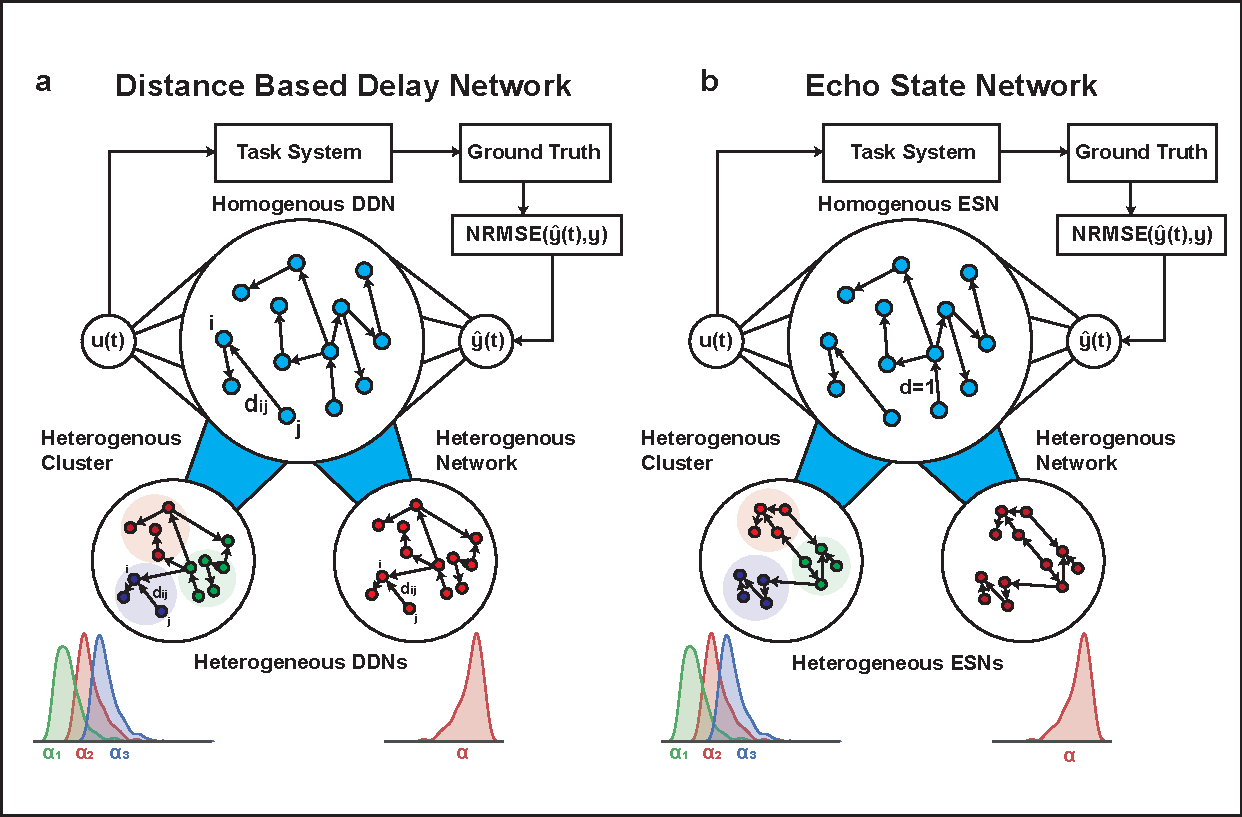
\includegraphics[width=\linewidth]{Figures/Ch_4/network_architecture.pdf}
    \caption{\textbf{Reservoir architecture and heterogeneity design in DDNs and ESNs:} \textbf{(a)} DDNs were made heterogeneous by introducing heterogeniety in delays ($\alpha$), cluster heterogeneity is designed by sampling delays from different distributions for each cluster, similarly, network heterogeneity is designed by sampling delays from a single distribution. \textbf{(b)} same heterogeneity designed for ESNs. It can also be seen that the key difference between ESNs and DDNs are the introduction of delays between units in case of DDNs.   }
    \label{fig:reservoir-arch}
\end{figure}
\subsection{Task Performance }
\subsubsection{NARMA 30}

In order to study the effect of heterogeneity in leak parameters in ESNs and DDNs, we evaluated the networks using their validation scores for each generation of CMA-ES algorithm shown in \textbf{Fig. \ref{fig:eval}a} while these networks learn to perform NARMA-30 task (see Methods). It can be seen that as the networks are optimized over generations, the validation scores lower for both ESNs and DDNs, but the NRMSE scores for DDNs, especially DDNs with network wide fixed decay, per cluster distributed decay and per cluster fixed decay are much lower than ESNs. It can also be seen that all ESNs are optimized to similar NRMSE scores. Interestingly, it can be seen that DDNs with per-cluster fixed decay out perform, DDNs with higher levels of heterogeneity, while the DDNs with network wide distributed decay showed similar performance as the ESNs. We also evaluated the performance of the best optimized networks on a test set shown in \textbf{Fig. \ref{fig:eval}b}, it can be seen that DDNs with network wide fixed decay has lower NRMSE score than ESNs. For per-cluster case, the performance of DDNs and ESNs are indistinguishable. 

\subsubsection{Mackey-Glass}
Similar to the NARMA-30 task we optimized ESNs and DDNs with varying levels of heterogeneity for Mackey-Glass time series prediction task (see Methods section ), we evaluated the performance of the networks using prediction horizon metric (see Methods section ), it can be seen from \textbf{Fig. \ref{fig:eval}b} that prediction horizons for validation run over generation of CMA-ES optimization for DDNs are consistently higher than the ESNs. It can also be seen that DDNs with network wide distributed decay performs the best among all the DDNs, reaching the prediction horizon of 500 steps. It is also noticeable that ESNs with per cluster distributed decay and network wide fixed decay perform the worse compared to all other variants. ESNs with network wide distributed decay and per cluster fixed decay perform objectively better, reaching a prediction horizon value of 300 steps.  Similar to the NARMA-30 taks, we evaluated the performance of the best optimized networks on a test set shown in \textbf{Fig. \ref{fig:eval}b}, it can be seen that DDNs with network wide fixed decay has lower NRMSE score than ESNs.

\begin{figure}
    \centering
    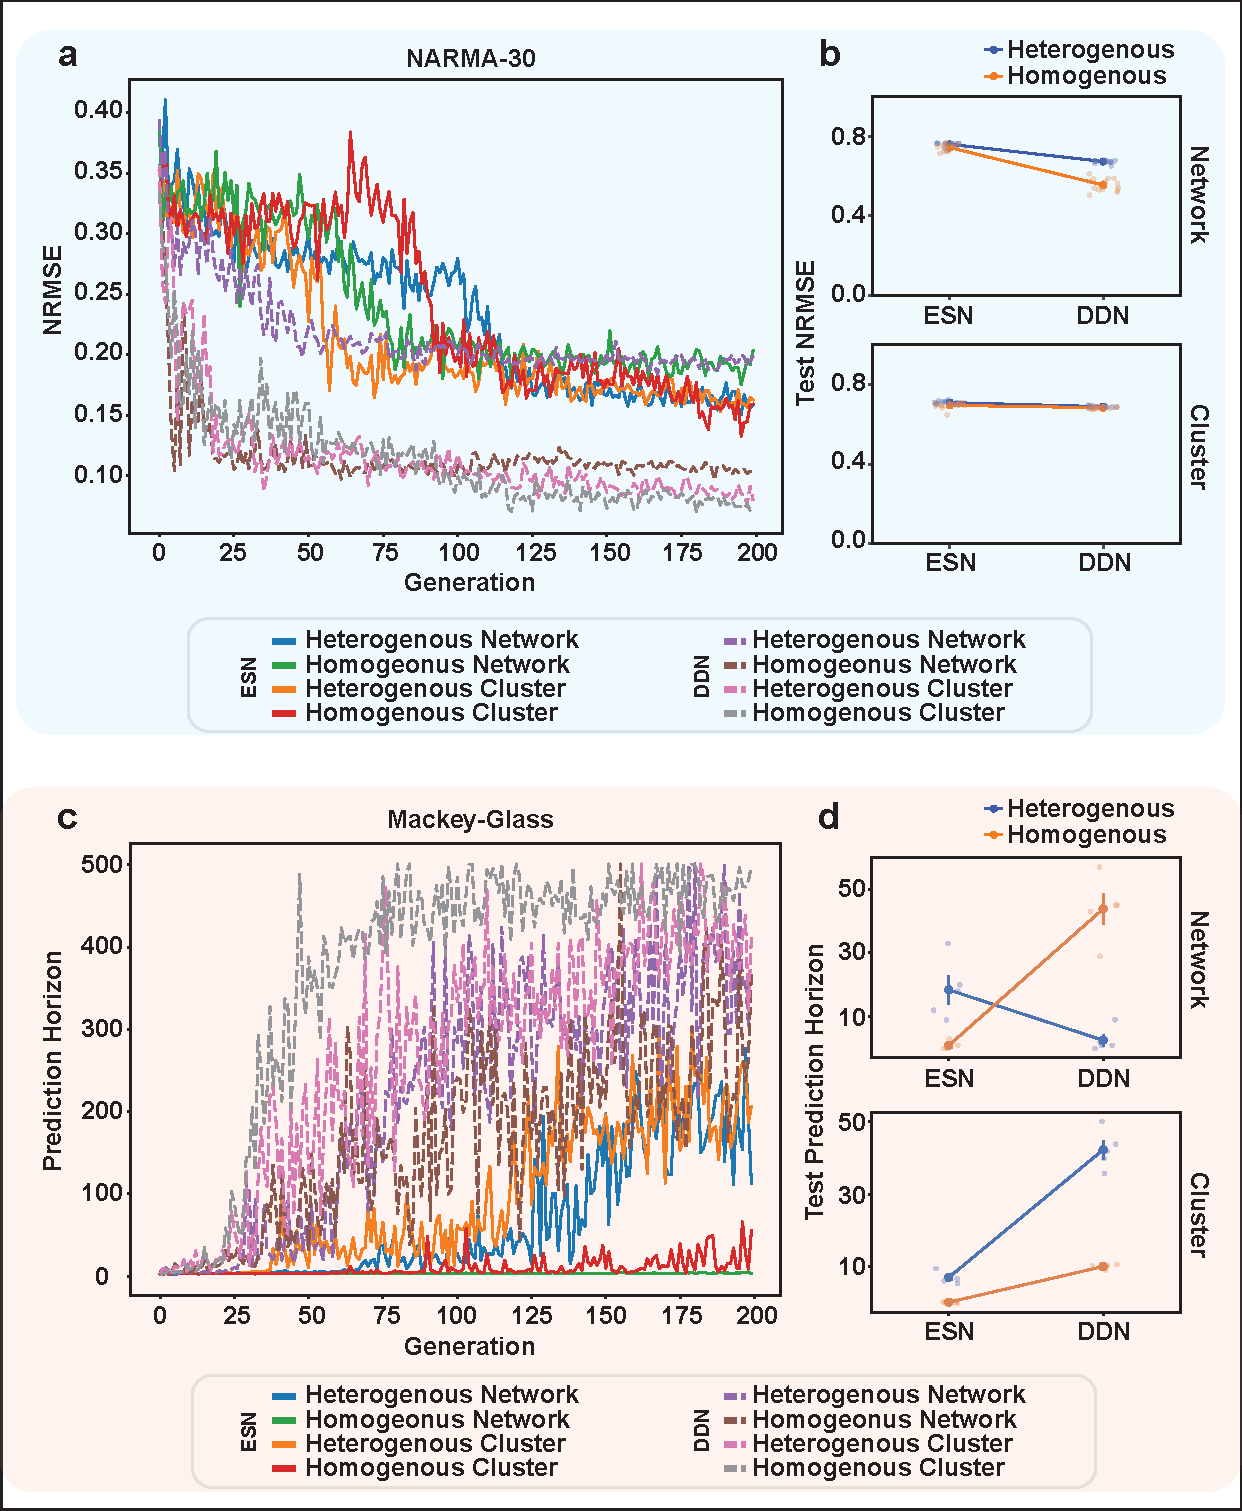
\includegraphics[width=\linewidth]{Figures/Ch_4/Task_performance.pdf}
    \caption{\textbf{Network performance for DDNs and ESNs with or without heterogeneity}: \textbf{(a)} Line plot shows the perforamce in terms of NRMSE over generation during CMA-ES optimization for DDNs and ESNs during NARMA 30 task.  
    }
    \label{fig:eval}
\end{figure}

\begin{figure}

\textbf{(b)} Test NRMSE for different network configurations for both ESNs and DDNs. It can be seen that DDNs with/without heterogeneity perform better than ESNs. \textbf{(c)} Performance of ESNs and DDNs with or without heterogeneity optimized for Mackey-Glass prediction task over generations of CMA-ES optimization. \textbf{(d)} Test performance of ESNs and DDNs optimized for Mackey-Glass timeseries prediction task, separated based on heterogeneity types.
\end{figure}

\subsection{Stability and Dimensionality}
\subsubsection{Maximum Lyapunov exponents}
In order to evaluate the advantage of intrinsic heterogeneity on ESNs and DDNs we calculated the largest lyapunov exponents of the sampled best networks while they perform the task (see Methods section). This was done in order to examine the stability of the network dynamics while the networks perform the task, we hypothesized that intrinsic decay heterogeneity might cause the networks to be more chaotic than their homogeneous counterparts. We evaluated the Maximum Lyapunov exponents for each network and heterogeneity types for different perturbation magnitudes ranging from $1e^{-1}$ to $1e^{-9}$. We perform this analysis for NARMA-30 and Mackey-Glass tasks separately, the results are summarized in \textbf{Fig. \ref{fig:lyapunov}a-b}. 

For NARMA-30 task (\textbf{Fig. \ref{fig:lyapunov}a}), it can be seen that for each perturbation magnitude, the largest lyapunov exponent are negative for all ESNs variants and are lower than DDNs, suggesting that ESNs have more contracting dynamic than DDNs despite the heterogeneity. The outlier to this observation is the ESN with network wide fixed delay, for which the lyapunov exponent is negative but invariant to the perturbation magnitude and comparable to DDNs. It is also important to observe that for all perturbation magnitudes, the highest perturbation yields the lowest exponent. In case of DDNs, the per cluster fixed decay configuration the maximum lyapunov exponent was invariant to the perturbation magnitude. The MLE for DNNs with network wide distributed decay and per cluster distributed decay were comparable, on the other hand, DDNs with network wide fixed decay shows a positive MLE for highest magnitude perturbation ($1e^{-1}$) suggesting chaotic dynamics. 

For Mackey-Glass timeseries prediction task (\textbf{Fig. \ref{fig:lyapunov}b}), it can be seen that for each perturbation magnitude, the largest lyapunov exponent are negative for all ESNs variants and are lower than DDNs, suggesting that ESNs have more contracting dynamic than DDNs for this task as well, despite the heterogeneity. It is also important to observe that for all perturbation magnitudes, the highest perturbation yields the lowest exponent just as in case of NARMA-30. The ESNs with network wide distributed decay were found to have the highest MLE among ESNs and the ESNs with per cluster fixed decay were found to have the lowest MLE. In case of DDNs, the per cluster fixed decay configuration shows a positive exponent for the  magnitude of $1e^-9$ and $1e^-7$. The MLE for DNNs with all other variants had comparable negative MLE for all each perturbation magnitude suggesting a stable contracting dynamic. 

\subsubsection{Dimensionality}
In order to further evaluate the usefulness of intrinsic heterogeneity in terms of recruiting reservoir units for performing the task, we calculated the dimensionality of the network using the network states while the network is driven by the task input. We hypothesized that intrinsic decay heterogeneity might increase the dimensionality of the network, improving the task performance. We drove the network with NARMA-30 and Mackey-Glass input for 2000 steps, and used the network state after 300 steps of warm-up period. For NARMA-30 task, we observed low dimensionality for all networks, the highest for ESN with fixed decay per cluster (D=15) and lowest for DDNs with network wide fixed decay (D=8), distributed decay per cluster (D=8) and fixed decay per cluster (D=8). Similarly, for Mackey-glass time series prediction task, we observe low dimensionality for all networks except for ESNs with distributed decay per cluster (D=98). The network with lowest dimension was found to be DDNs with fixed decay per cluster. Overall, this shows that both ESNs and DDNs do not recruit a high number of units in order to perform both NARMA-30 and Mackey-glass tasks.      

\begin{figure}[!htpb]
    \centering
    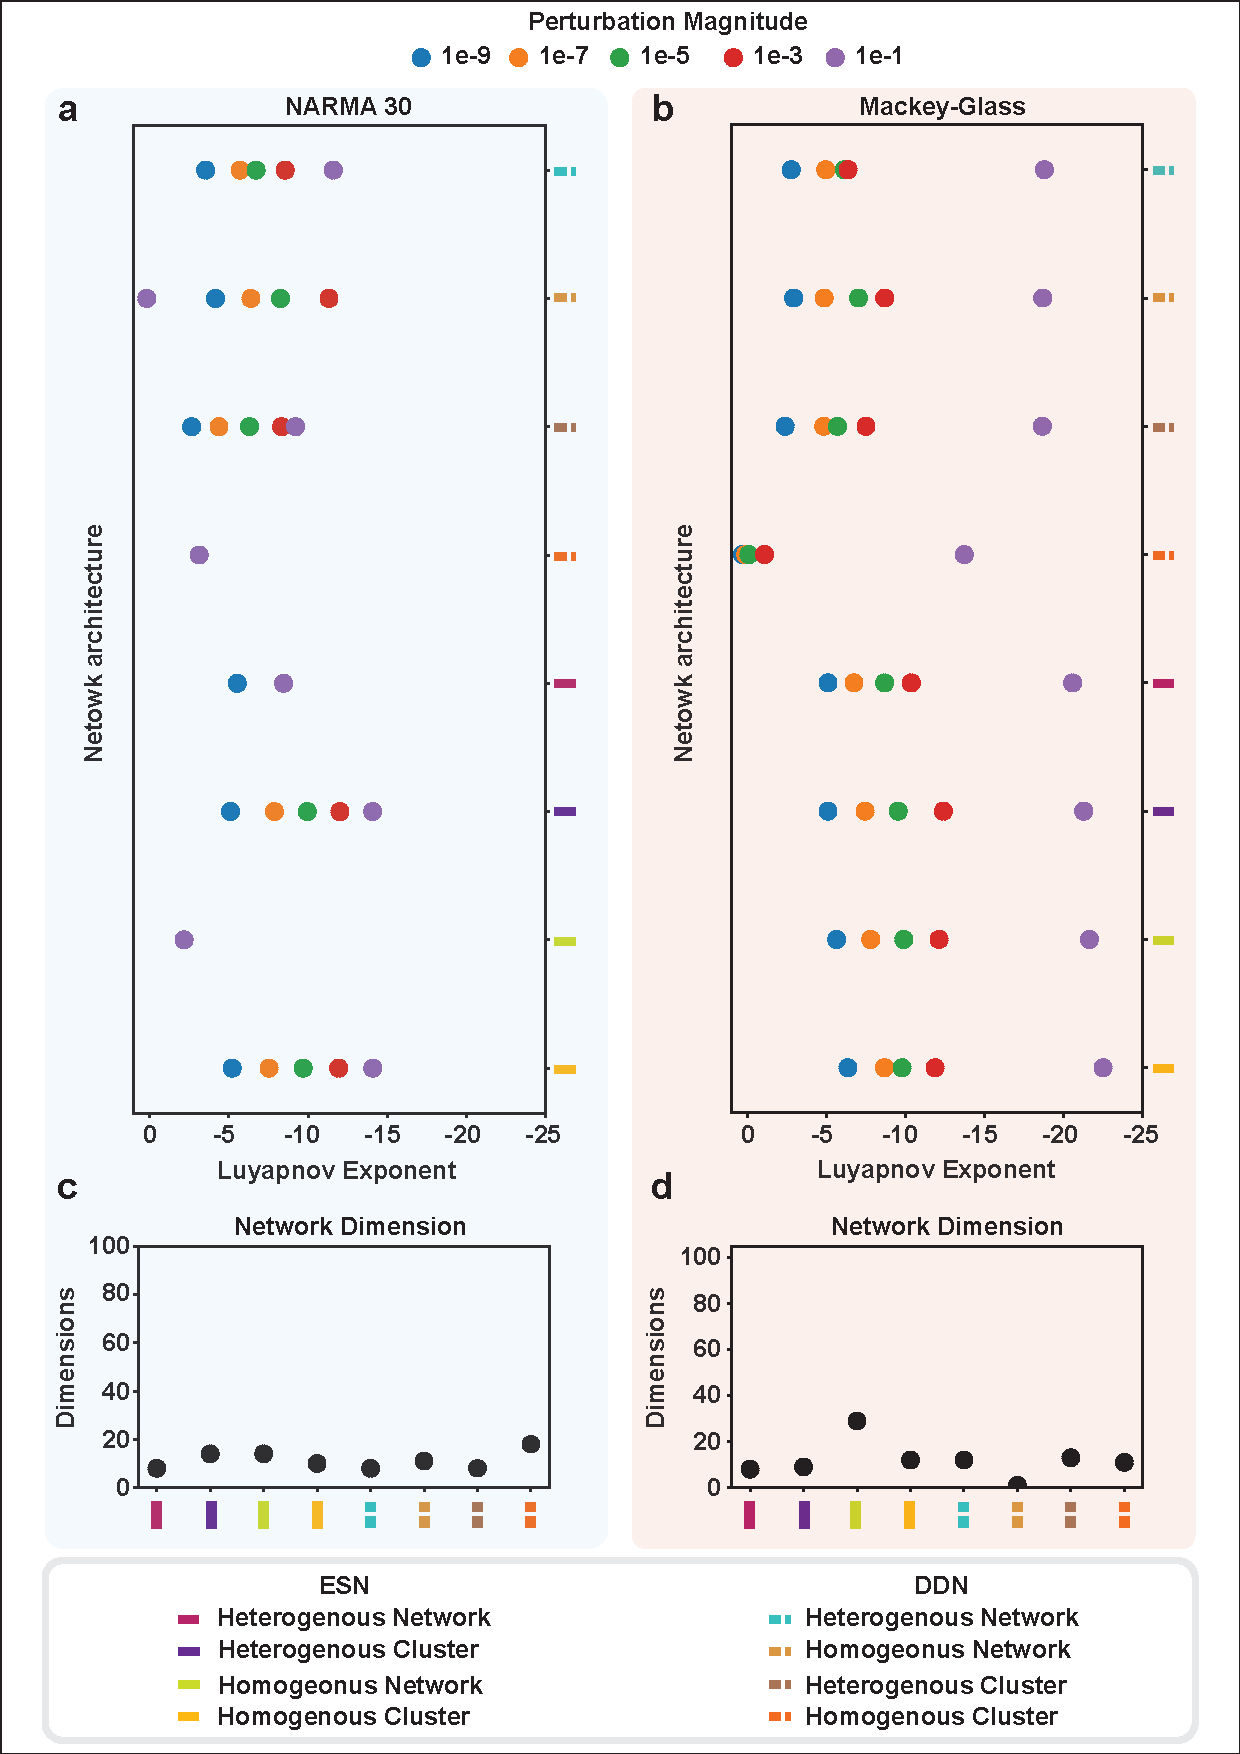
\includegraphics[width=0.8\linewidth]{Figures/Ch_4/Luyapnov_dimensions.pdf}
    \caption{\textbf{Dynamics based on Lyapunov exponent and dimensionality of optimized networks:} \textbf{(a-b)} shows the Lyapunov exponents of the optimized networks while performing the NARMA 30  (blue background) and Mackey-Glass (red background). \textbf{(c-d)} shows the network dimensionality while performing the NARMA 30 (blue background) and Mackey-Glass timeseries prediction tasks (red background).}
    \label{fig:lyapunov}
\end{figure}

\subsection{Linear Memory capacity}

In order to understand if intrinsic decay heterogeneity has an effect on the memory of ESNs and DDNs, especially to see if networks with heterogeneous decay parameters change the way networks store temporal information, especially the number of time steps these networks can recall information from, we calculated the linear memory capacity (see methods section). We used the maximum delay of 40 steps. The observed linear memory capacity for each network variant is summarized on \textbf{Fig. \ref{fig:MC}}. 


For the NARMA-30 task (\textbf{Fig. \ref{fig:MC} left}), it can be seen that every ESN variant has the capacity to recall from upto 20 time steps ago and the capacity is distributed over all the steps between 0 and 20, we do not observe a stark improvement in the memory capacity as a result of heterogeneity.  On the other hand, DDNs show a much more nuanced difference in terms of memory distribution for NARMA-30 task, DDNs with fixed decay per cluster show a concentration of capacity at 3 different time steps, while DDNs with distributed decay per cluster show a prominent concentration at two delay steps. It is also clearly observed that DDNs do not utilize the time window closer to the input, creating a except for DDNs with network wide fixed decay. This suggests that ESNs have limited mobility to recall the past steps in order to perfrom the task, and decay heterogeneity doesn't provide any improvement on this. While, DDNs scatter the capacity more sparsely, thus utilizing the past states more strategically.         

For the Mackey-Glass time series prediction task (\textbf{Fig. \ref{fig:MC} left}), it can be seen that every ESN variant ustilizes just a few past states from when the input is received, most of the capacity is recruited from just the previous step, we do not observe a stark improvement in the memory capacity as a result of heterogeneity for the case of Mackey-Glass as well. On the other hand, DDNs show a much more variability, DDNs with network wide distributed decay and DDNs with distributed decay per cluster, show a wide spread capacity over multiple delay steps, while DDNs with fixed values show a concentration of capacity around 10 time steps ago. 

This goes to show that while for ESNs, the decay heterogeneity doesn't change drastically, for DDNs, the memory capacity is altered due to decay heterogeneity, therefore aiding in task performance. 


\begin{figure}
    \centering
    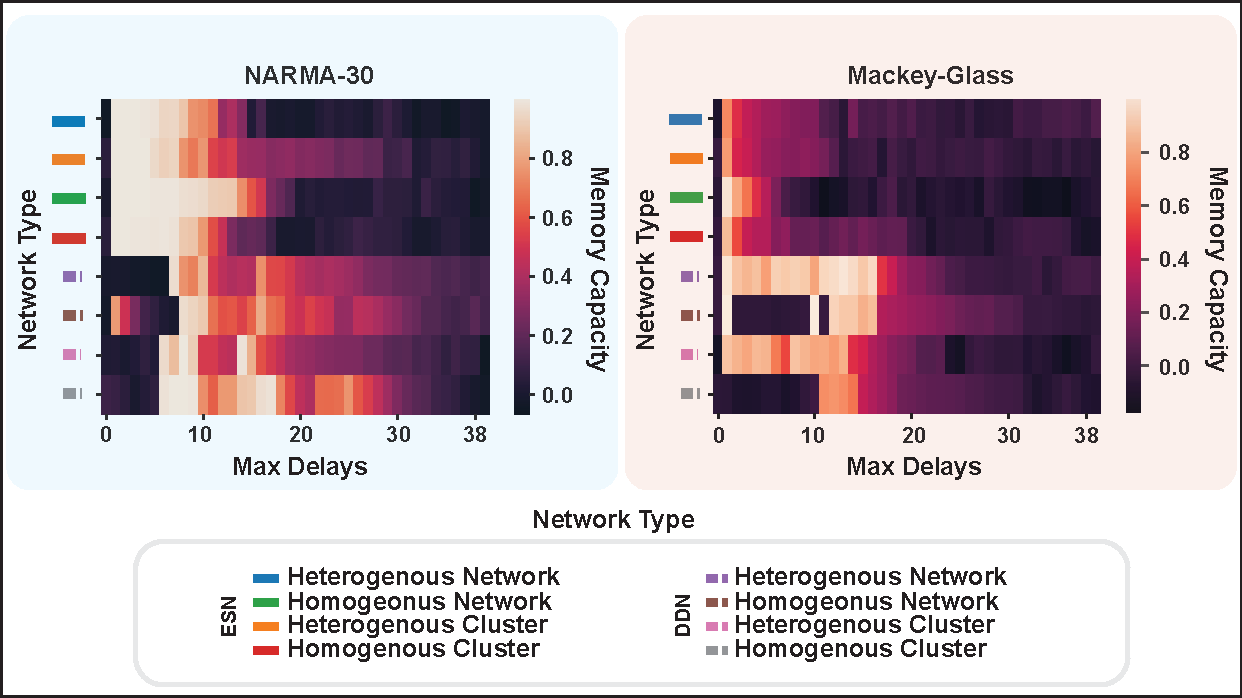
\includegraphics[width=\linewidth]{Figures/Ch_4/LInear MC.pdf}
    \caption{\textbf{Linear Memory Capacity of optimized networks}: \textbf{(Left)} Linear memory capacity of the networks optimized for NARMA 30 task for different delays. \textbf{(Right)} Linear memory capacity of the networks optimized for Mackey-Glass time series prediction task for different delays. }
    \label{fig:MC}
\end{figure}


\newpage

\newpage
\section{Discussion}


This study aimed at studying the effect of timescale (decay parameter) heterogeneity of individual units in reservoir networks on their computational performance, particularly in ESNs and DDNs. Set across two benchmark tasks namely, NARMA-30 and Mackey-Glass, and across four heterogeneity configurations. We found that across all heterogeneity configurations, DDNs outperform ESNs in both tasks. This confirms previous work showing that delay-based architectures are better suited for memory-intensive tasks \cite{iacob2022distance}, this can be because the introduction of time delays enables more flexible temporal dynamics, even more so than inherent decay, rendering inherent decay redundant. We observed that ESNs trained on NARMA-30 task, homogeneous cluster performs the best. But not for the Mackey-Glass task, where ESNs with Heterogeneous cluster, shows the best performance. Surprisingly, homogeneous network DDNs outperform heterogeneous network ESNs, suggesting that architectural delay mechanisms alone offer substantial computational benefits extending the hypothesis \cite{tanaka2022reservoir} that diverse timescales enhance network performance in both DDNs and ESNs.

The ultimate best-performing configuration across both tasks was the homogeneous cluster DDNs. This suggests that structured, modular heterogeneity in decay parameters is more beneficial than randomly distributed heterogeneity. One likely reason is that this setup creates functionally specialized subpopulations with different integration windows, which quite common in biological neural circuits. It allows the reservoir to simultaneously retain short and long term dependencies spread across multiple units. These results support the hypothesis rooted in neuroscience that the diversity of timescales is functionally beneficial for temporal processing and memory \cite{Lundqvist2016gamma, Runyan2017timescales, Cavanagh2020diverse}. 

Contrary to our initial hypothesis, networks with decay heterogeneity did not show increased instability. In fact, all ESNs remained in a contracting regime, with strongly negative Lyapunov exponents across perturbation magnitudes. DDNs were more variable, with some configurations (e.g., Homogeneous network) approaching neutral or even slightly positive exponents under high perturbation. This suggests that DDNs trade off stability for richer dynamics, and that heterogeneity does not necessarily lead to chaotic or unstable behavior. Interestingly, for all network types, the largest perturbation magnitude yielded the most negative Lyapunov exponent. This is likely due to saturation or nonlinear contraction in state space, and highlights the importance of evaluating stability in the local (infinitesimal) regime to interpret true Lyapunov behavior.

We hypothesized that decay heterogeneity would increase the effective dimensionality of the network enabling richer representations. This was not supported. Most networks exhibited relatively low-dimensional dynamics, with little difference between configurations. This could mean that the tasks at hand do not require high-dimensional embeddings, or that the reservoirs learn to compress relevant dynamics efficiently regardless of heterogeneity. It may also suggest that stability and memory, not dimensionality, are the primary contributors to performance in this setting.

Linear memory capacity analysis revealed a more nuanced story. While ESNs showed limited changes across heterogeneity types, DDNs exhibited significant differences in how memory was distributed. Notably, DDNs with distributed decay showed wider memory spread, while fixed-decay variants concentrated memory at specific lags. This suggests that decay heterogeneity allows DDNs to strategically allocate memory a critical property for tasks like NARMA, where both recent and delayed inputs matter. This behavior was absent in ESNs, which tended to have more rigid, shallow memory profiles regardless of heterogeneity.

This study is limited to two benchmark tasks and a specific class of recurrent models. Future work should explore: Broader tasks, including those involving categorical sequence prediction or noisy real-world data, other forms of heterogeneity (e.g., in connectivity, input weights), how decay heterogeneity interacts with delay heterogeneity under more complex learning rules or online adaptation. It would also be valuable to explore the Information processing capacity of these systems, and how dimensionality evolves over time or under different input statistics.

Our results suggest that introducing modular heterogeneity in decay dynamics can meaningfully improve performance and memory organization in reservoir networks particularly when paired with architectural delays. From a neuroscience perspective, this supports the idea that diverse time constants in biological systems are not incidental, but serve computational roles such as memory stratification and temporal coding.

From an engineering viewpoint, these findings argue for designing non-uniform, structured reservoirs in artificial systems, especially for tasks involving long-range dependencies or multi-timescale dynamics. Rather than tuning a single decay or leak parameter, practitioners could benefit from multi-cluster architectures with targeted decay profiles.


\newpage


\begin{spacing}{1.0} % Set the line spacing to single spacing
\fontsize{8pt}{8pt}\selectfont
\bibliographystyle{apalike} %%%%Changed
\renewcommand{\bibname}{References}
\bibliography{All_bibtex} %%%%Changed
\end{spacing} % restore the line spacing to original
% \printbibliography

%-------------------------------------------
\chapter{General Discussion} 
% \ChapFrame 
\thispagestyle{empty}
\AddToShipoutPictureBG*{%
  \AtPageLowerLeft{%
    \begin{tikzpicture}[remember picture, overlay]
      \node[inner sep=0] at (current page.center) {\includegraphics[width=\paperwidth, height=\paperheight]{Figures/6.pdf}};
    \end{tikzpicture}
  }
}

% \begin{tikzpicture}[remember picture, overlay]
%   \node[anchor=north, xshift=0.4cm , yshift=-3.5cm] at (current page.north)  {\includegraphics[scale=0.7]{Figures/cover_line4_glow.png}};
% \end{tikzpicture}
\fancyhf{}
\fancyhead[C]{Chapter 5. General Discussion}% <- added
\fancyfoot[R]{\thepage\ifodd\value{page}\else\hfill\fi}
%\fancyhead[L]{\ifodd\value{page}\relax\else\hfill\fi Ch \thechapter}
%\renewcommand\headrulewidth{0pt}% default ist .4pt
\renewcommand{\plainheadrulewidth}{.4pt}% default is 0pt


\section{Summary}

The broad aim of this thesis was to shed light on neuronal functional heterogeneity based on context and neuromodulation. The thesis addresses three questions: (1) Is neuronal identity context dependent, and which attributes best capture heterogeneity? (2) How does neuromodulation alter neuronal function? (3) How does intrinsic timescale heterogeneity influence network performance and memory? 

\textbf{Chapter 2} takes on the first research question. It challenges the long-standing assumption in systems neuroscience that neuronal functional identity is fixed. Through direct comparison of neuronal responses to different input regimes, I demonstrated that functional identity of neurons is context-dependent, varying with the nature of the input that neurons receive. Moreover, I provide a framework to compare the electrophysiological features commonly used in functional classification such as action potential dynamics and passive biophysical properties by exploiting the high dimensional functional feature space of neurons and comparing the feature sets and by showing that the linear input filter accounts for a greater proportion of variance across neurons. This makes it a more informative and discriminative feature for functional classification.

In \textbf{Chapter 3}, I took on the second research question. I show that neuromodulation alters information transfer in a cell-type and agonist-specific manner. While previous chapter established the role of input in functional classification and laid out a method to study and compare heterogeneity in high dimensional functional space extracted using a FN input, the influence of neuromodulation on this high-dimensional functional space was still not entirely understood. In this chapter I showed that these neuromodulatory changes in functional properties are not uniformly distributed across the neuronal population; instead, neuromodulation induces shifts in multiple functional properties in a coordinated manner, often making subpopulations more similar in their modulation based changes in functional properties. This adds further complexity to functional classification by showing that identity is not only input-dependent but also dynamically reshaped by internal network states.

Finally in \textbf{Chapter 4}, I extend the investigation of functional heterogeneity in neurons to artificial systems which attempts to answer the third research question. In this chapter I examine how intrinsic timescale heterogeneity affects performance in reservoir computing networks. I demonstrate that Echo State Networks (ESNs) and Distance-Dependent Delay Networks (DDNs) exhibit improved task performance and memory capacity when composed of units with heterogeneous time constants. This supports the idea that structured diversity enhances computational capability both in biological and artificial systems.          

By systematically investigating the research questions discussed above, I introduced a framework to study context based neuronal classification using single unit in-vitro patch clamp recordings. I established that neuronal functional identity depends on the input. I further provided a framework to compare neuronal functional heterogeneity based on four high dimensional attribute sets and show that linear input filter is the most informative feature for studying functional heterogeneity in single neurons. Furthermore, I showed that during a specific neuromodulatory receptor activation, single neurons alter their functional space in heterogeneous manner. Neuromodulation changes the information transfer capabilities of single neurons in a cell-type specific manner and most importantly, due to neuromodulation, the high-dimensional functional space is altered in coordination. Multiple-attribute sets are affected together rather than a single property. Synthesizing our findings from the data-driven investigation of single neurons, I studied the affect of intrinsic heterogeneity on artificial systems such as the reservoir computing systems. My investigation revealed that DDNs and ESNs improve their performance directly due to intrinsic timescale heterogeneity in individual units. I also show that heterogeneity benefits the performance of both ESNs and DDNs but in a task dependent manner. In the following sections I will discuss the broader implications of my findings and the future directions for this research. 


\section{Towards dynamic functional identity of single neurons}

\subsection{Input dependence challenges current taxonomies}

Most long standing efforts towards understanding neuronal heterogeneity have been standing on this assumption that neuronal functional identity is static (\cite{fishell2013neuron, huang2019diversity, markram2004interneurons, mukamel2019perspectives, nelson2006problem, petilla2008petilla, sanes2015types, seung2014neuronal, somogyi2005defined, yuste2020community, zeng2022cell, zeng2017neuronal,komendantov_quantitative_2019}). In \textbf{Chapter 2} I challenge this foundational assumption by showing that neuronal functional identity is context dependent. Despite large-scale classification efforts such as by the Allen Brain Institute (\cite{gouwens2019classification, gouwens2020integrated}), the dependence of electrophysiological types (e-types) on the nature of synaptic input remains largely overlooked. Currently, multi-modal classification efforts combine morphological, electrophysiological and transcriptomic markers together to define cell class. In these studies, a static step protocol is used to extract electrophysiological features. Our study challenges these classification results and demonstrates their input-dependence. Here, I provide evidence that neuronal classification is input-dependent, and that functional identity shifts under different stimulus regimes. This insight calls for a critical reassessment of current classification schemes such as by the Allen Institute (\cite{gouwens2019classification, gouwens2020integrated}) in systems neuroscience. These findings advocate for a paradigm shift: functional classification must be grounded in how neurons respond to realistic, time-varying inputs. Achieving this requires a renewed effort in data collection one that prioritizes dynamic stimulation paradigms. While more resource-intensive, this approach offers a deeper and more meaningful classification for modeling brain computation.


\subsection{Functional value of heterogeneity at the population Level}

In the previous section I described the role of dynamical functional identity in deciding functional classification, but this just one single aspect of the results in \textbf{Chapter 2}. The effect of dynamic functional identity of single neurons needs to be understood on broader scale, at the level of neural circuits. In this section, I aim to highlight the circuit level interpretation of functional heterogeneity. 

In\textbf{ Chapter 2}, STA emerged as uniquely informative for capturing population-level heterogeneity among the four attribute sets (AP, PB, AC and STA). This indicates that even within a single cortical region, the somatosensory cortex, neurons differ substantially in their linear input filters. Such diversity implies a level of functional modularity, where neurons are tuned to distinct input features. This specialization may provide a basis for modularity in cortical computation and aids cognitive flexibility (\cite{wu2025neural,hutt2023intrinsic}). Also, work by (\cite{buonomano2009state}) suggest that activity of a neuron in a network is a complex interaction of the network state at any given instant and the incoming stimuli. This view is completely supported by our finding, as such discarding fixed functional identity. It is likely that this heterogeneity would be even more pronounced when comparing neurons across different cortical areas. These findings argue that cortical models must incorporate variability in feature selectivity to accurately reflect population-level dynamics. 

Having established that STA reveals intrinsic functional heterogeneity, we next asked how this heterogeneity and functional classification can be reconfigured by neuromodulatory signals. In \textbf{Chapter 3}, I use the established framework to study neuromodulatory effects, focusing on dopaminergic (D1, D2) and cholinergic (muscarinic M1) receptor activation. Neuromodulation altered both the amount of information transmitted and the classification of neurons across the four attribute sets. I show that activation of specific receptors reshaped the correlation structure among these features, demonstrating that neuromodulation does not act on single properties in isolation but reorganizes the functional feature space of neurons. Notably, these effects were heterogeneous: subpopulations of neurons responded differently to each receptor agonist, indicating that neuromodulators can act as fine-tuned control mechanisms that selectively modulate specific subsets of the circuit \cite{ogawa2023multitasking,salvan2023serotonin,gast2024neural}. This suggests a dual role for neuromodulation both controlling baseline heterogeneity and exploiting it to regulate population-level dynamics in a context-sensitive manner.

There has been an extensive body of literature that discuss population level control via neuromodulation (\cite{Agnati1995,Fuxe2016,Herrington2016,CervantesSandoval2017,Little2013,Zilles2009,marder2014neuromodulation}). Neuromodulators work thorough volume transmission (\cite{Fuxe2016}), through which they control a group of neurons. Our results provide a direct evidence of this. We show a detailed view of the alteration of functional attributes in subgroups of neurons in the somatosensory cortex and the change in coordination between these functional attributes for a population. Together we show that neuronal identity is dynamic, altered by the input that individual neurons receive together with neuromodulation that altogether alters the network state in which a neuron is embedded by changing subgroups in a heterogeneous manner. Collectively, these findings challenge static taxonomies of cell types and argue for circuit models in which neuronal identity emerges dynamically from combined input and neuromodulatory context. 

\subsection{Introduction of Novel Analytical Methods to Study Functional Reorganization and High-Dimensional Correlations}

Addressing the dynamic nature of neuronal functional classification and heterogeneity required the application of analytical tools not traditionally used in electrophysiological studies. To this end, I employed unsupervised machine learning techniques specifically, Louvain clustering combined with UMAP for dimensionality reduction, and Multi-set Correlation and Factor Analysis (MCFA) (\cite{brown2023multiset}) for feature-space variance comparison.

While Louvain+UMAP has been previously applied to waveform clustering (\cite{lee2021non}), its application to electrophysiological feature spaces across distinct input contexts is novel. This method was useful for classifying high-dimensional attribute(s) extracted from the recordings due to its ability to exploit high-dimensional graph structure for clustering instead of a low dimensional projection which usually results in a loss of nuanced information. And also, due to the fact it is an unsupervised method with a robust hyperparameter selection criteria. In this thesis, I leveraged this framework to directly compare neuronal classifications under different stimulation regimes (e.g., step current vs. frozen noise), revealing context-dependent shifts in functional identity.

A persistent challenge in electrophysiological classification is the lack of consensus on which features most effectively capture neuronal heterogeneity. To move beyond arbitrary or limited feature selection, I employed MCFA to quantify the correlation structure across multiple high-dimensional attribute sets. This method allowed us to compare high dimensional attribute sets to identify the shared and private variance structure between the attribute sets. This allowed us to identify which sets are most informative for characterizing functional diversity. Furthermore, we used MCFA to assess how these correlation structures change under neuromodulatory influence, offering new insight into how functional properties reorganize in response to network state changes. 

Although UMAP+Louvain clustering and MCFA are established tools in genomics and single-cell omics (\cite{brown2023multiset}), their adoption in systems neuroscience remains limited. This thesis demonstrates their applicability to electrophysiological data and advocates for their broader use in analyzing the high-dimensional functional landscape of neurons. With more comprehensive datasets, these methods are likely to yield deeper, more robust insights into functional heterogeneity and neuronal classification. We also expect these methods to be adapted more widely for many other problem domains in neuroscience.

\section{Computational modeling implications}

I showed in \textbf{Chapter 2} and \textbf{Chapter 3} using single unit recordings that cortical neurons are heterogeneous in their functional properties and in the way they respond to neuromodulation. In \textbf{Chapter 4}, I tried to synthesize this observation in artificial system. In order to study the advantage it could have on computational properties of reservoir computing systems. 

\subsection{Heterogeneity Improves Reservoir Performance}

In \textbf{Chapter 4}, I demonstrate that timescale heterogeneity enhances the performance of both Echo State Networks (ESNs) and Distance-Dependent Delay Networks (DDNs) on NARMA-30 and Mackey-Glass tasks, particularly in terms of memory capacity and task accuracy. However, we found that the relationship is not monotonous: the most heterogeneous architecture, that is the DNN/ESN with heterogeneous cluster does not always yield the best results. Previous literature has supported structural heterogeneity in artificial networks, where modularity structure improves task performance (\cite{yang2024brain,manneschi2021exploiting}).   

DDNs already incorporate heterogeneous inter-unit delays by design (\cite{iacob2022distance}), which contributes to a more distributed memory profile compared to ESNs (\cite{iacob2022distance}). This structural feature gives DDNs a baseline advantage in tasks requiring temporal integration. Adding intrinsic decay (timescale) heterogeneity further enhances performance as shown in the memory capacity analysis but only up to a point. Beyond a certain level of heterogeneity, the gains diminish or reverse. This result proves the hypothesis by (\cite{tanaka2022reservoir}). This underscores a key insight: the benefits of timescale heterogeneity are task-dependent, and excessive heterogeneity can, in some cases, degrade performance. 

The benchmark tasks reinforce the need to define the optimal timescale heterogeneity, this has also been shown in previous literature to improve performance of spiking networks (\cite{mejias_optimal_2012,zheng2024temporal,tripathy_intermediate_2013,gjorgjieva2016computational,gjorgjieva_intrinsic_2014,duarte_leveraging_2019}). In the NARMA-30 task, which demands precise short-term memory, moderate timescale heterogeneity improved performance in both ESNs and DDNs. In contrast, for the Mackey-Glass task, a chaotic time-series prediction task, excessive heterogeneity introduced instability, reducing predictive accuracy. These results highlight the need to calibrate heterogeneity to the specific computational demands of the task. Various studies on spiking neural networks have demonstrated this task based heterogeneity (\cite{perez-nieves_neural_2021}). Also, intrinsic heterogeneity has been shown to improve encoding performance of spiking networks (\cite{chakraborty_heterogeneous_2022,zeldenrust_efficient_2021,gast2024neural,marsat2010neural}).  

Interestingly, both homogeneous cluster (clusters with singular decay value) and heterogeneous cluster (clusters with decay sampled from a distinct distribution) architectures outperformed fully homogeneous or fully heterogeneous networks across tasks. This suggests that structured heterogeneity variation organized into modular subgroups offers an optimal balance between flexibility (by diversifying time scales for memory) and control (by keeping the network dynamics contracting). This result connects well with the finding in \textbf{Chapter 2-3}, where I show that neuronal population has modularity in terms of modulation and in their intrinsic attributes. These findings emphasize that while intrinsic decay  heterogeneity is beneficial, its impact depends critically on its structure and distribution within the network.



% \subsection{Toward Architecture-Level Design Principles Grounded in Biology}

% \textbf{Chapters 2 and 3} reveal a fundamental insight into the extent and structure of heterogeneity in the somatosensory cortex. By extracting multiple facets of neuronal function including action potential dynamics, adaptation currents, and input selectivity I demonstrate that neurons within a single cortical region vary widely in how they process stimuli. This functional diversity contributes to the brain’s adaptability in responding to dynamic and unpredictable inputs.

% In \textbf{Chapter 4}, I abstracted this biological heterogeneity into artificial systems by implementing it within reservoir computing architectures. The results confirmed a core hypothesis: \textbf{heterogeneity at the unit level enhances the computational performance of interconnected systems}. These findings demonstrate that architectural principles rooted in observed biological phenomena can lead to more effective and flexible artificial systems.

% Moreover, the findings point to a second design insight: heterogeneity must be \textbf{task-aware}. As shown in the benchmark experiments, increasing diversity blindly can be counterproductive. Instead, architectural decisions should reflect both biological principles and task-specific constraints. In this context, “biologically inspired” design must not mean mimicking biology uncritically, but rather \textbf{translating its organizing logic} into systems that serve defined functional goals.

\subsection{Limitations and Methodological Constraints}

In this thesis I have used rigorous analysis and interpretation to show evidence against a static neuronal identity, effect of neuromodulation on neuronal functional space and effect of heterogeneity on the performance of reservoir computing networks. Even though the results are robust, it is important to acknowledge limitations pertaining to the methodology and data. 

First, while frozen noise stimulation provided a richer input space than the step and hold protocols, the overall number of cells recorded under each condition are limited. Consequently, the statistical power for detecting more subtle subpopulation-level effects. This also applies to the recordings for each agonist condition which is a subset of the original data. 

Second, while the classification results revealed clear context- and input-dependent changes in neuronal identity, these findings are currently restricted to neurons within the somatosensory cortex. It remains to be seen whether similar dynamic reconfigurations occur in other cortical or subcortical regions.

Third, the effects of neuromodulation were examined through pharmacological application of D1, D2, and M1 receptor agonists. While this approach isolated the contribution of each receptor type, it does not reflect the full complexity of in vivo neuromodulatory signaling, where multiple pathways act concurrently and interact with behavioral state.

Fourth, the MCFA method is linear in nature, the non-linear interactions between the attribute sets (AP, PB, AC, STA) are not captured by such a method. Therefore, the conclusion about co-regulations especially in case of neuromodulation should be interpreted with caution.  

Finally, in the computational modeling work, the performance of Echo State Networks (ESNs) and Distance-Dependent Delay Networks (DDNs) was benchmarked on a limited set of tasks. The generalizability of the observed heterogeneity and performance relationship to more complex architectures such as deep recurrent models, spiking neural networks, or biologically detailed simulations remains an open question.

While these limitations shape the scope of this study, they do not undermine its central contributions. The results related to heterogeneity remain robust, and the identified limitations instead point to concrete directions for further investigation in the direction of neuronal functional heterogeneity and networks. 

\subsection{Future Directions}

\subsubsection{Biological Extensions}

Future research should aim to extend electrophysiological recordings beyond step current protocols and further embrace dynamic, naturalistic stimulation regimes. One such recording protocol is Dynamic Clamp (\cite{robinson1993injection,sharp1993dynamic}). These would better approximate the range of inputs neurons experience in vivo and provide a richer substrate for functional classification. Additionally, integrating electrophysiology with other modalities such as transcriptomic profiling, morphological reconstruction, or in vivo imaging could yield a more comprehensive, multi-modal map of neuronal heterogeneity.

Another important direction is to link the observed functional reconfigurations induced by neuromodulation to behavior. There has been extensive body of work in this direction (\cite{Ott2023,Picciotto2012,Walters1987,Nadim2014,robinson2004firing}), which link the neuromodulation of single neurons by dopamine and acetylcholine to reward and learning. But comprehensive high-dimensional view of single neurons' functional space is missing. This potential area of research could involve combining neuromodulatory manipulation with behavioral paradigms and recording from populations in active animals, allowing us to trace how shifts in input filters or feature selectivity translate into changes in perception or motor output.

An important missing link in the context of our finding is the mechanistic explanation of heterogeneity found in linear input filters of the somatosensory neurons, a mechanistic understanding of how relatively homogeneous PB and AP properties give rise to heterogeneous input filters is required. Also, it is an interesting direction to study the effect of input filter heterogeneity in networks. There has been a large body of work such as by (\cite{marder_multiple_2011,marder2014neuromodulation,kumari2024ion, edelman_degeneracy_2001,hennig_constraints_2018}) identifying degeneracy in ion-channel activation and high-level functional properties such as the linear input filter and in a similar way, degeneracy in the activity of single neurons to produce network states. I suggest this direction to get a mechanistic understanding of homogeneity in AP and PB parameters giving rise to heterogeneous linear input filters. 

In Chapter 3 we found the emergence of subpopulations with heterogeneous modulation, it is interesting to pursue this idea on a circuit level to understand how such heterogeneous modulation dives rise to attention in case of dopamine and relate it to behavior in general. This would require a large scale data collection and modeling effort. 

In this thesis I have identified several potential research directions to pursue, which will enhance neuronal taxonomy and neuronal heterogeneity in general, understanding of neuromodulation on circuit level and lead towards mechanistic understanding of varying levels of heterogeneity among the four attribute sets.  

\subsubsection{Computational Extensions}

Besides the future research directions in neurobiology, there are many research direction to be pursued based on the computational part of this thesis. These research directions are aimed at synthesizing knowledge about neuronal heterogeneity and neuromodualtion and use it towards designing biologically inspire neural networks.         

On the modeling side, it will be important to investigate whether the benefits of structured heterogeneity extend to more powerful or biologically plausible architectures, such as spiking neural networks, long short-term memory (LSTM) networks, or transformer-based recurrent systems. A related question is whether heterogeneity should be hand-crafted, as done here, or learned through training a comparison that could provide insight into how diversity emerges through development or adaptation. 

Our network size in the current experiment is small compared to a cortical circuits, a larger network would yield a clearer understanding of the effect of intrinsic heterogeneity on networks. Especially their stability and memory. 

Evolutionary optimization or meta-learning approaches could be used to explore the space of possible heterogeneity structures. These tools may reveal principles for organizing diversity in artificial networks that generalize across tasks, paralleling the diversity we observe in biological circuits.

Finally, for our aim to understand biological underpinnings of heterogeneity in neuronal computation it is important to concern ourselves with biologically realistic networks such as spiking neural networks or cortical networks. Applying the observed heterogeneity in linear input filters and modularity in sub-populations on a network scale such as shown by \cite{liu2021cell} would provide much richer understanding of how these rather orthogonal facets of heterogeneity come together to affect computation.    


\section{Final Conclusion}

In this thesis I show that biologically realistic input is important for neuronal functional classification, moreover, neurons are distinguished by their linear input filter. Taking this idea further, I show that neuromodulators act as a secondary controller of neuronal function, altering information transfer by causing multi-dimensional change in neuronal functional space, I also find sub-population of neurons with distinct modulation profiles. This motivates for a network level study that leverages this sub-population heterogeneity to understand what effect it has on the overall computational properties of neurons. I found that reservoir computing networks benefit from subpopulation level heterogeneity. This showcases the importance of heterogeneity of individual unit. 

\subsection{Epilogue}

It is clear to me that neuronal diversity is not noise, rather a fundamental feature of the brain's architecture. This heterogeneity shapes the structure and function of neural circuits, giving rise to the complexity of behavior, and experience. Therefore, understanding neural diversity is essential not just for neuroscience, but for comprehending the variability that defines human societies. A deeper grasp of this functional diversity is not optional; it is necessary for understanding ourselves and the systems we build.


\newpage
\begin{spacing}{1.0} % Set the line spacing to single spacing
\fontsize{8pt}{8pt}\selectfont
\bibliographystyle{apalike}
\renewcommand{\bibname}{References}
\bibliography{All_bibtex}
\end{spacing}
%-------------------------------------------
\chapter{Supplementary Materials} 
% \ChapFrame
\thispagestyle{empty}
\AddToShipoutPictureBG*{%
  \AtPageLowerLeft{%
    \begin{tikzpicture}[remember picture, overlay]
      \node[inner sep=0] at (current page.center) {\includegraphics[width=\paperwidth, height=\paperheight]{Figures/cover_bg.pdf}};
    \end{tikzpicture}
  }
}

\fancyhf{}
\fancyhead[c]{Chapter 6. Supplementary Materials}% <- added
\fancyfoot[R]{\thepage\ifodd\value{page}\else\hfill\fi}
%\fancyhead[L]{\ifodd\value{page}\relax\else\hfill\fi Ch \thechapter}
%\renewcommand\headrulewidth{0pt}% default ist .4pt
\renewcommand{\plainheadrulewidth}{.4pt}% default is 0pt


\section{Supplementary materials for Chapter 2}

\clearpage
\newpage

\section{Waveform and Action Potential properties manifold \\ comparison }
\begin{figure}[!htpb]
    \centering
    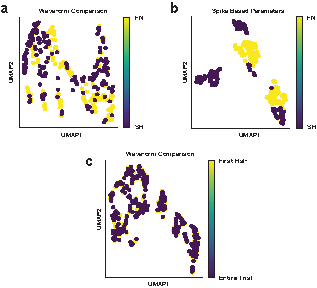
\includegraphics[width=0.8\linewidth]{Figures/Ch_2/appendix1.pdf}
    \caption{(\textbf{a}) Overlaid UMAP representation FN and SH waveforms from 186 neuron used in classification. The waveform shapes are different between SH and FN protocols.(\textbf{b}) FN and SH Action potential parameters used for classification projected together on the same space. The Action potential properties are different between FN and SH protocols. The SH Action potential properties show a bigger spread than FN properties. (\textbf{c}) UMAP projection of averaged Waveform comparison between the first half and the entire trial. The average waveform shape doesn't change as a result of trial length.  }
    \label{first:app1}
\end{figure}
\clearpage

\newpage


\section{Louvain vs Ensemble Clustering for Graphs (ECG) algorithm comparison }
\begin{figure}[!htpb]
    \centering
    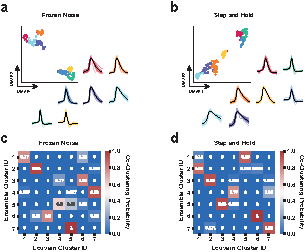
\includegraphics[width=\linewidth]{Figures/Ch_2/appendix2.pdf}
    \caption{(\textbf{a}) UMAP embedding of FN waveforms colored with cluster labels found using Ensemble clustering, with original waveforms in the same color as the respective color. 7 clusters were observed, the same number as in the case of the Louvain community method. (\textbf{b}) UMAP embedding of SH waveforms colored with cluster labels found using Ensemble clustering, with original waveforms in the same color as the respective color. 7 clusters were observed, the same number as in the case of the Louvain community method. (\textbf{c}) Heatmap showing the correspondence between Louvain and Ensemble clustering for graph on FN waveforms. Clusters using the Louvain community detection algorithm show a high correspondence with the clusters obtained using Ensemble clustering for the graph method. (\textbf{d}) Heatmap showing the correspondence between Louvain and Ensemble clustering for graph on SH waveforms. Clusters using the Louvain community detection algorithm show a high correspondence with the clusters obtained using Ensemble clustering for the graph method.}
    \label{first:app2}
\end{figure}
% \begin{figure}
%  \end{figure}
% \clearpage
\newpage

% \label{first:app3}
\section{Cluster stability after leaving one attribute out at a time}
\begin{figure}[!htpb]
    \centering
    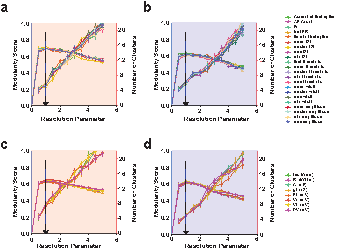
\includegraphics[width=\linewidth]{Figures/Ch_2/appendix3.pdf}
    \caption{(\textbf{a-b}) Stability of clusters for action potential attributes leaving one attribute out for excitatory and Inhibitory sets. The clustering was performed 25 times with random 80\% samples for resolution attributes ranging from 0.0 to 1, the mean and standard deviation of the resulting number of clusters and modularity score are plotted. For the chosen resolution parameter (1.0), the cluster numbers fluctuate between 5-7. The cluster number fluctuates more for the excitatory set (left) than the Inhibitory set (right) (\textbf{c-d}) Stability of clusters for biophysical attributes leaving one attribute out for excitatory and Inhibitory sets. The clustering was performed 25 times with random 90\% samples for resolution parameters ranging from 0.0 to 1, the mean and standard deviation of the resulting number of clusters and modularity score are plotted. For the chosen resolution parameter (1.0), the excitatory population fluctuates between 6-8. On the contrary, the Inhibitory population doesn't show any fluctuation.}
    \label{first:app3}
\end{figure}
\clearpage

\newpage

% \label{first:app4}

\section{Diversity of firing rate and AP half-width}
\begin{figure}[!htpb]
    \centering
    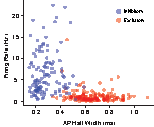
\includegraphics[width=\linewidth]{Figures/Ch_2/appendix4.pdf}
    \caption{Firing rate vs AP half-width between excitatory (red) and inhibitory (blue) populations. The excitatory population has a lower firing rate and higher AP width. The Inhibitory population has a lower AP width and higher firing rate.}
    \label{first:app4}
\end{figure}


\newpage
% \label{first:app5}
\section{STA Heterogeneity}
\begin{figure}[!htpb]
    \centering
    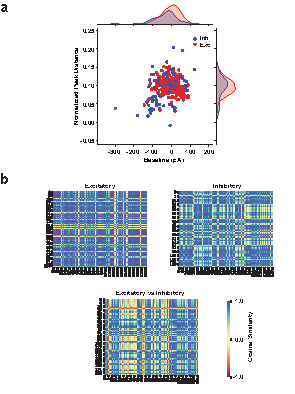
\includegraphics[width=0.8\linewidth]{Figures/Ch_2/appendix5.pdf}
    \caption{{(\textbf{a}) The scatter plot shows the baseline added to the theoretical input vs the Peak distance of the STA. The excitatory population has a higher baseline and higher peak distance. The variance for both baseline and peak distance seems higher for the excitatory population than inhibitory population. (\textbf{b}) The STA cosine similarity is for the excitatory population (top left), the STA cosine similarity is for the inhibitory population (top right), and the STA cosine similarity is between the excitatory and inhibitory populations. The excitatory population has higher similarity than the inhibitory population.}}
    \label{first:app5}
\end{figure}


\clearpage
\newpage
% \label{first:app6}

\section{Cluster assignment likelihood across attributes}
\begin{figure}[!htpb]
    \centering
    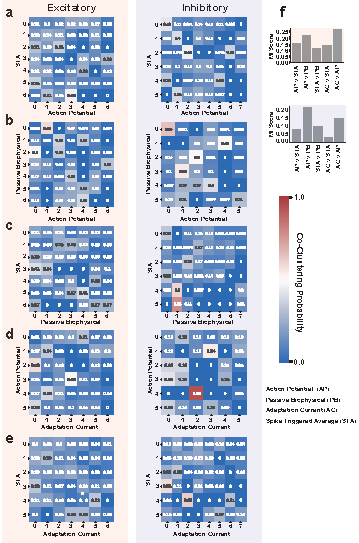
\includegraphics[width=0.8\linewidth]{Figures/Ch_2/appendix6.pdf}
    \caption{(\textbf{a-e}) Heatmap showing the likelihood for neuron clustering in attribute 1 clustering }
    \label{first:app6}
\end{figure}
\begin{figure}
 in one of the clusters in attribute 2 for excitatory (left) and inhibitory (right) population. For each attribute (Action potential, Passive biophysical, STA, Adaptation current ($\eta$), none of the clusters show a high likelihood to be clustering in another attribute. (f) Cluster label comparison between modularity pairs using Mutual information score for excitatory and inhibitory population. None of the pairs reach the modularity of 0.25 showing that neurons cluster differently across attribute sets.
\end{figure}
\clearpage
\newpage

\section{Supplementary materials for Chapter 3}

\newpage


\begin{figure}
    \centering
    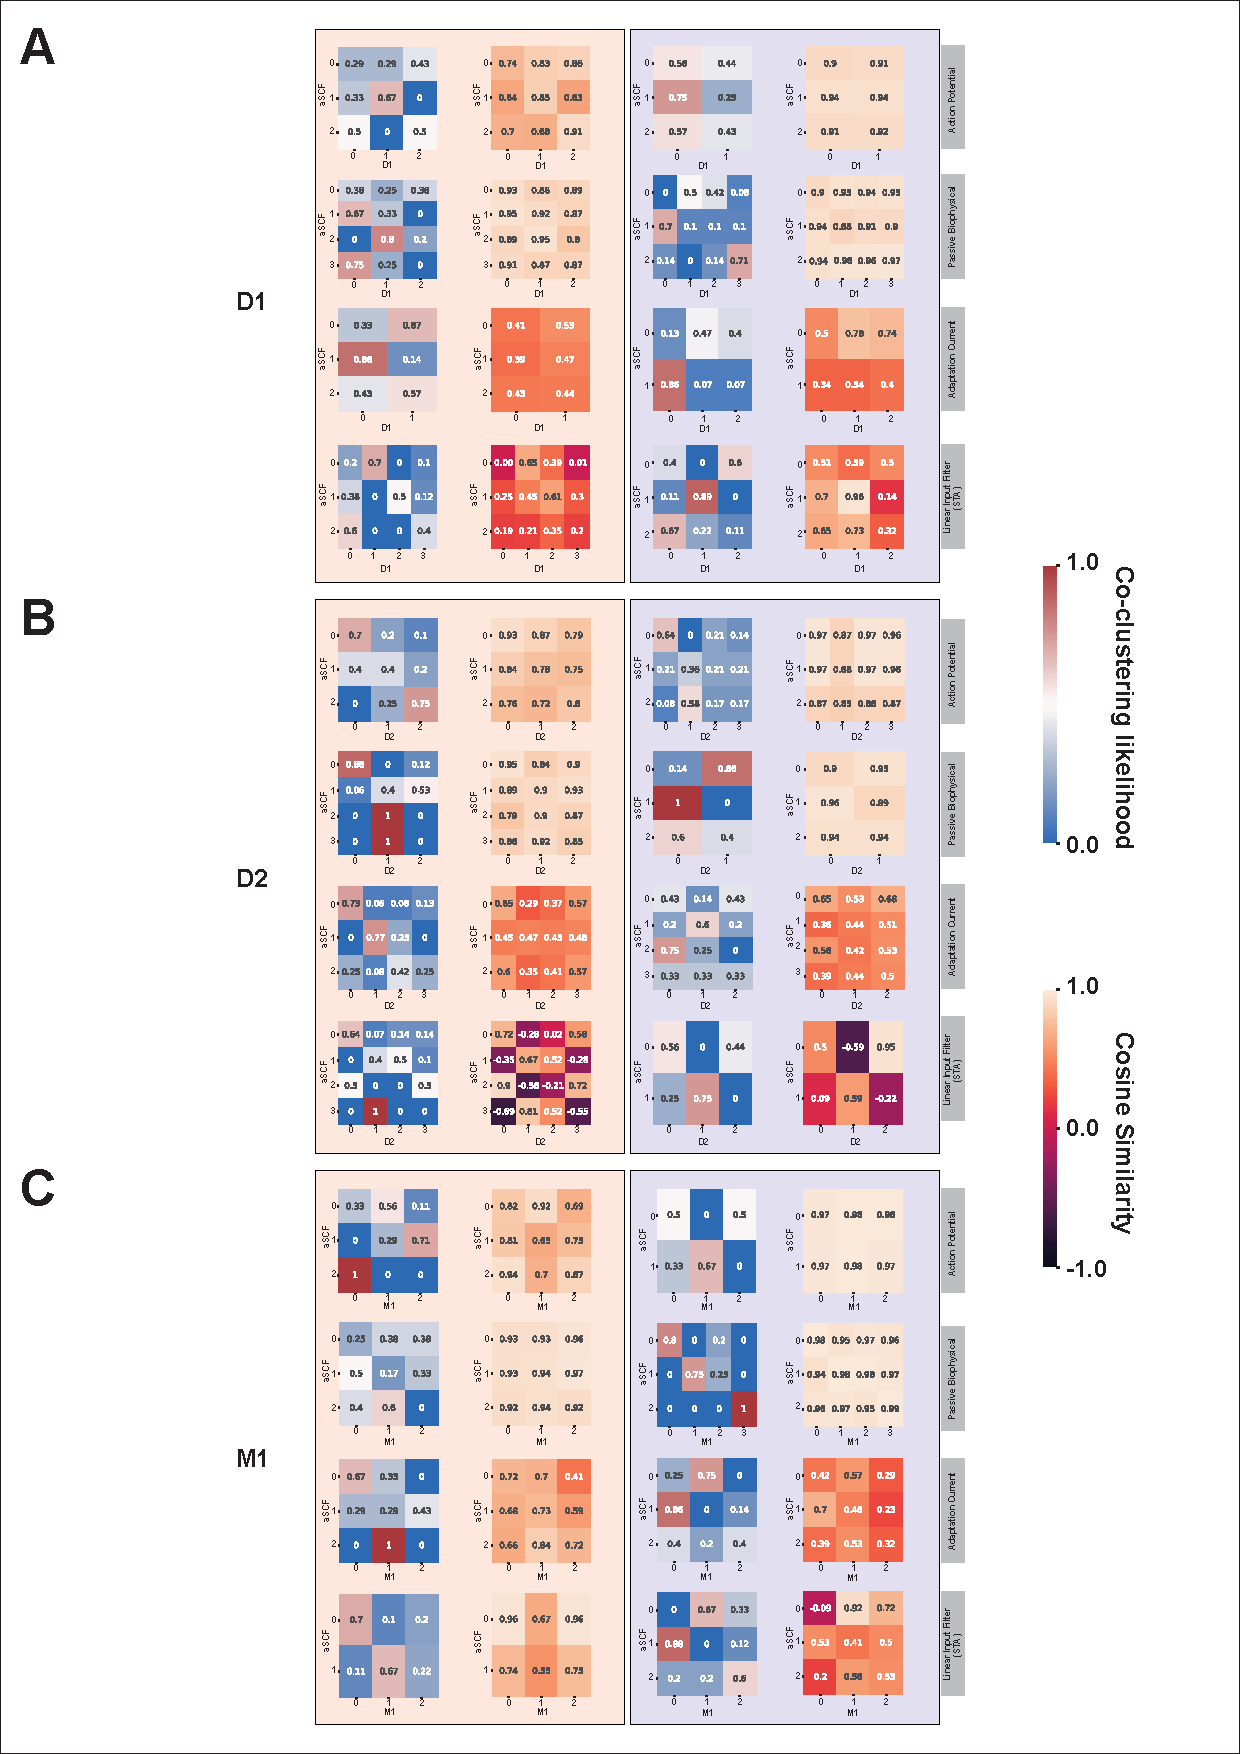
\includegraphics[width=\linewidth]{Figures/Ch_3/Appendix1.pdf}
    \caption{\textbf{Clustering likelihood matrix and cosine similarity across labels shifts for all four properties as a result of neuromodulation for D1-R, D2-R and M1-R}}
    \label{fig:S1_ref}
\end{figure}
\newpage

\begin{figure}
   Top panel shows the cluster likelihood and cosine similarity for D1 vs aCSF trials. Middle shows the cluster likelihood and cosine similarity for D2 vs aCSF trials. Bottom shows the cluster likelihood and cosine similarity for M1 vs aCSF trials.
\end{figure}
\clearpage

\newpage
\begin{figure}
    \centering
    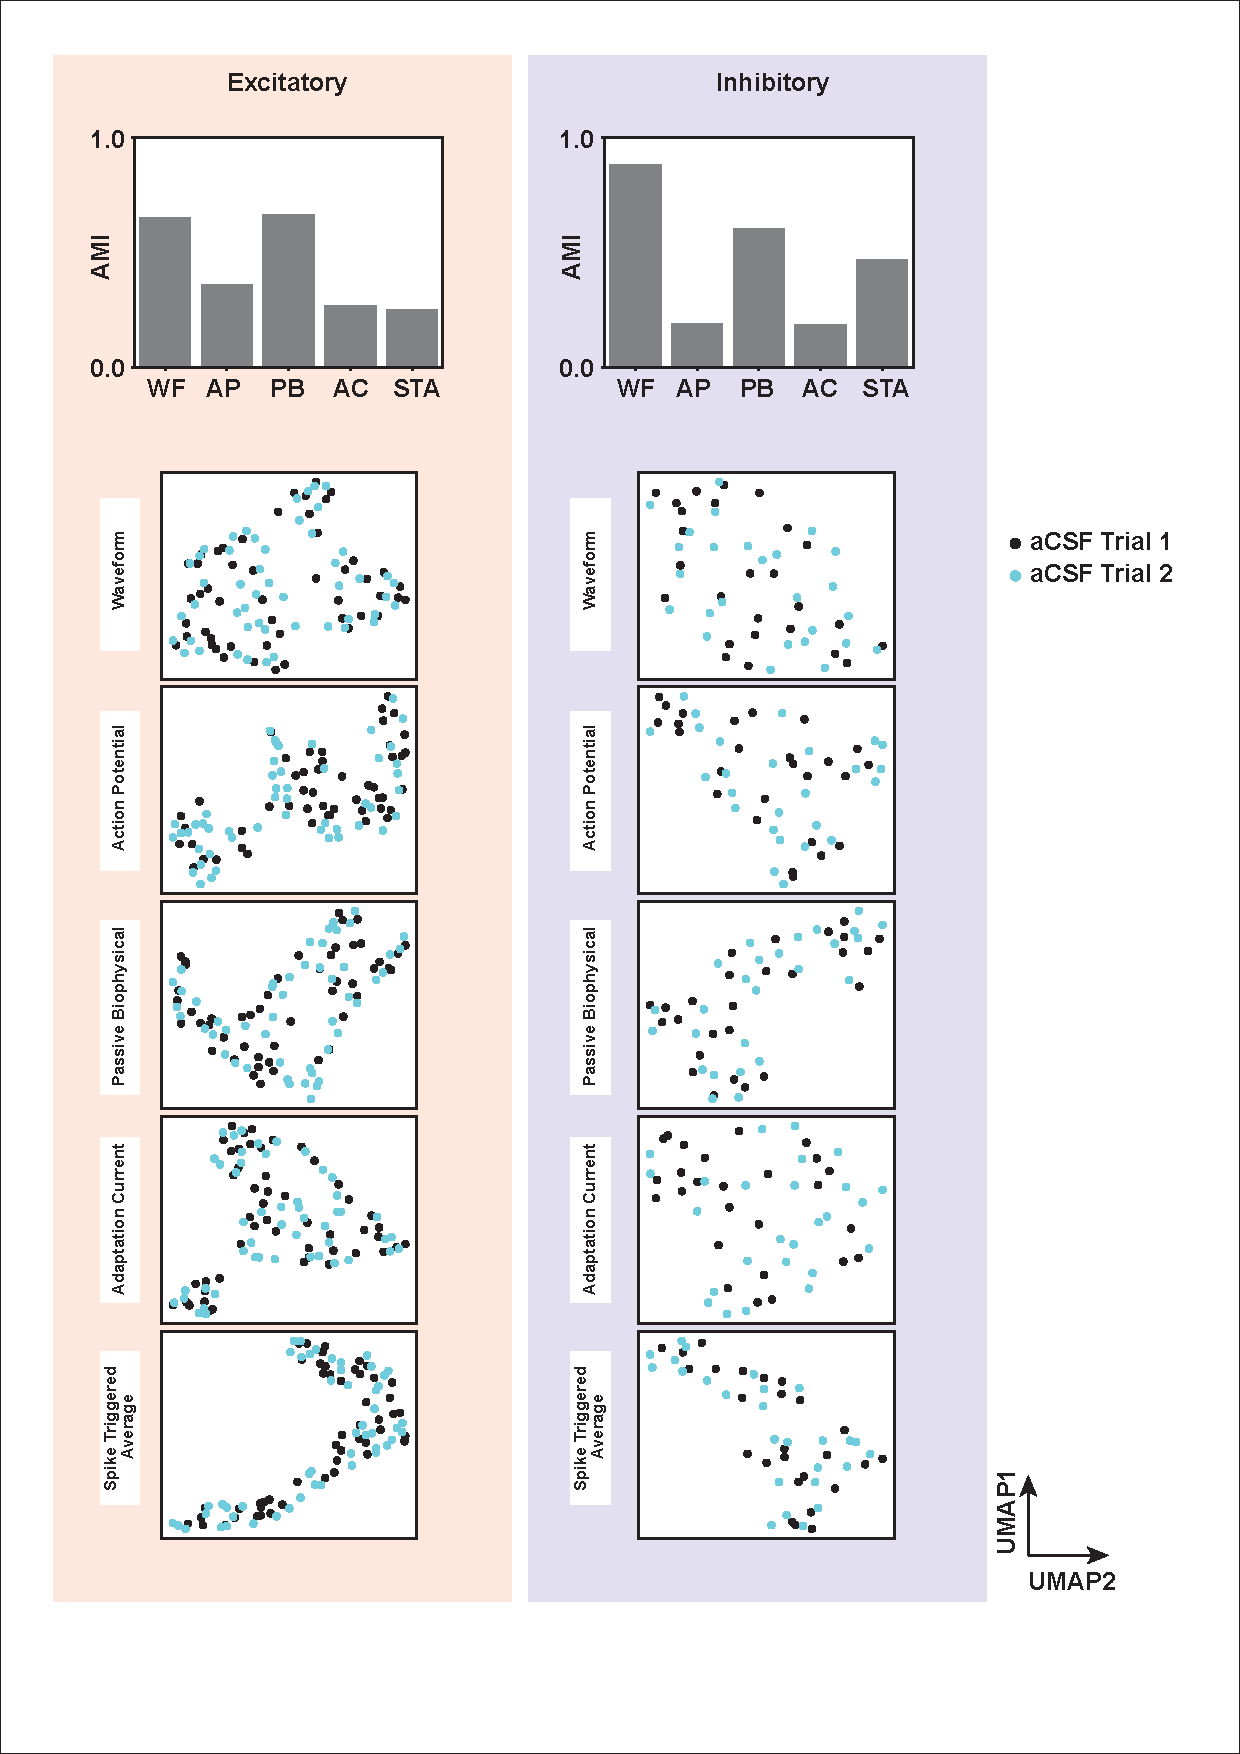
\includegraphics[width=\linewidth]{Figures/Ch_3/Appendix2.pdf}        
    \caption{\textbf{Comparison of aCSF trial 1 vs trial 2 clustering and manifold}}
    \label{fig:S2}
\end{figure}

\begin{figure}
Left and right histograms on top the AMI score between cluster IDs found for aCSF trial 1 vs aCSF trial 2. Waveforms and passive biophysical properties were found to be consistent across the two trials as these properties are not strongly dependent input dynamics. The UMAP plots show the alignment for aCSF trial 1 vs aCSF trial 2.
\end{figure}
\clearpage


\newpage
\begin{figure}
    \centering
    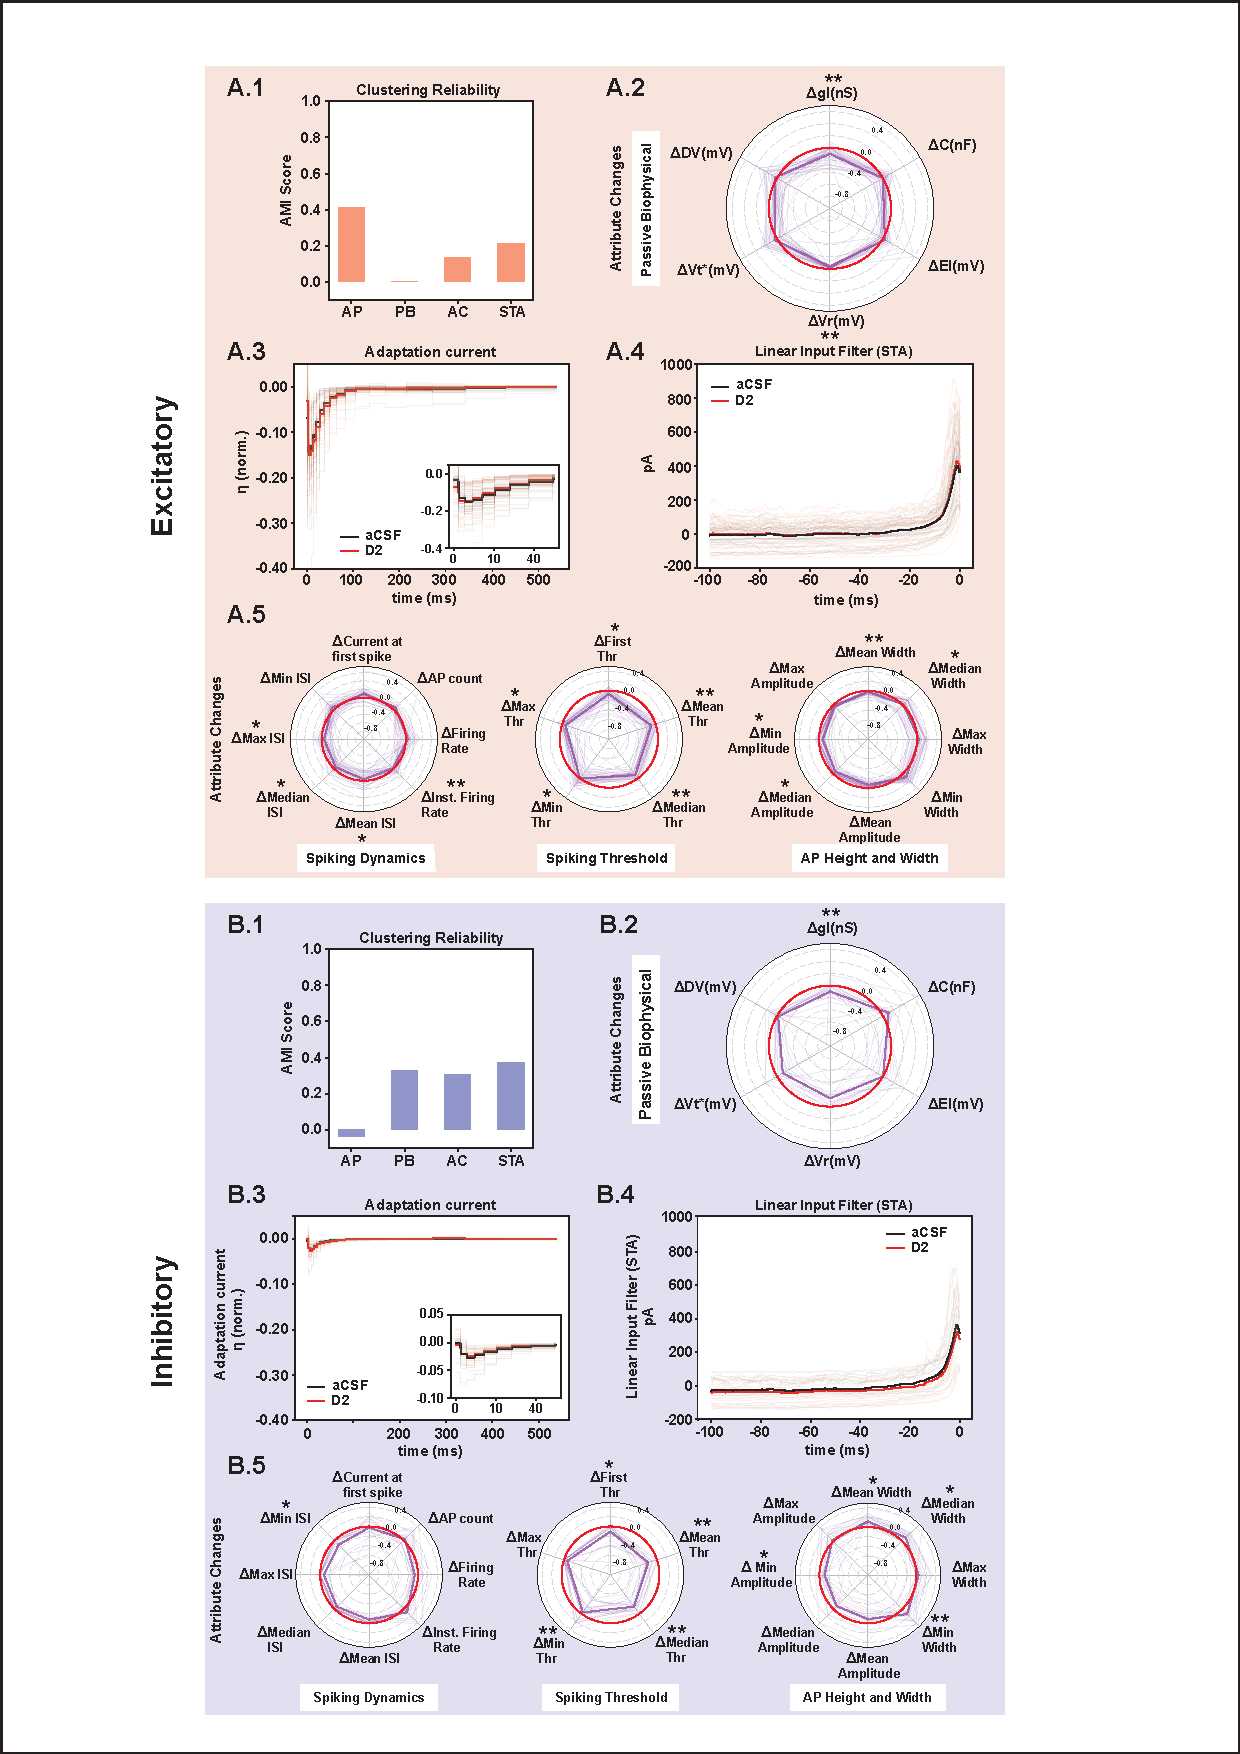
\includegraphics[width=\linewidth]{Figures/Ch_3/Appendix3.pdf}
    \caption{\textbf{D2 receptor activation changes functional clustering and attributes for both excitatory and inhibitory neurons.} }
    \label{fig:S3_ref}
\end{figure}
\newpage
    
\begin{figure}
(\textbf{A.1}) Histogram shows the adjusted mutual information score between the clustering labels obtained for aCSF and D2 trials, the histogram shows a shift in cluster identities as a result of D2 receptor activation across four attributes. (\textbf{A.2}) shows the change in passive parameters with respect to control as a result of D2 receptor activation, normalized by the control trial values. With the mean marked represented with a thick line. (\textbf{A.3}) shows the adaptation current for control (black) and D2 (red), the mean is represented with darker curves. The adaptation current profiles between D2 and aCSF trials were found to be similar. The rise time as well the peak adaptation current between aCSF and D2 were found to be non-significant (see Appendix  \ref{fig:S5}). (\textbf{A.4}) shows the spike triggered average profile for aCSF (black) and D2 (red) trials, the mean is represented with a thick line. (\textbf{A.5}) shows the change in action potential attribute sets with respect to control as a result of D2 receptor activation, normalized by the control trial values. With the mean marked represented with a thick line and the zero line is colored in red. The significant features are marked. \textbf{B.1-5} Same analysis repeated for inhibitory neurons. * $p<0.05$, ** $p<0.001$, *** $p<0.0001$.

\end{figure}
\clearpage

\newpage
\begin{figure}
    \centering
    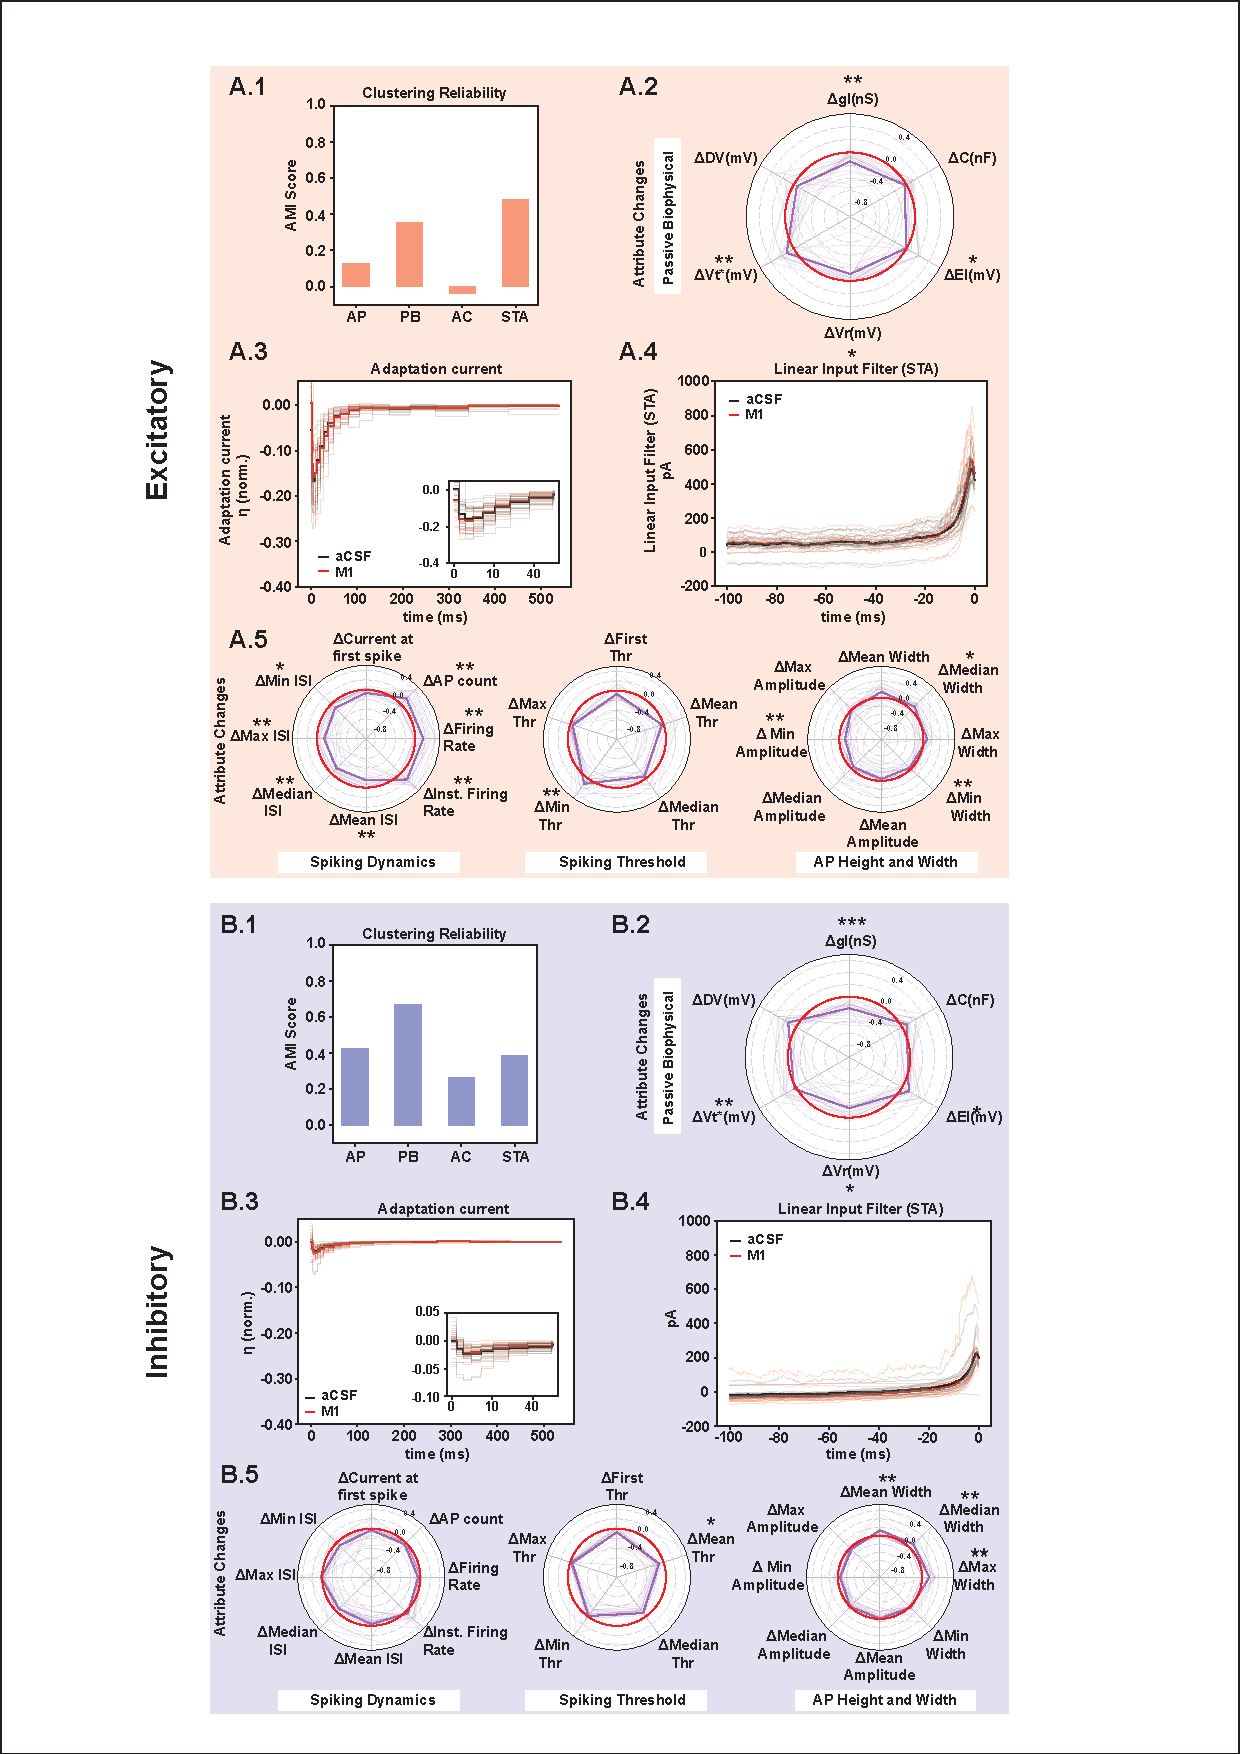
\includegraphics[width=\linewidth]{Figures/Ch_3/Appendix4.pdf}
    \caption{\textbf{M1 receptor activation changes functional clustering and attributes for both excitatory and inhibitory neurons.}}
    \label{fig:S4_ref}
\end{figure}
\newpage

\begin{figure}
(\textbf{A.1}) Histogram shows the adjusted mutual information score between the clustering labels obtained for aCSF and M1 trials, the histogram shows a shift in cluster identities as a result of M1 receptor activation across four attributes. (\textbf{A.2}) shows the change in passive parameters with respect to control as a result of M1 receptor activation, normalized by the control trial values. With the mean marked represented with a thick line. (\textbf{A.3}) shows the adaptation current for control (black) and M1 (red), the mean is represented with darker curves. The adaptation current profiles between M1 and aCSF trials were found to be similar. (\textbf{A.4}) shows the spike triggered average profile for aCSF (black) and M1 (red) trials, the mean is represented with a thick line. (\textbf{A.5}) shows the change in action potential attribute sets with respect to control as a result of M1 receptor activation, normalized by the control trial values. With the mean marked represented with a thick line and the zero line is colored in red. \textbf{B.1-5} Same analysis repeated for inhibitory neurons. * $p<0.05$, ** $p<0.001$, *** $p<0.0001$.

\end{figure}
\clearpage




\newpage
\begin{figure}
    \centering
    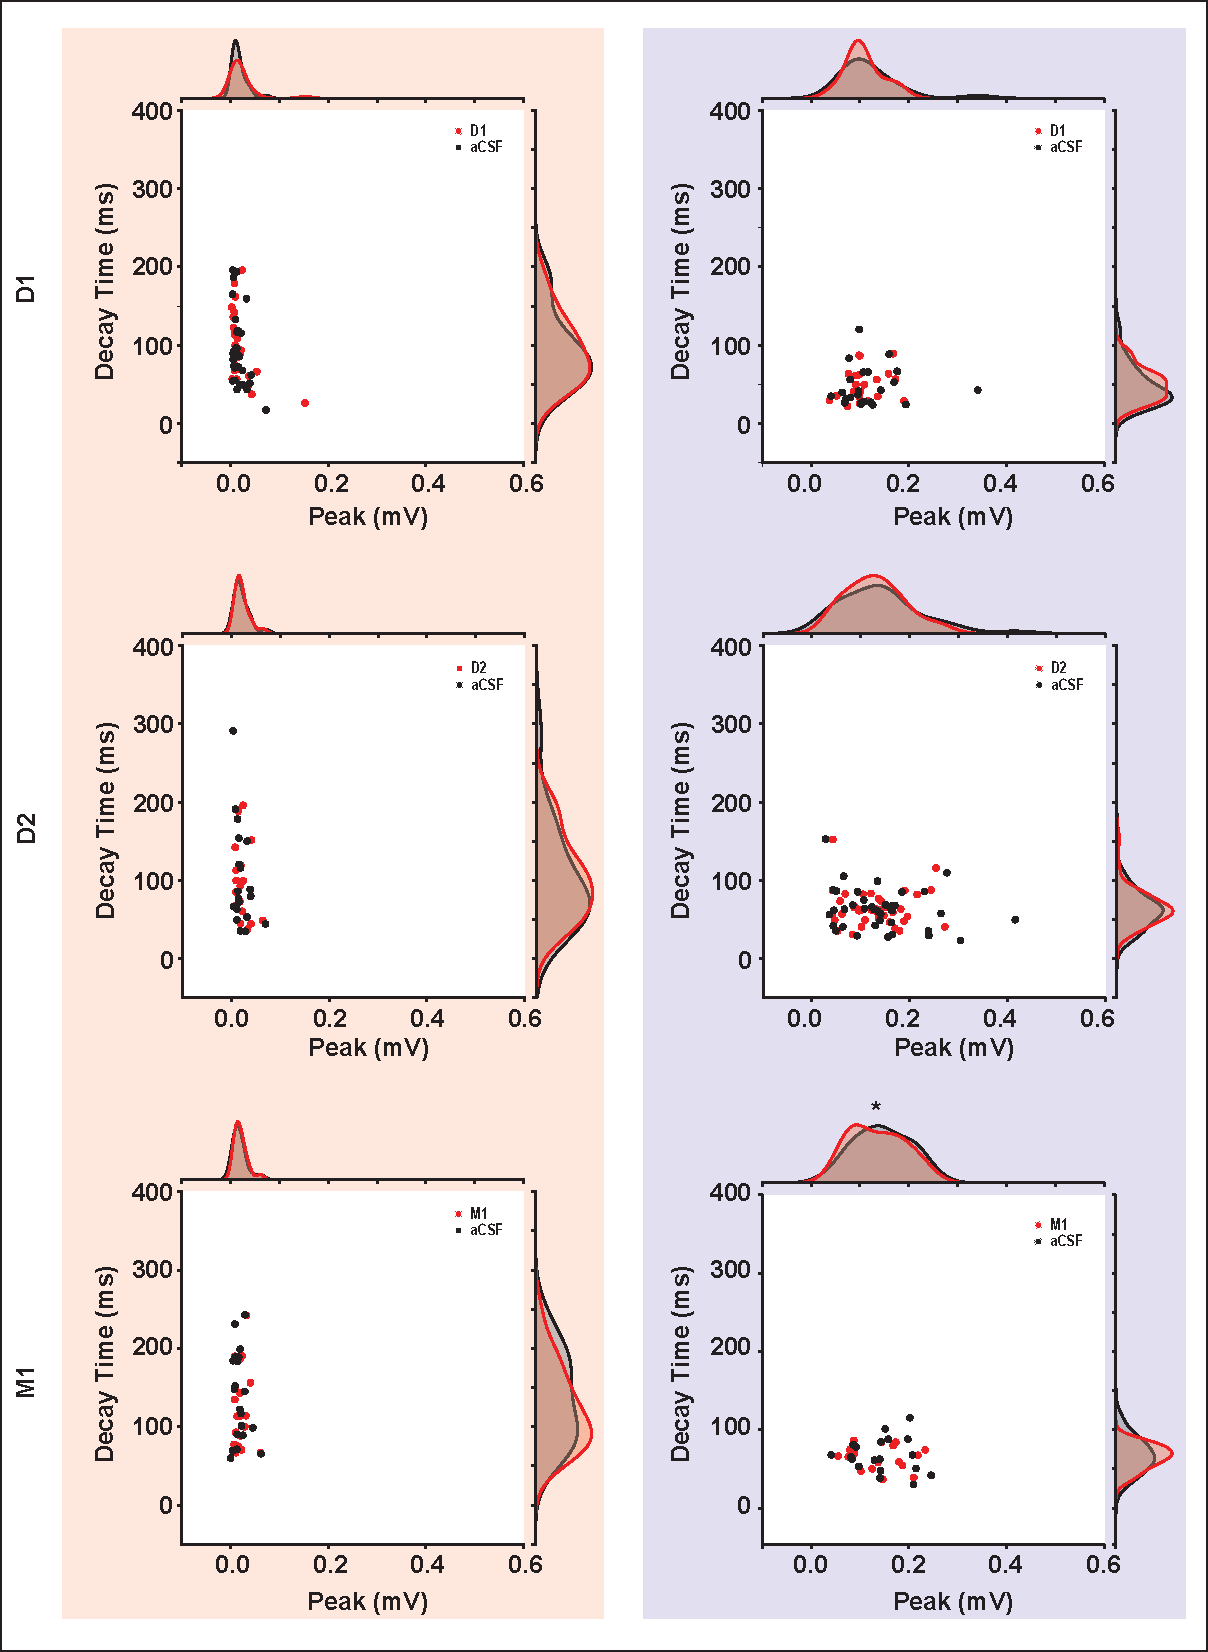
\includegraphics[width=0.9\linewidth]{Figures/Ch_3/Appendix5.pdf}
    \caption{\textbf{Adaptation current peaks and decay times are not strongly altered by D1, D2 and M1 modulation} The scatter plots show the normalized peaks of the AC curve on the x-axis and the decay time for D1, D2 and M1 vs aCSF trials. The red panel represents excitatory and blue panel represents inhibitory.  * $p<0.05$, ** $p<0.001$, *** $p<0.0001$.}
    \label{fig:S5}
\end{figure}

\newpage

\begin{figure}
    \centering
    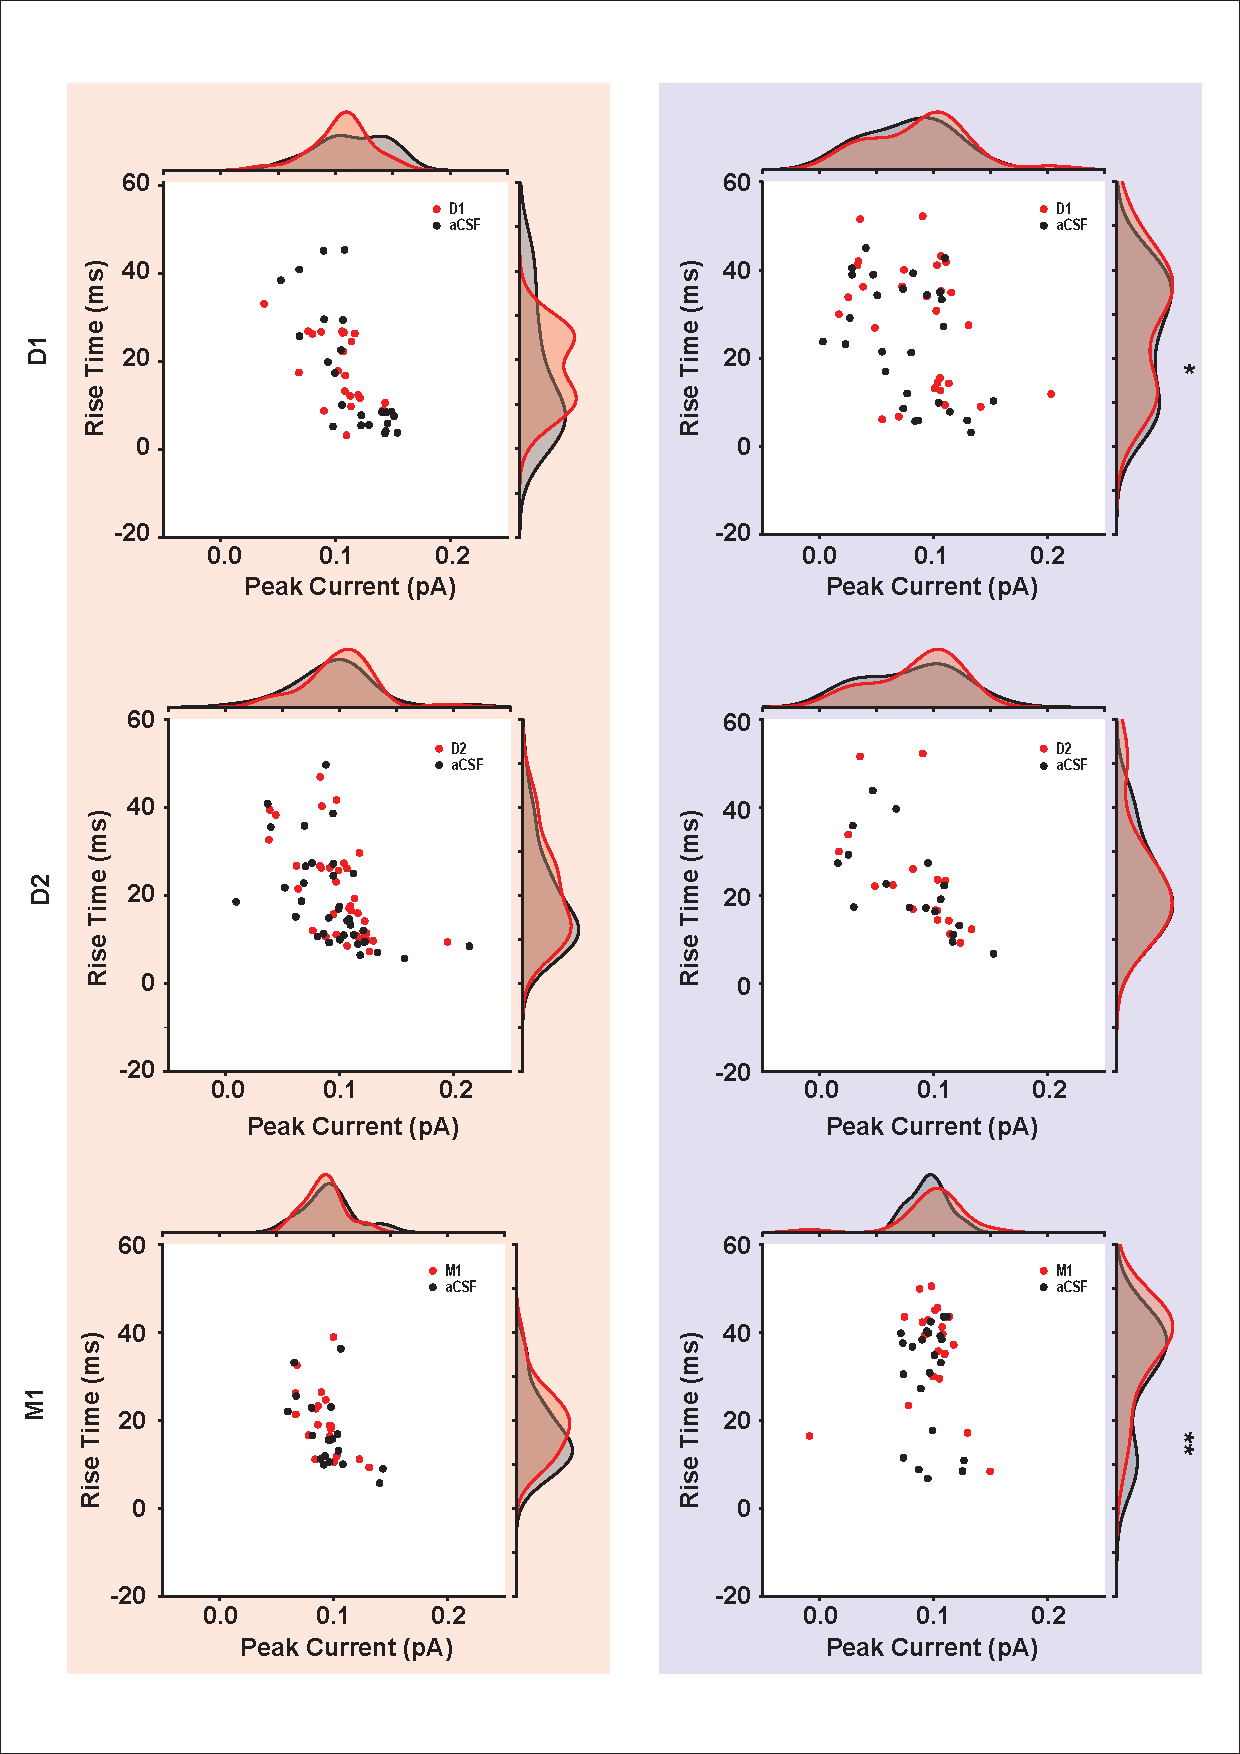
\includegraphics[width=0.9\linewidth]{Figures/Ch_3/Appendix6.pdf}
    \caption{\textbf{Spike triggered average peaks and decay times are modestly altered by D1, D2 and M1 modulation} The scatter plots show the normalized peaks of the STA curve on the x-axis and the decay time for D1, D2 and M1 vs aCSF trials. The red panel represents excitatory and blue panel represents inhibitory population.  * $p<0.05$, ** $p<0.001$, *** $p<0.0001$}
    \label{fig:S6}
\end{figure}
\newpage

\begin{figure}
    \centering
    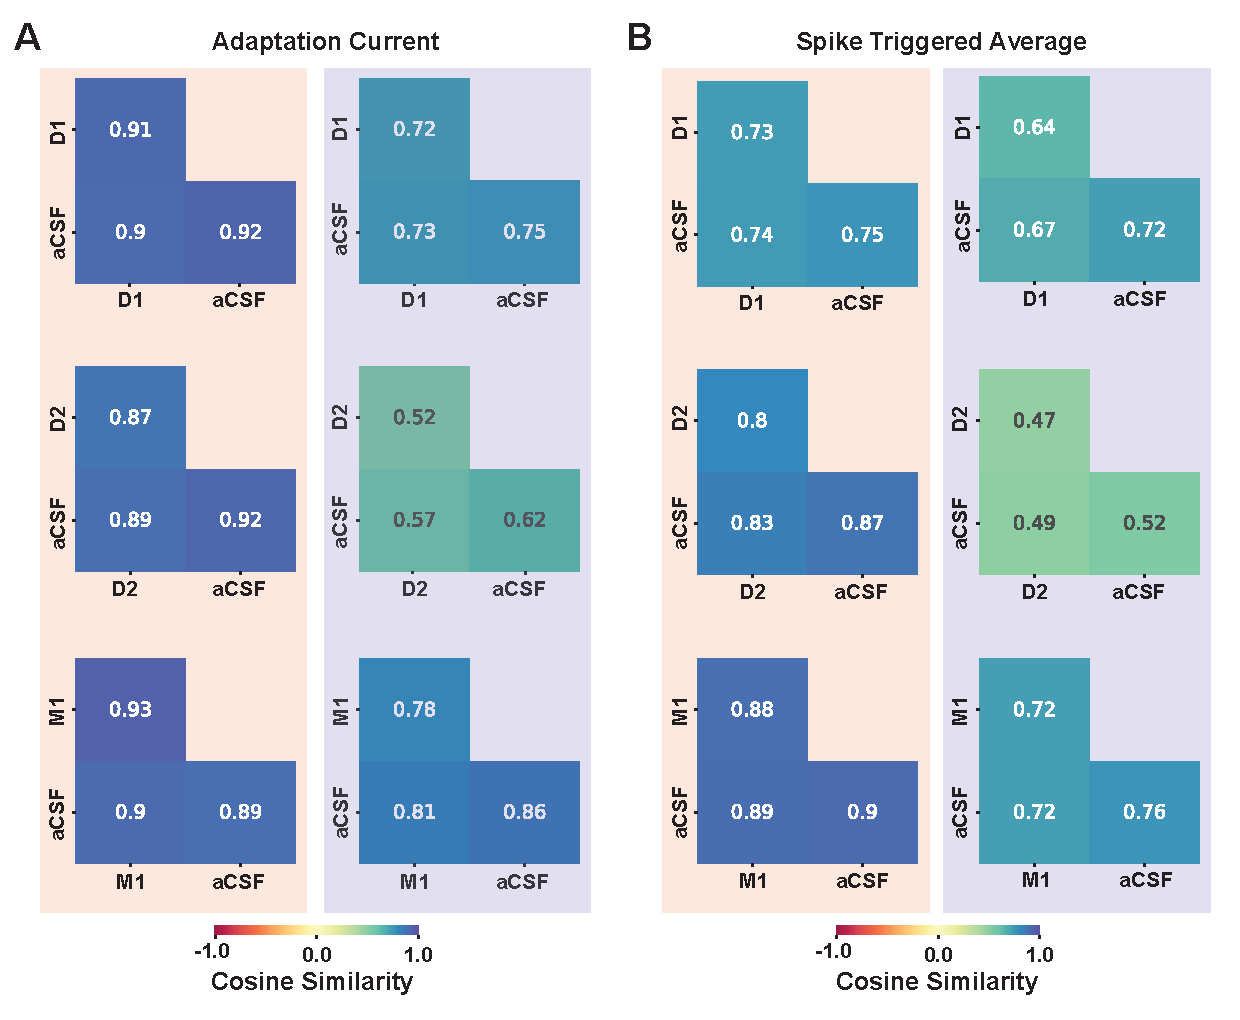
\includegraphics[width=\linewidth]{Figures/Ch_3/Appendix7.pdf}
    \caption{\textbf{Average cosine similarity across and within aCSF-Agonist trials vary in a cell-type specific manner.} (\textbf{A}) Heatmaps show the average AC similarity for excitatory (red background) and inhibitory (blue background) for D1, D2 and M1 vs aCSF trials. (\textbf{B}) Heatmaps show the average STA similarities for excitatory (red background) and inhibitory (blue background) for D1, D2 and M1 vs aCSF trials.}
    \label{fig:S7}
\end{figure}

\newpage

\begin{figure}
    \centering
    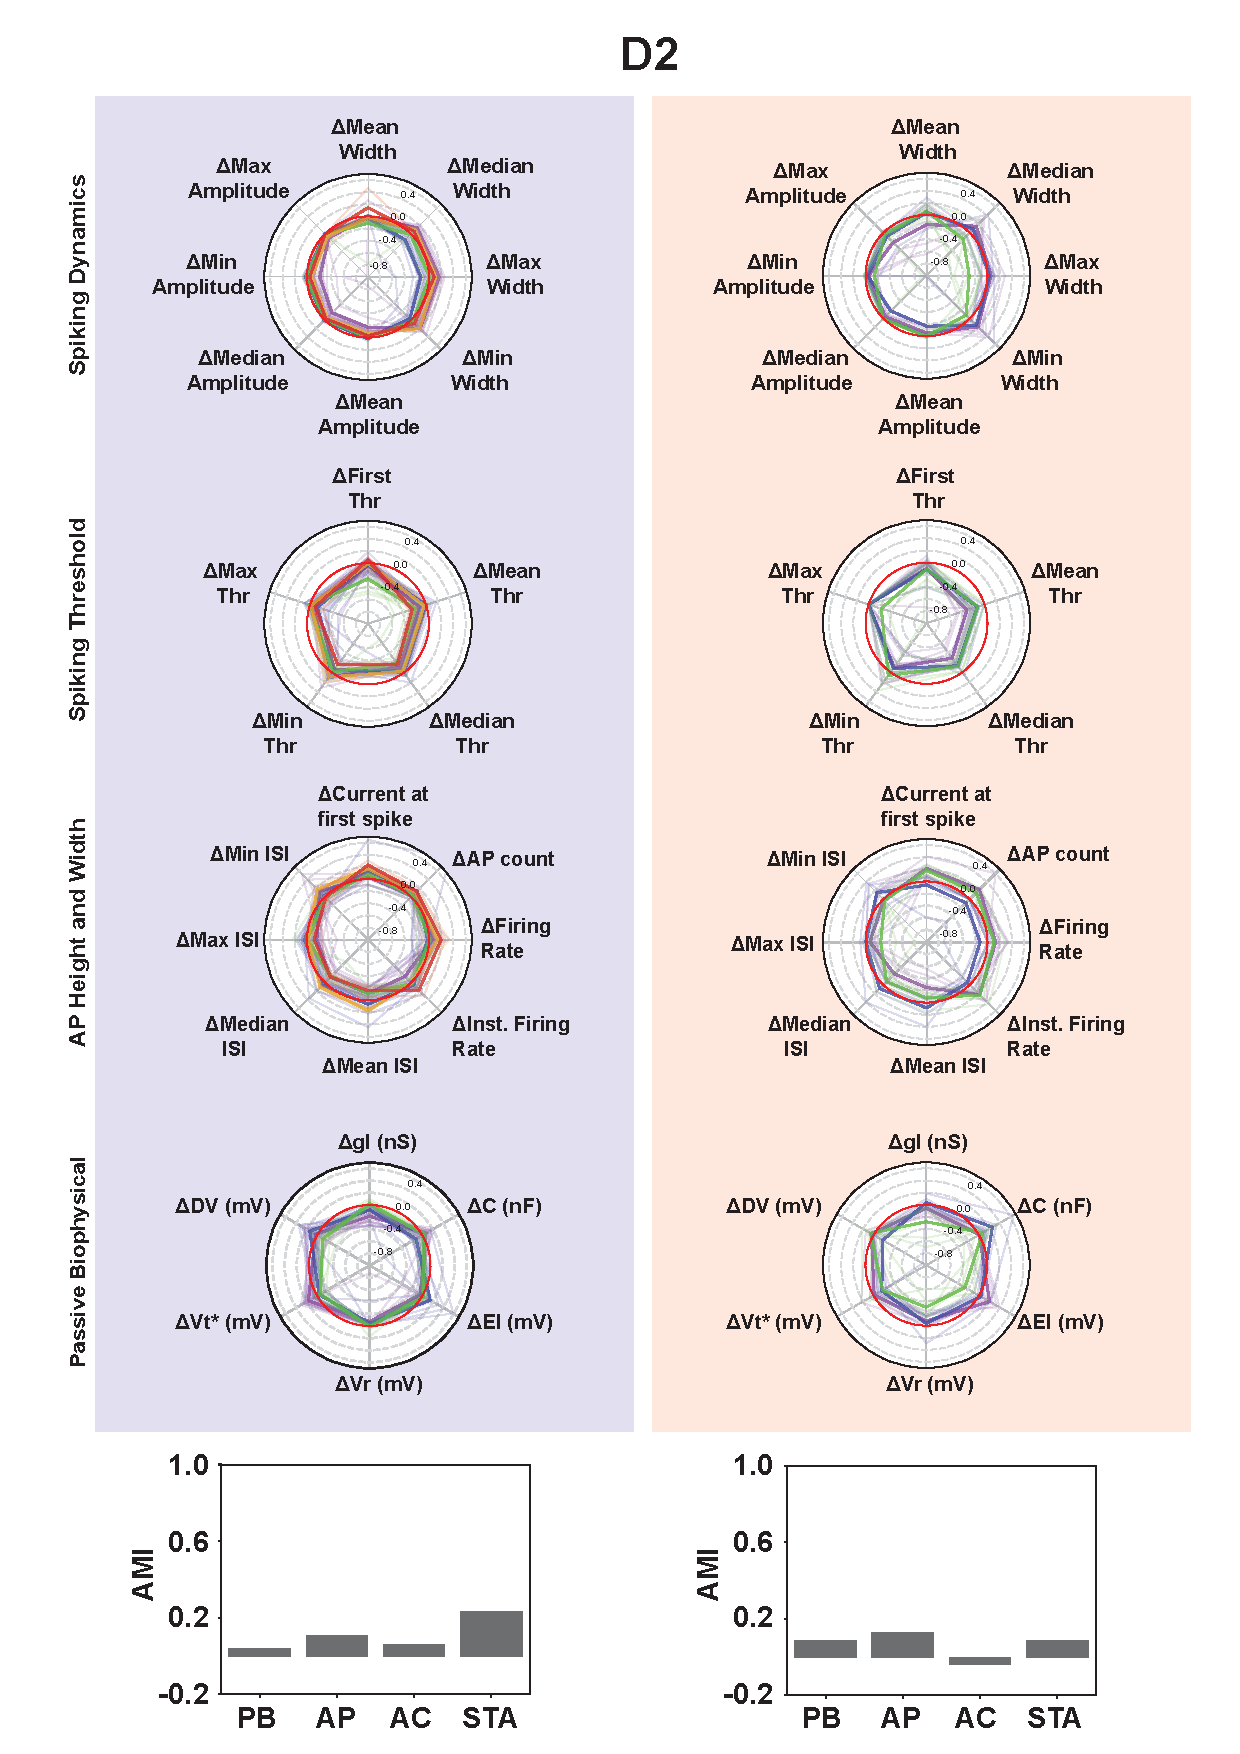
\includegraphics[width=0.9\linewidth]{Figures/Ch_3/Appendix8.pdf}
      \caption{\textbf{Clustering based on differences between control and D2 for action potential and passive biophysical attributes reveals subgroups of neurons getting modulated differently as a result of D2-R activation.}}
    \label{fig:S8}
\end{figure}

\begin{figure}
The polar plots show the clusters based on difference values between D2 and aCSF trials for action potential (subdivided into spiking dynamics, spiking threshold and AP height and width) and passive biophysical properties for both, excitatory (red background) and inhibitory (blue background). Each neuron is represented with a thin line and Coloured with their respective cluster label. The mean for each cluster is represented with a thick line. The histogram at the bottom shows the AMI score between cluster labels using aCSF trials and the cluster labels based on difference between D2 and aCSF trials.   
\end{figure}

\clearpage
\newpage

\begin{figure}
    \centering
    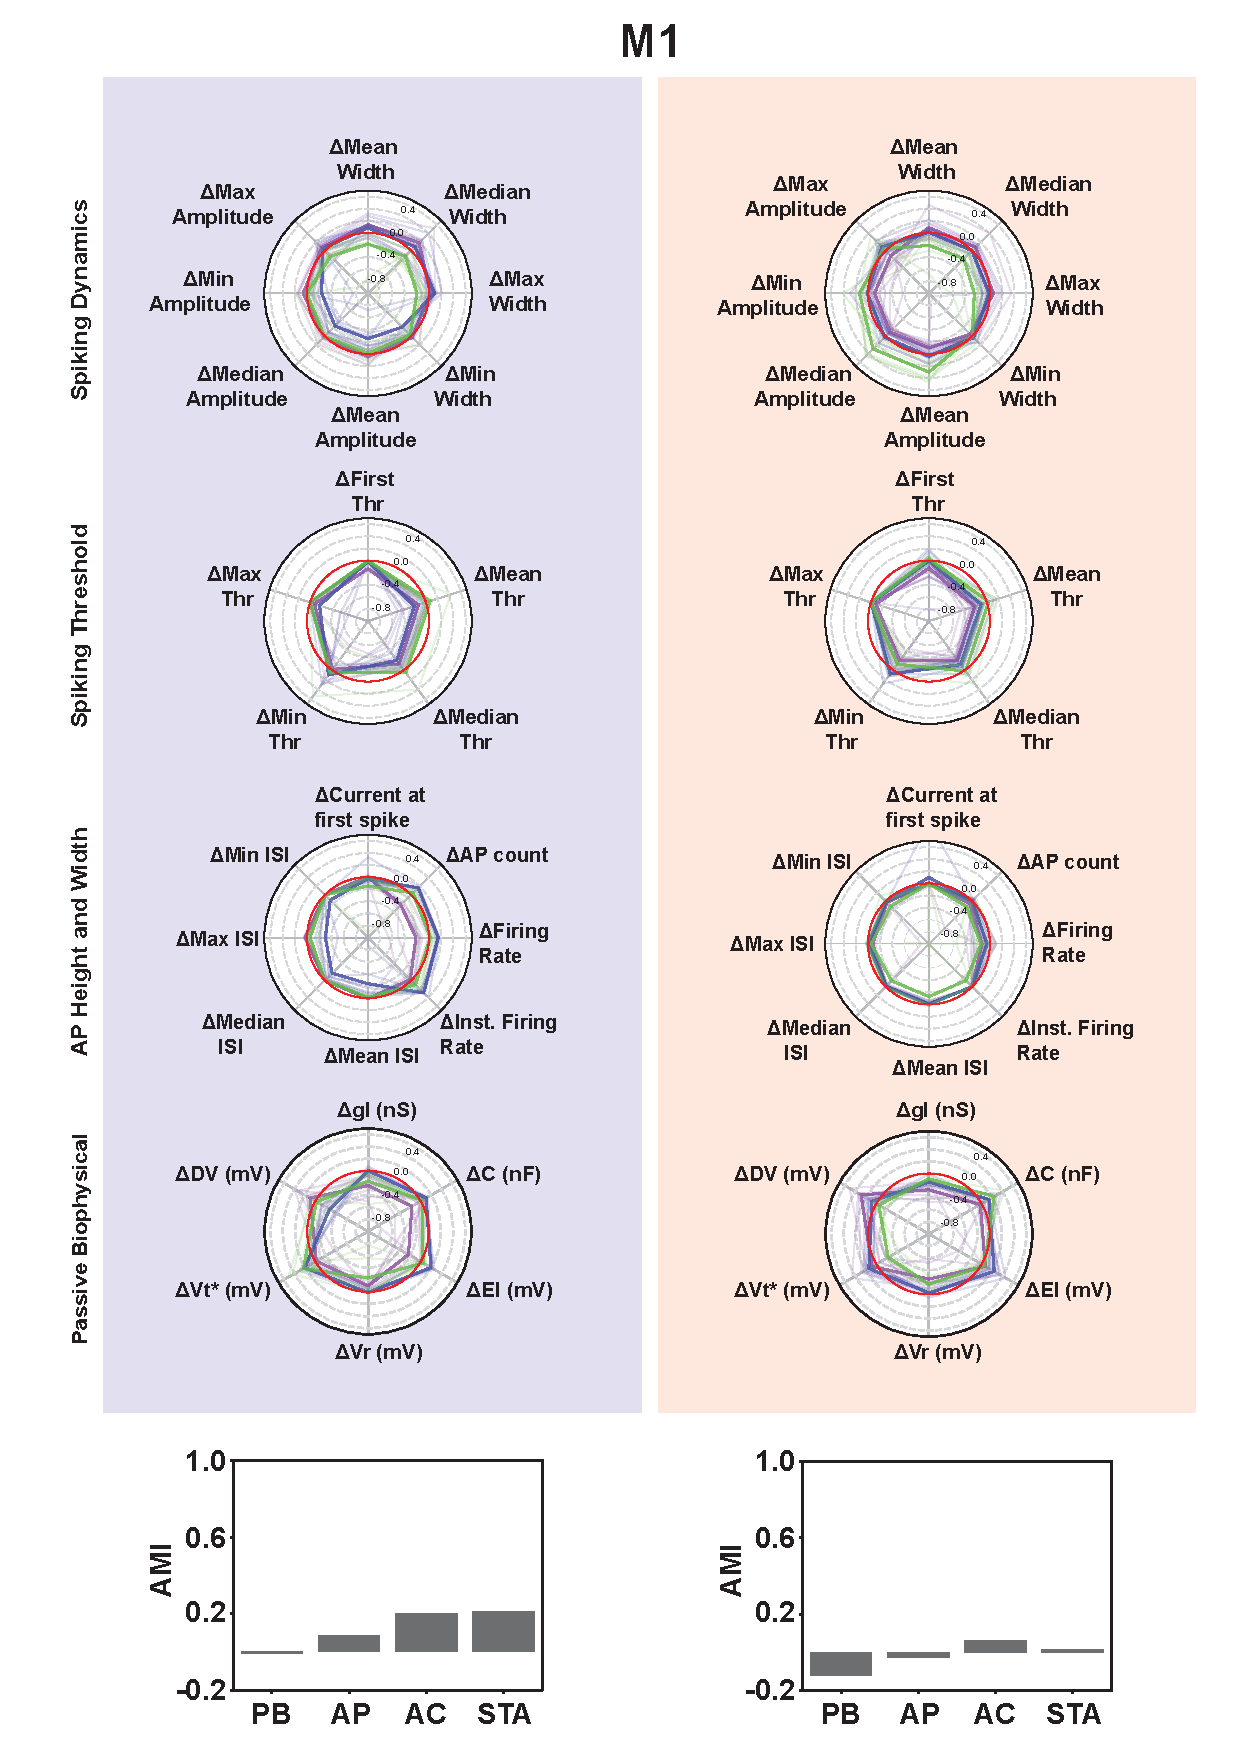
\includegraphics[width=0.9\linewidth]{Figures/Ch_3/Appendix9.pdf}
    \caption{\textbf{Clustering based on differences between control and M1 for action potential and passive biophysical attributes reveals subgroups of neurons getting modulated differently as a result of M1-R activation.}}
    \label{fig:S9}
\end{figure}


\newpage


\begin{figure}The polar plots show the clusters based on difference values between M1 and aCSF trials for action potential (subdivided into spiking dynamics, spiking threshold and AP height and width) and passive biophysical properties for both, excitatory (red background) and inhibitory (blue background). Each neuron is represented with a thin line and Coloured with their respective cluster label. The mean for each cluster is represented with a thick line. The histogram at the bottom shows the AMI score between cluster labels using aCSF trials and the cluster labels based on difference between M1 and aCSF trials.   
\end{figure}
\clearpage
\newpage
\begin{figure}
    \centering
    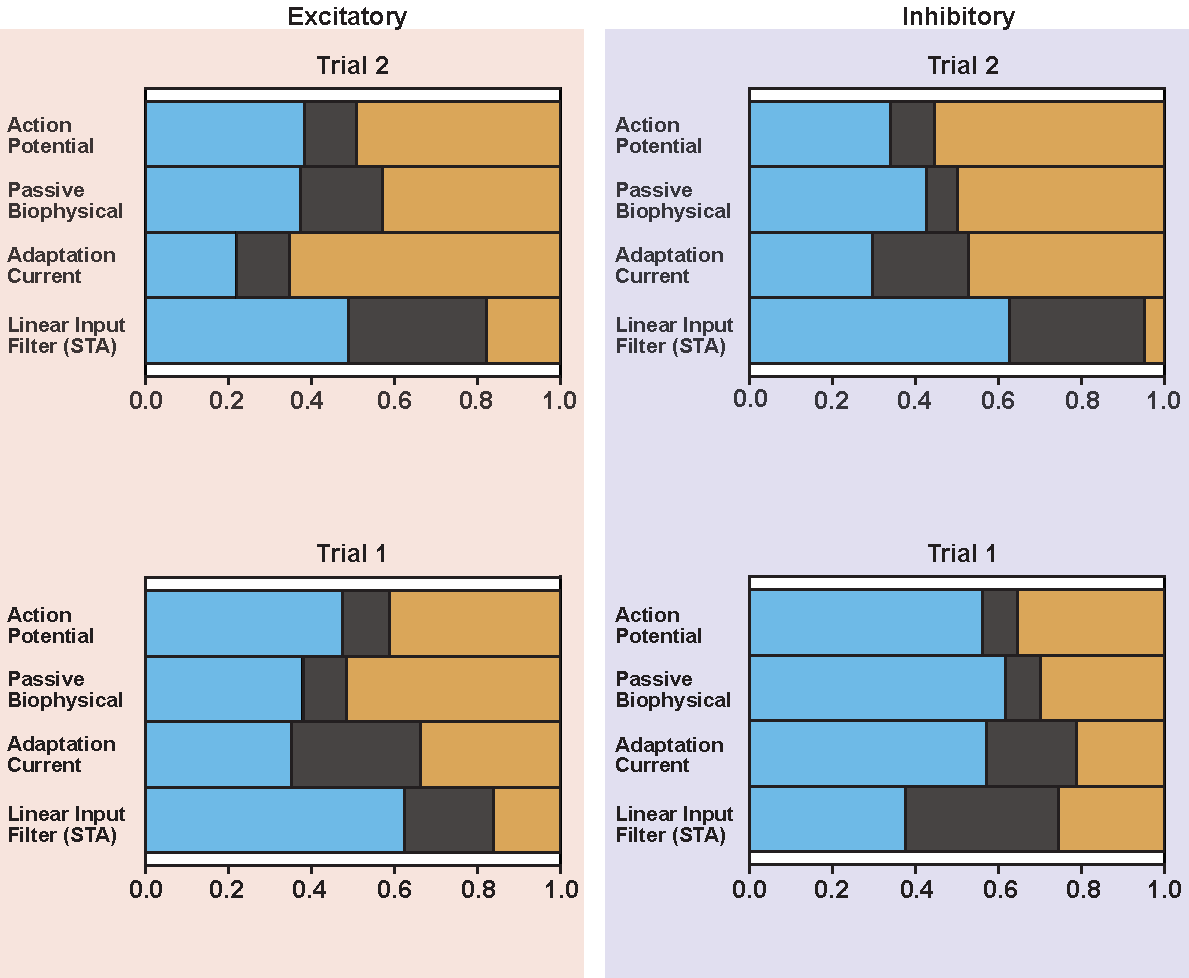
\includegraphics[width=0.9\linewidth]{Figures/Ch_3/Appendix10.pdf}
    \caption{\textbf{MCFA for 1st and 2nd aCSF trials.}}
    \label{fig:S10}
\end{figure}
\clearpage

\newpage

\begin{figure}
    \centering
    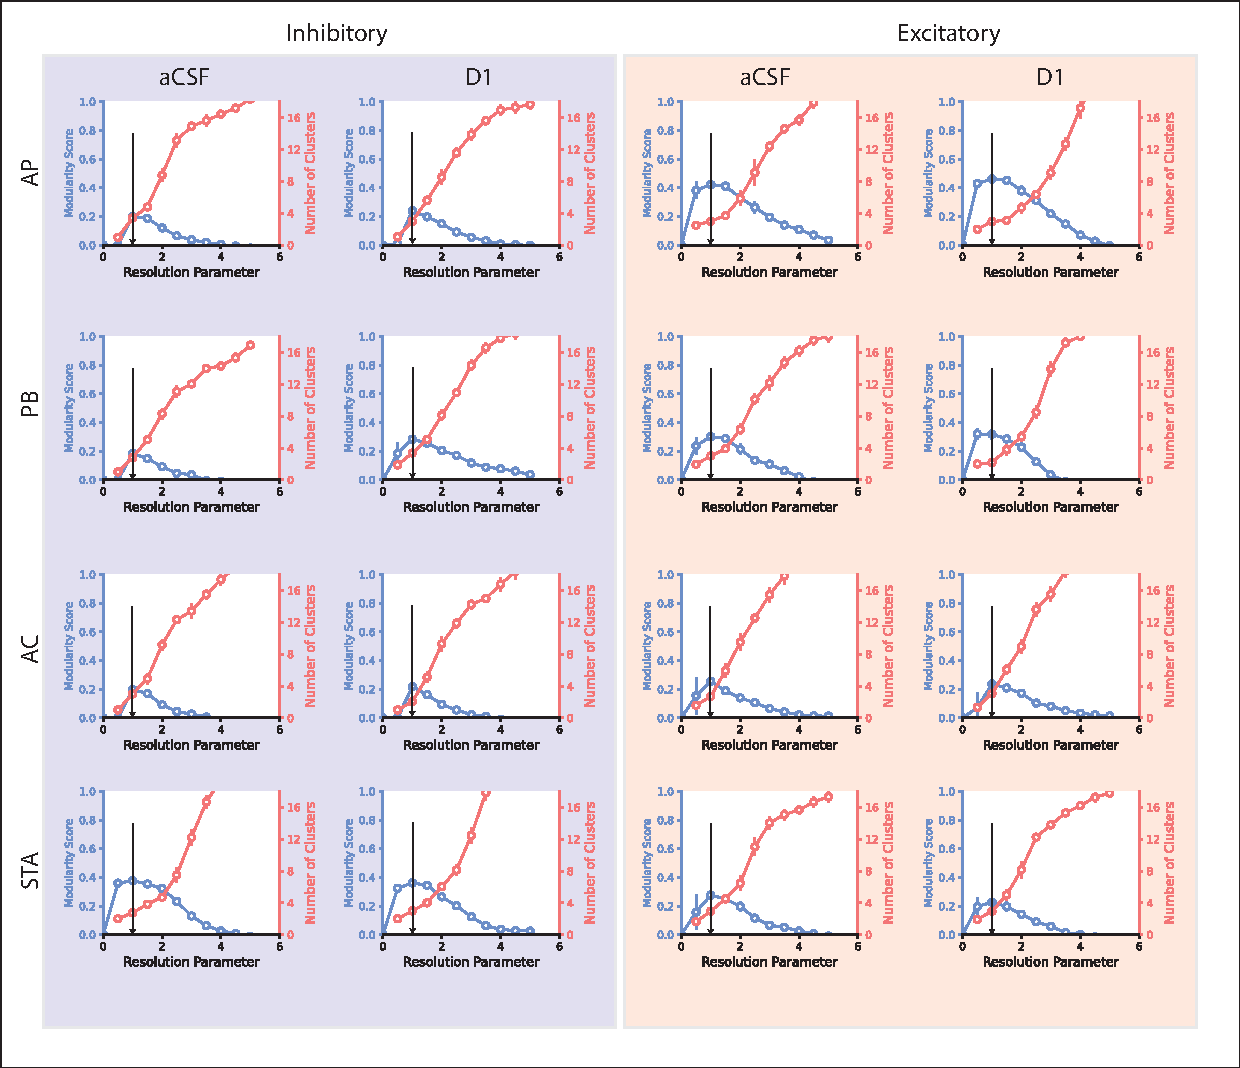
\includegraphics[width=\linewidth]{Figures/Ch_3/Appendix11.pdf}
    \caption{\textbf{Stability of clusters over a range of resolution parameters and the corresponding number of clusters for D1} The plot shows the modularity score for each resolution parameter and the corresponding number of clusters. The selected resolution parameter is marked with the black arrow, this corresponds to the highest modularity score.  }
    \label{fig:stability_d1}
\end{figure}
\clearpage

\begin{figure}
    \centering
    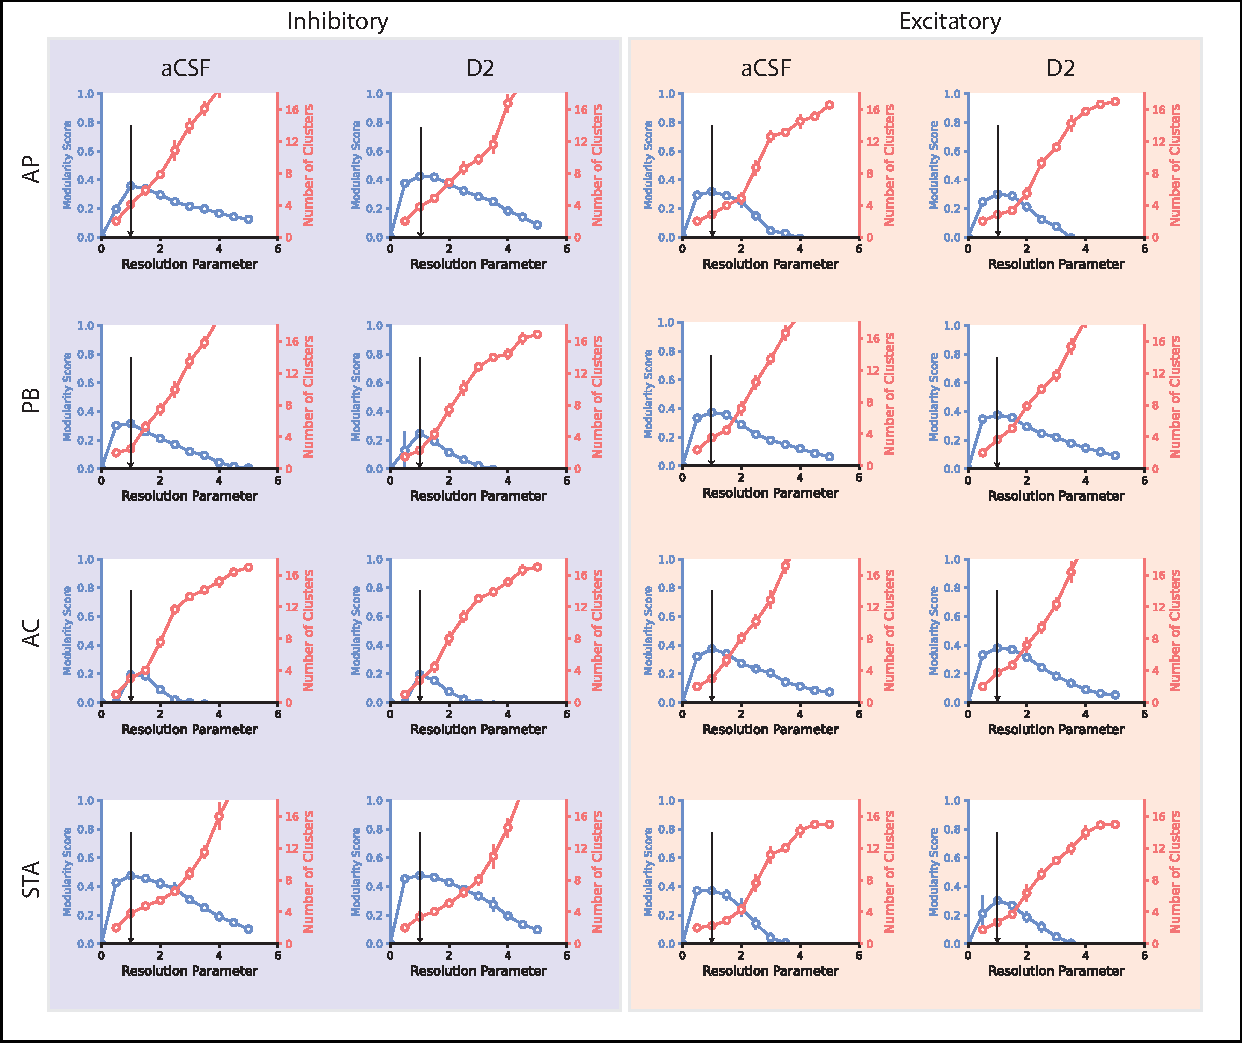
\includegraphics[width=\linewidth]{Figures/Ch_3/Appendix12.pdf}
    \caption{\textbf{Stability of clusters over a range of resolution parameters and the corresponding number of clusters for D2} The plot shows the modularity score for each resolution parameter and the corresponding number of clusters. The selected resolution parameter is marked with the black arrow, this corresponds to the highest modularity score.}
    \label{fig:stability_d2}
\end{figure}
\clearpage
\newpage

\begin{figure}
    \centering
    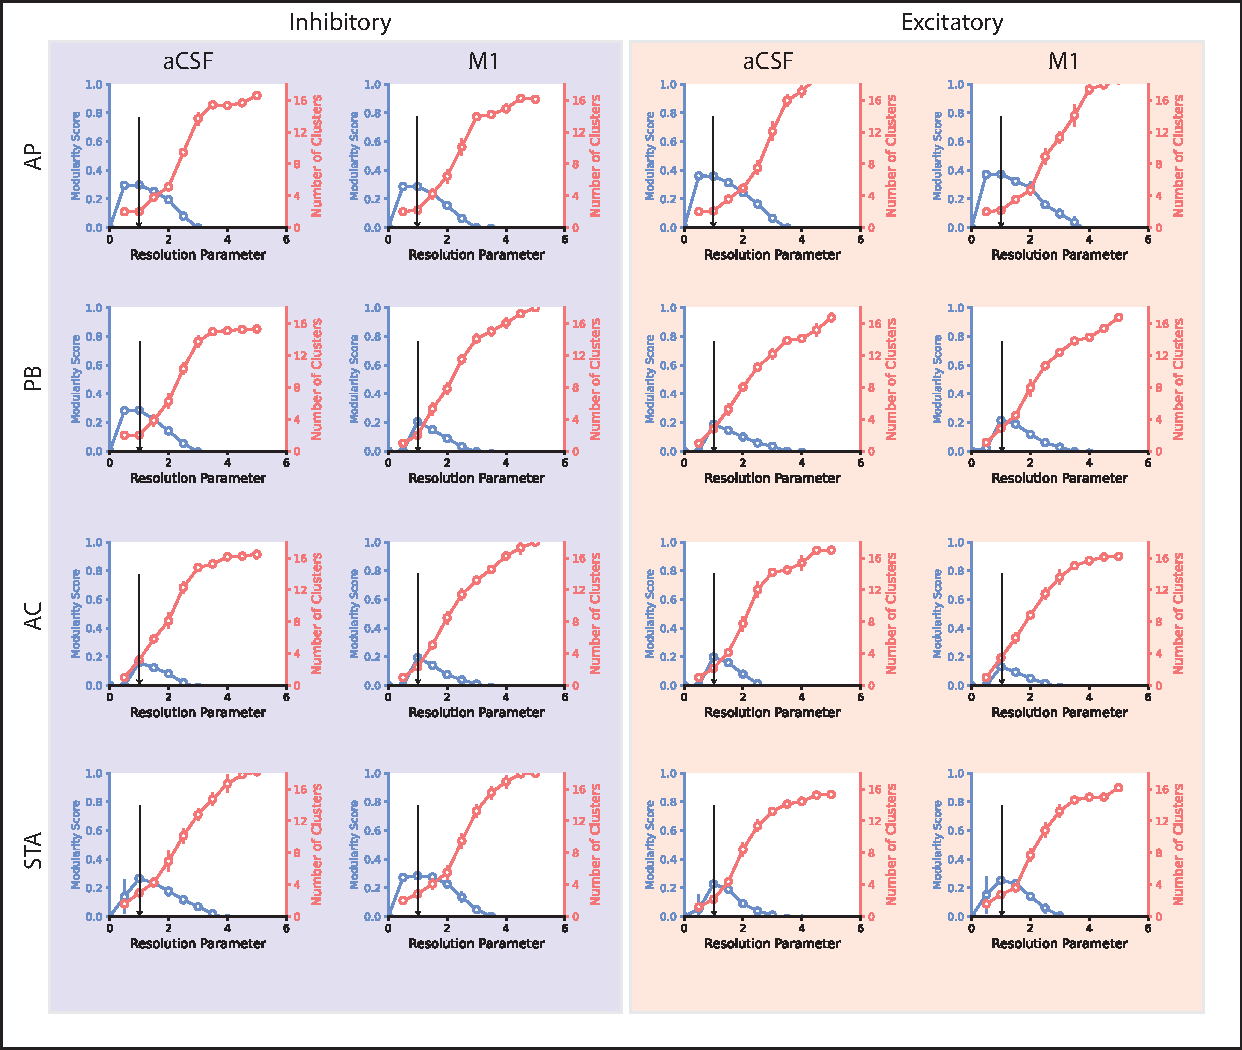
\includegraphics[width= \linewidth]{Figures/Ch_3/Appendix13.pdf}
    \caption{\textbf{Stability of clusters over a range of resolution parameters and the corresponding number of clusters for M1} The plot shows the modularity score for each resolution parameter and the corresponding number of clusters. The selected resolution parameter is marked with the black arrow, this corresponds to the highest modularity score.}
    \label{fig:stability_m1}
\end{figure}
\clearpage
\newpage
%%%%%%%%%%%%%%%% SUPPLEMENTARY TABLES %%%%%%%%%%%%%%%

\begin{table}[p]
\centering
\begin{tabular}{ccccc}
\hline
Condition         & Cell Type        & P‑value    & Statistic & Cohen’s \(d\)  \\
\hline 
D1–aCSF           & Inhibitory       & 0.019044   & 110       & –0.2409        \\
D1–aCSF           & Excitatory       & 0.104543   & 84        &  0.5385        \\
D2–aCSF           & Inhibitory       & 0.768005   & 87        & –0.0287        \\
D2–aCSF           & Excitatory       & 0.012016   & 225       &  0.3053        \\
M1–aCSF           & Inhibitory       & 0.523511   & 106       & –0.1181        \\
M1–aCSF           & Excitatory       & 0.002022   & 22        &  0.4790        \\
aCSF$_1$–aCSF$_2$ & Inhibitory       & 0.205410   & 170       & –0.3161        \\
aCSF$_1$–aCSF$_2$ & Excitatory       & 0.000111   & 340       &  0.3231        \\
\hline
\end{tabular}
\caption{Statistical comparison of fractional information (FI) changes under receptor activation.}
\label{tab:table1}
\end{table}
\clearpage
\newpage
%------------------------D1 ---------------------------------------------
% \newpage
    \begin{table}[p]
    \centering
    \begin{tabular}{llclllll}
        \hline
        Attribute & Variance type & aCSF &  D1 & D2 & M1 \\% 
        \hline
        AP  & Private   &  16.7742 (+/- 11.11)  & \textcolor{red}{0.0062}       & \textcolor{red}{0.1991}     &  \textcolor{red}{1.18E-03}     \\
        AP  & Shared    &  30.8543 (+/- 13.21)  & \textcolor{blue}{41.0578}     & \textcolor{blue}{55.0319}   &  \textcolor{blue}{66.0431}     \\
        AP  & Residual  &  52.3714 (+/- 12.18)  & \textcolor{blue}{58.9360}     & \textcolor{red}{44.7689}    &  \textcolor{red}{33.9556}      \\
        PB  & Private   &  18.5046 (+/- 13.50)  & \textcolor{red}{10.4084}      & \textcolor{red}{14.4461}    &  \textcolor{blue}{29.4316}      \\
        PB  & Shared    &  35.2320 (+/- 15.97)  & \textcolor{blue}{49.5931}     & \textcolor{red}{22.2190}    &  \textcolor{red}{26.3528}      \\
        PB  & Residual  &  46.2633 (+/- 15.84)  & \textcolor{red}{39.9985}      & \textcolor{blue}{63.2628}   &  \textcolor{red}{44.2155}      \\
        AC  & Private   &  18.0218 (+/- 17.14)  & \textcolor{red}{5.7216}       & \textcolor{red}{16.8436}    &  \textcolor{red}{10.3262}      \\
        AC  & Shared    &  15.8369 (+/- 11.35)  & \textcolor{red}{6.9056}       & \textcolor{blue}{30.6685}   &  \textcolor{blue}{35.0802}     \\
        AC  & Residual  &  66.1412 (+/- 21.22)  & \textcolor{blue}{87.3728}     & \textcolor{red}{44.7689}   &  \textcolor{red}{54.5935}     \\
        STA & Private   &  57.7380 (+/- 24.75)  & \textcolor{blue}{73.9663}     & \textcolor{blue}{71.2200}   &  \textcolor{red}{2.8344}       \\
        STA & Shared    &  23.6072 (+/- 19.86)  & \textcolor{red}{9.5260}       & \textcolor{red}{18.0047}   &  \textcolor{red}{6.9094}       \\
        STA & Residual  &  18.6546 (+/- 18.49)  & \textcolor{red}{16.5077}      & \textcolor{red}{10.7753}    &  \textcolor{blue}{90.2561}      \\     
        \hline
    \end{tabular}
    \caption{\textbf{Excitatory MCFA results}. Values that are reduced compared to bootstrapped aCSF are colored in red and values that are increased compared to aCSF are colored in blue. }
    \label{tab:specific_values_exc}
    \end{table}
\clearpage    
\newpage
\begin{table}[!htpb]
    \centering
    \begin{tabular}{llclllll}
        \hline
        Attribute & Variance type  & aCSF &  D1 & D2 & M1  \\
        \hline
        AP  & Private   & 14.9272 (+/- 09.5664)   &  \textcolor{red}{0.8297}     &  \textcolor{red}{1.6361}    &  \textcolor{red}{6.3213}       \\ 
        AP  & Shared    & 33.3099 (+/- 12.0733)   &  \textcolor{red}{32.3923}    &  \textcolor{red}{24.0248}   &  \textcolor{blue}{46.7960}    \\
        AP  & Residual  & 51.7627 (+/- 10.2972)   &  \textcolor{blue}{66.7777}   &  \textcolor{blue}{74.3390}  &  \textcolor{red}{46.8826}     \\
        PB  & Private   & 13.1228 (+/- 10.4672)   &  \textcolor{red}{3.9880}     &  \textcolor{red}{11.2795}   &  \textcolor{blue}{18.8554}    \\
        PB  & Shared    & 33.4015 (+/- 14.8031)   &  \textcolor{red}{25.2733}    &  \textcolor{blue}{53.6689}  &  \textcolor{blue}{51.5773}    \\
        PB  & Residual  & 53.4755 (+/- 15.0643)   &  \textcolor{blue}{70.7389}   &  \textcolor{red}{35.0514}   &  \textcolor{red}{29.5671}     \\
        AC  & Private   & 22.7058 (+/- 16.5534)   &  \textcolor{red}{11.6295}    &  \textcolor{blue}{26.3594}  &  \textcolor{blue}{50.6683}     \\
        AC  & Shared    & 26.9763 (+/- 14.6503)   &  \textcolor{blue}{44.4749}   &  \textcolor{blue}{38.9088}  &  \textcolor{red}{22.8306}    \\
        AC  & Residual  & 50.3177 (+/- 21.2265)   &  \textcolor{red}{43.8957}    &  \textcolor{red}{35.0514}   &  \textcolor{red}{26.5009}    \\
        STA & Private   & 55.1458 (+/- 25.8562)   &  \textcolor{red}{48.3895}    &  \textcolor{red}{21.5490}   &  \textcolor{red}{36.3625}    \\
        STA & Shared    & 23.6595 (+/- 17.2281)   &  \textcolor{blue}{46.2345}   &  \textcolor{blue}{66.6929}  &  \textcolor{blue}{54.3020}     \\   
        STA & Residual  & 21.1946 (+/- 21.2975)   &  \textcolor{red}{5.3761}     &  \textcolor{red}{11.7580}   &  \textcolor{red}{9.3353}       \\        
        \hline
    \end{tabular}
    \caption{\textbf{Inhibitory MCFA results}. Values that are reduced compared to bootstrapped aCSF are colored in red and values that are increased compared to aCSF are colored in blue. }
    \label{tab:specific_values_inh}
    \end{table}

\clearpage    
\newpage
    
    
\begin{table}[!htpb]
    \centering
    \begin{tabular}{llcc}
    \hline
    Attribute & Variance type  & Variance 1st Trial & Variance 2nd Trial \\
    \hline
    AP 	    & Private  &  11.2873 (+/- 11.81)	&\textcolor{blue}{12.4735 (+/- 08.39)}\\
    AP 	    & Shared   &  47.5009 (+/- 15.28)	&\textcolor{red}{38.4021 (+/- 10.44)}\\
    AP 	    & Residual &  41.2118 (+/- 10.25)	&\textcolor{blue}{49.1244 (+/- 08.84)}\\
    PB 	    & Private  &  10.3859 (+/- 08.94)	&\textcolor{blue}{19.9091 (+/- 12.32)}\\
    PB 	    & Shared   &  38.0565 (+/- 14.78)	&\textcolor{red}{37.3036 (+/- 14.24)}\\
    PB 	    & Residual &  51.5576 (+/- 18.05)	&\textcolor{red}{42.7873 (+/- 13.55)}\\
    AC 	    & Private  &  31.0247 (+/- 16.07)	&\textcolor{red}{12.7529 (+/- 09.86)}\\
    AC 	    & Shared   &  35.2139 (+/- 15.73)	&\textcolor{red}{22.0695 (+/- 11.62)}\\
    AC 	    & Residual &  33.7614 (+/- 14.71)	&\textcolor{blue}{65.1776 (+/- 16.40)}\\
    STA 	& Private  &  21.4966 (+/- 16.40)	&\textcolor{blue}{33.4581 (+/- 23.06)}\\
    STA 	& Shared   &  62.5138 (+/- 17.43)	&\textcolor{red}{48.8704 (+/- 25.72)}\\
    STA 	& Residual &  15.9897 (+/- 08.43)	&\textcolor{blue}{17.6716 (+/- 15.15)}\\
    \hline
    \end{tabular}
    \caption{\textbf{Excitatory MCFA results for second aCSF trial}. Values that are reduced compared to bootstrapped aCSF trial 1 are colored in red and values that are increased compared to aCSF trial 1 are colored in blue.}
    \label{tab:specific_values_exc_acsf}
    \end{table}
\clearpage    
\newpage    
\begin{table}[!htpb]
    \centering
    \begin{tabular}{llcc}
    \hline
    Attribute & Variance type  & Variance 1st Trial & Variance 2nd Trial \\
    \hline
    AP 	    & Private  &  08.4805 (+/- 07.68)  &	\textcolor{blue}{10.5232 (+/- 07.13)}\\
    AP 	    & Shared   &  56.1049 (+/- 11.24)  &	\textcolor{red}{33.9479 (+/- 17.05)} \\
    AP 	    & Residual &  35.4145 (+/- 07.97)  & 	\textcolor{blue}{55.5289 (+/- 18.73)}\\
    PB 	    & Private  &  08.3097 (+/- 06.94)  &	\textcolor{red}{07.4436 (+/- 09.55)}\\
    PB 	    & Shared   &  61.6040 (+/- 12.22)  &	\textcolor{red}{42.5329 (+/- 16.00)}\\
    PB 	    & Residual &  30.0864 (+/- 09.39)  & 	\textcolor{blue}{50.0235 (+/- 15.53)}\\
    AC 	    & Private  &  21.8111 (+/- 10.96)  &	\textcolor{blue}{23.1401 (+/- 15.18)}\\
    AC 	    & Shared   &  56.9907 (+/- 12.05)  &	\textcolor{red}{29.6210 (+/- 10.40)}\\
    AC 	    & Residual &  21.1982 (+/- 09.24)  & 	\textcolor{blue}{47.2389 (+/- 15.30)}\\
    STA 	& Private  &  36.8157 (+/- 23.86)  &	\textcolor{red}{32.6709 (+/- 21.86)}\\
    STA 	& Shared   &  37.5418 (+/- 17.49)  &	\textcolor{blue}{62.5230 (+/- 22.45)}\\
    STA 	& Residual &  25.6425 (+/- 22.69)   & 	\textcolor{red}{04.806 (+/- 02.85)}\\
    \hline
    \end{tabular}
    \caption{\textbf{Inhibitory MCFA results for second aCSF trial}. Values that are reduced compared to bootstrapped aCSF trial 1 are colored in red and values that are increased compared to aCSF trial 1 are colored in blue. }
    \label{tab:specific_values_inh_acsf}
    \end{table}


\newpage
\begin{spacing}{1.0} % Set the line spacing to single spacing
\fontsize{8pt}{8pt}\selectfont
\bibliographystyle{apalike} %%%%Changed
\renewcommand{\bibname}{References}
\bibliography{All_bibtex} %%%%Changed
\end{spacing}
% \printbibliography
% %-------------------------------------------
\chapter{Appendices}
\AddToShipoutPictureBG*{%
  \AtPageLowerLeft{%
    \begin{tikzpicture}[remember picture, overlay]
      \node[inner sep=0] at (current page.center) {\includegraphics[width=\paperwidth, height=\paperheight]{Figures/cover_bg.pdf}};
    \end{tikzpicture}
  }
}
\vspace{3cm}
{\Centering Nederlandse samenvatting \newline Research data management statement \newline Outreach activities \newline Failures \newline Acknowledgements \newline Curriculum Vitae \newline Donders Graduate School \newline} 
% \ChapFrame
\thispagestyle{empty}


\fancyhf{}
\fancyhead[c]{Chapter 8. Appendices}% <- added
\fancyfoot[R]{\thepage\ifodd\value{page}\else\hfill\fi}
%\fancyhead[L]{\ifodd\value{page}\relax\else\hfill\fi Ch \thechapter}
%\renewcommand\headrulewidth{0pt}% default ist .4pt
\renewcommand{\plainheadrulewidth}{.4pt}% default is 0pt

\section{Nederlandse samenvatting}
\tab Dit proefschrift bevat cross-sectionele en longitudinale onderzoeken die verbanden tussen voeding en gedrag onderzochten. Voor gedrag is er onder andere specifiek gekeken naar executieve functies en inhibitievermogen. Executieve functies zijn belangrijke processen die plaatsvinden in het brein om doelgerichte handelingen zo efficiënt mogelijk uit te voeren. Hierbij kan men bijvoorbeeld denken aan het bakken van een taart: wanneer de oven wordt aangezet voordat het beslag wordt gemaakt, dan is de oven al op temperatuur wanneer het beslag klaar is. Inhibitie, ofwel het vermogen om impulsen te beheersen, speelt een belangrijke rol in deze executieve functies.

De onderzochte verbanden in dit proefschrift reiken van het vroege leven tot de adolescentie. De darmbacterie-brein as, ofwel de communicatieroute tussen de darmbacteriën en het brein, is een belangrijk mechanisme dat de verwachte verbanden zou kunnen verklaren. Het eerste doel van dit proefschrift was om de relaties te onderzoeken tussen borstvoedingsfactoren en gedrag bij peuters. Het tweede doel was om de relaties te onderzoeken tussen darmbacteriën en gedrag bij peuters. Het derde doel was om de rol van de kwaliteit van de zorg van de moeder, meerdere keren gemeten tussen geboorte van het kind en de adolescentie, in het voedingsgedrag van adolescenten te onderzoeken.

In \textbf{hoofdstuk 2} is onderzocht of de lengte van de borstvoedingsperiode, ofwel borstvoedingsduur, het inhibitievermogen van een peuter voorspelt. Vervolgens is onderzocht of de dieetkwaliteit van een peuter een tussenrol speelt in deze voorspelling. In de eerste drie jaren na de bevalling, hebben moeders de borstvoedingsduur bijgehouden. Op driejarige leeftijd is het inhibitievermogen van het kind in kaart gebracht met behulp van vier verschillende gedragstaken. Ook zijn er vragenlijsten bij beide ouders afgenomen om het gedrag van het kind in kaart te brengen. De voedingsvragenlijst over de voedingsinname van de peuters is ingevuld door één van de ouders. Er is geen bewijs gevonden voor een verband tussen borstvoedingsduur en inhibitievermogen. Resultaten van voorgaand onderzoek op dit onderwerp liepen al uiteen, waarschijnlijk onder meer door het gebruik van verschillende meetmethoden. Net als voorgaand onderzoek wees ons onderzoek wel uit dat langere borstvoedingsduur een betere dieetkwaliteit van de peuters voorspelt. Het is echter niet duidelijk wat het mechanisme achter dit verband is. Hoe belangrijk moeders gezonde voeding vinden is mogelijk een belangrijke speler in dit verband.

In \textbf{hoofdstuk 3} is er onderzocht of humane melk oligosachariden (HMOs), de executieve functies en het inhibitievermogen van peuters voorspelt. HMOs zijn complexe suikers die aanwezig zijn in moedermelk. Moeders hebben hiervoor op twee, zes en 12 weken een kleine hoeveelheid melk verzameld. Van deze melk is de HMO-samenstelling geanalyseerd. Dezelfde meetmethoden benoemd in hoofdstuk 2 zijn gebruikt om executieve functies en inhibitie bij de peuters te meten. Resultaten lieten zien dat hoge niveaus van gefucosyleerde HMOs gerelateerd zijn aan betere executieve functies bij peuters. Er is geen bewijs gevonden voor een verband tussen gesialyleerde HMOs en executieve functies bij peuters. Onze resultaten wat betreft gefucosyleerde HMOs komen overeen met voorgaand soortgelijk onderzoek in dieren en mensen. Onze resultaten over gesialyleerde HMOs komen gedeeltelijk overeen met soortgelijke studies. Dit komt omdat er uiteenlopende resultaten zijn gevonden in voorgaand onderzoek. Deze verschillen zijn te verklaren door het gebruik van verschillende onderzoeksmethoden en de leeftijden waarop het gedrag van de kinderen is gemeten. Dit is het eerste onderzoek bij mensen dat HMOs heeft gemeten op drie tijdspunten binnen de eerste drie maanden. Replicatie van dit onderzoek is daarom belangrijk.

In \textbf{hoofdstuk 4} zijn de relaties tussen darmbacteriën en executieve functies (inclusief inhibitievermogen) van peuters onderzocht. Dezelfde meetmethoden benoemd in hoofdstuk 2 zijn gebruikt om de executieve functies en inhibitie te meten. Op twee, zes en 12 weken en op één en drie jaar, is de compositie van de darmbacteriën van het kind geanalyseerd. Er zijn verbanden gevonden tussen hogere niveaus van \textit{Streptococcus}, [\textit{Ruminococcus}] \textit{Torques} groep, \textit{Clostridium sensu stricto} 1, \textit{Intestinibacter}, en \textit{Halomonas} en verminderde executieve functies bij peuters. Een hoger niveau van \textit{Bacteroides}, \textit{Parabacteroides}, \textit{Ruminococcus} 2, en \textit{Blautia} en een hogere diversiteit aan verschillende soorten darmbacteriën bleken  gerelateerd aan betere executieve functies. Hogere niveaus van \textit{Bacteroides}, \textit{Ruminococcaceae} UCG-013 en \textit{Veillonella} voorspelden betere inhibitievermogen. Hogere niveaus van \textit{Subdoligranulum}, \textit{Lachnospiraceae} NK4A136, \textit{Anaerostipes}, \textit{Sutterella} en \textit{Coprococcus} 3 voorspelden verminderde inhibitievermogen in peuters. Resultaten van voorgaande onderzoeken overlappen gedeeltelijk met de bevindingen van dit proefschrift. Zo heeft eerder onderzoek ook een verband gevonden tussen \textit{Bacteroides} en beter inhibitievermogen. Er zijn echter ook verbanden gevonden die niet in voorgaand onderzoek naar voren kwamen. Verschillen tussen de resultaten van ons onderzoek en eerder onderzoek komt mede doordat er sprake is van verschillende leeftijden en gedragsmaten die zijn onderzocht. Meer (replicatie) onderzoek is nodig om de gevonden relaties te bevestigen en de bewijskracht te versterken.  

In \textbf{hoofdstuk 5} zijn de voorspellers van de kwaliteit van voeding van adolescenten onderzocht. Kwaliteit van zorg van de moeder is onderzocht op de kinderleeftijden van vijf weken, 12 maanden, twee-en-een-half jaar, 10 jaar en 14 jaar. Dit is onderzocht aan de hand van video's van interacties tussen moeder en kind die door onafhankelijke beoordelaars scores hebben gekregen. Voedingsinname en emotie-eten van adolescenten is middels zelfrapportage verzameld. Verder is het inhibitievermogen van de adolescent gemeten met behulp van drie gedragstaken en een vragenlijst die is ingevuld door de moeder. Er is geen bewijs gevonden voor maternale zorgkwaliteit en inhibitievermogen of dieetkwaliteit. Wel is er bewijs gevonden voor een verband tussen betere inhibitievermogen en betere dieetkwaliteit bij adolescenten. Toekomstig onderzoek zou (zelf)rapportage en objectieve observaties moeten combineren om een beter beeld te krijgen over kwaliteit van de zorg van moeders (en partners) en hoe dat relateert aan het gedrag van adolescenten (voedingsinname en inhibitievermogen). Langlopende en experimentele onderzoeken zijn nodig om de richting van de verbanden te achterhalen.  

Samenvattend, specifieke suikers in moedermelk en bepaalde darmbacteriën voorspellen betere executieve functies bij peuters. Tevens is er een verband gevonden tussen het inhibitievermogen en de dieetkwaliteit van een adolescent. Ondanks dat deze bevindingen geen oorzakelijke verbanden kunnen aantonen, wijzen de resultaten erop dat voeding in het vroege leven en de darmbacteriën mogelijk een rol spelen in de executieve functies en het inhibitievermogen van peuters. Daarnaast suggereren de resultaten dat er samenspel is tussen inhibitievermogen en voedingsinname tijdens adolescentie. 

\vspace{0.5cm}
\noindent Belangrijkste bevindingen van dit proefschrift:
\begin{itemize}
\item Langere borstvoedingsduur voorspelt niet het inhibitievermogen van een peuter, maar wel betere dieetkwaliteit van de peuter op de leeftijd van drie jaar.
\item Hogere concentraties van gefucosyleerde HMOs in moedermelk voorspellen betere executieve functies op peuterleeftijd.
\item We vonden geen bewijs voor een verband tussen gesialyleerde HMOs in moedermelk en executieve functies op peuterleeftijd.
\item Hogere niveaus van de darmbacterieën \textit{Streptococcus}, [\textit{Ruminococcus}] \textit{Torques} groep, \textit{Clostridium sensu stricto} 1, \textit{Intestinibacter}, en \textit{Halomonas} zijn gerelateerd aan verminderde executieve functies in peuters.
\item Hogere niveaus van de darmbacterieën \textit{Bacteroides}, \textit{Parabacteroides}, \textit{Ruminococcus} 2 en \textit{Blautia} en hogere diversiteit aan verschillende soorten darmbacteriën zijn gerelateerd aan betere executieve functies in peuters.
\item Hogere niveaus van de darmbacterieën \textit{Bacteroides}, \textit{Ruminococcaceae} UCG-013 en \textit{Veillonella} voorspellen beter inhibitievermogen in peuters. 
\item Hogere niveaus van de darmbacterieën \textit{Subdoligranulum}, \textit{Lachnospiraceae} NK4A136, \textit{Anaerostipes}, \textit{Sutterella} en \textit{Coprococcus} 3 voorspellen verminderd inhibitievermogen in peuters.
\item Beter inhibitievermogen van adolescenten is gerelateerd aan betere dieetkwaliteit.
\item Er is geen bewijs gevonden dat de zorgkwaliteit van de moeder tijdens de kindertijd de inhibitie en dieetkwaliteit van adolescenten voorspelt.
\end{itemize}

\fancyhf{}
\fancyhead[C]{Chapter 8. Appendices}% <- added
\fancyfoot[R]{\thepage\ifodd\value{page}\else\hfill\fi}
%\fancyhead[L]{\ifodd\value{page}\relax\else\hfill\fi Ch \thechapter}
%\renewcommand\headrulewidth{0pt}% default ist .4pt
\renewcommand{\plainheadrulewidth}{.4pt}% default is 0pt
\newpage
\begin{spacing}{1.5}

\section{Research Data Management Statement}

\subsection{Ethics}

\subsection{FAIR principles}

\subsubsection{1. Findable}

\subsubsection{2. Accessible} 

\subsubsection{3. Interoperable}

\subsubsection{4. Reusable}

\subsection{Privacy}
\end{spacing}


\clearpage
\fancyhf{}
\fancyhead[c]{Chapter 8. Appendices}% <- added
\fancyfoot[R]{\thepage\ifodd\value{page}\else\hfill\fi}
%\fancyhead[L]{\ifodd\value{page}\relax\else\hfill\fi Ch \thechapter}
%\renewcommand\headrulewidth{0pt}% default ist .4pt
\renewcommand{\plainheadrulewidth}{.4pt}% default is 0pt
\section{Outreach activities}
 
\section{Brain Bee}

During my PhD, I also dedicated significant efforts towards scientific outreach and teaching. I was part of the Dutch Brain Olympiad (Brain Bee) from 2021 until 2024, which a national level Olympiad for high school students, encouraging them towards Neuroscience and Artificial Intelligence. During this time I helped out the Computational neuroscience and AI team in developing study materials for the participants and I also part of the organizing team for the Nijmegen chapter.  I have summarized my contributions to the read below:  

\subsection{Genetic Algorithms (Chapter 2.4)}

In this chapter, I introduced Genetic Algorithms (GAs) as a biologically inspired computational technique rooted in evolutionary principles such as natural and sexual selection. The chapter educates readers on how GAs model adaptation by iteratively improving a population of candidate solutions to solve complex optimization problems. Through clear explanations and detailed step-wise descriptions, I provided readers with:

\subsubsection{Biological Foundations:}

I explained the fundamental biological concepts behind evolution, highlighting natural selection and sexual selection as mechanisms that shape species adaptation. This laid the groundwork for understanding how these principles inform computational algorithms.

\subsubsection{Algorithmic Steps and Mechanics:}

I clearly outlined the stages of a GA   from initializing a population, through selection, crossover (recombination), and mutation operators, culminating in termination upon convergence. This was supported by illustrative examples such as evolving binary strings, which concretely demonstrate how offspring solutions combine and mutate parental traits.

\subsubsection{Fitness Function Concept:}

Emphasizing the critical role of the fitness function, I described how it quantifies the quality of candidate solutions relative to the problem environment, guiding selection and evolution toward better solutions.

\subsubsection{Applications in Neuroscience:}

To connect theory with practice, I discussed real-world uses of GAs in neuroscience, such as fitting complex conductance-based neuron models to electrophysiological data and characterizing ion channel kinetics, emphasizing GAs' strength in handling high-dimensional parameter spaces.

\subsubsection{Limitations:}

I also covered computational constraints of genetic algorithms, including their expense in time and resources, occasional lack of guaranteed optimality, and sensitivity to implementation choices like selection criteria and mutation probabilities, providing readers with a balanced perspective.

\subsubsection{Educational Features:}

The chapter includes a flowchart to visualize the GA process, key terms for review, and pointers to further learning materials including interactive simulations and videos, making it accessible for learners preparing for neuroscience competitions or seeking foundational knowledge.

\subsection{AI and Neuroscience Applications Outside the Brain: Ethics and Impact (Chapter 2.5)}

This chapter presented a broad, interdisciplinary exploration of how insights from neuroscience and AI intersect in societal contexts beyond brain research, highlighting ethical considerations and future impacts:

\subsubsection{Real-World AI Applications:}

I detailed diverse societal domains where neuroscience-inspired AI is applied, such as neuromarketing using brain activity to predict consumer behavior, consciousness research that probes the neural basis of subjective experience, and sleep studies enhanced by AI analysis of brain signals.

\subsubsection{Neurotechnology and Neuro-Robotics:}

The chapter introduces next-generation technologies including neuro-robotics, where biological neural models guide autonomous robot behavior, and neuromorphic computing, aiming to build human-brain-like energy-efficient spiking neuron-based processors. This cutting-edge content situates the reader at the frontier of AI-neuroscience innovation.

\subsubsection{Ethical Challenges:}

Emphasizing the ethical dimension, I discussed critical concerns posed by neurotechnologies (e.g., unknown long-term impacts, regulatory gaps), privacy of brain data, the limitations and risks of lie detection via fMRI, cognitive enhancement through drugs, and pressing dilemmas such as the moral algorithms in autonomous vehicles and judicial predictive software highlighting societal risks of bias and fairness.

\subsubsection{Societal Impact and Sustainability:}

I highlighted the transformative impact of AI-driven automation on employment, the cognitive effects of digital systems on users, and the urgent need to address the growing energy footprint of computational infrastructures globally. This holistic perspective prepares the reader to think critically about the promises and perils of emerging technologies.

\subsubsection{Didactic Structure and Resources:}

The chapter integrates learning objectives guiding reader focus, defines specialized terminology, and points to references and further reading to encourage deeper inquiry into ethical AI and neuroscience's societal roles.

\subsubsection{Overall Contribution Impact}

My work brings conceptual clarity, scientific rigor, and ethical awareness to the reader, equipping learners with a detailed understanding of genetic algorithms a central evolutionary computation tool and a thoughtful exploration of AI \& neuroscience beyond the laboratory. By blending foundational science with real-world examples and interdisciplinary viewpoints, I contributed substantially to making complex topics approachable and relevant for the next generation of computational neuroscientists and AI researchers. Moreover, this endeavor taught me how to simplify complex topics to accessible to a laymen audience which is not at all an easy task. It was a fruitful and compelling experience overall. 

 
\newpage

\clearpage
\fancyhf{}
\fancyhead[c]{Chapter 8. Appendices}% <- added
\fancyfoot[R]{\thepage\ifodd\value{page}\else\hfill\fi}
%\fancyhead[L]{\ifodd\value{page}\relax\else\hfill\fi Ch \thechapter}
%\renewcommand\headrulewidth{0pt}% default ist .4pt
\renewcommand{\plainheadrulewidth}{.4pt}% default is 0pt
\section{Failures}

\newpage

\fancyhf{}
\fancyhead[C]{Chapter 8. Appendices}% <- added
\fancyfoot[R]{\thepage\ifodd\value{page}\else\hfill\fi}
%\fancyhead[L]{\ifodd\value{page}\relax\else\hfill\fi Ch \thechapter}
%\renewcommand\headrulewidth{0pt}% default ist .4pt
\renewcommand{\plainheadrulewidth}{.4pt}% default is 0pt
\newpage


\section{Acknowledgements}
\begin{spacing}{1.5}

\end{spacing}
\fancyhf{}
\fancyhead[C]{Chapter 8. Appendices}% <- added
\fancyfoot[R]{\thepage\ifodd\value{page}\else\hfill\fi}
%\fancyhead[L]{\ifodd\value{page}\relax\else\hfill\fi Ch \thechapter}

\section{Curriculum Vitae}

\begin{wrapfigure}{I}{0.45\textwidth}
    \vspace{-0.45cm}
    \hspace{0.35cm}
    \includegraphics[width=0.41\textwidth]{Figures/Profile picture.pdf}
\end{wrapfigure}

Yvonne Willemsen was born in Wageningen on December 6th, 1992. She obtained her Bachelor's degree of Nutrition and Dietetics, at the Hogeschool Arnhem en Nijmegen in Nijmegen, minoring in infant and child nutrition. To understand the science behind what was taught during her Bachelor's studies, she continued studying Nutrition and Health at Wageningen University \& Research, where she completed two specializations: Molecular Nutrition \& Toxicology and Nutritional Physiology \& Health Status. For both these specializations, her theses focused on toddler, and child nutrition. Within this Master's track, she also did her internship at TNO where she wrote a review on gut microbiota, antibiotics use in early life, and its relations with obesity development. All these previous experiences contributed to her growing interest in the interactions between gut microbiota, nutrition, and health. She was granted an ideal fitting PhD position at the Radboud University (RU) and the Radboudumc (RUMC) in Nijmegen. Under the supervision of Prof. dr. Carolina de Weerth (RUMC), Dr. Roseriet Beijers (RU) and Dr. Alejandro Arias Vásquez (RUMC), she conducted research on (early life) nutrition, gut microbiota, and behaviour as described in this thesis.

\fancyhf{}
\fancyhead[C]{Chapter 8. Appendices}% <- added
%\fancyhead[L]{\ifodd\value{page}\relax\else\hfill\fi Ch \thechapter}
\fancyfoot[R]{\thepage\ifodd\value{page}\else\hfill\fi}

%\renewcommand\headrulewidth{0pt}% default ist .4pt
\renewcommand{\plainheadrulewidth}{.4pt}% default is 0pt
\section{Donders Graduate School for Cognitive Neuroscience}
\begin{spacing}{1.5}
\tab For a successful research Institute, it is vital to train the next generation of young scientists. To achieve this goal, the Donders Institute for Brain, Cognition and Behaviour established the Donders Graduate School for Cognitive Neuroscience (DGCN), which was officially recognised as a national graduate school in 2009. The Graduate School covers training at both Master's and PhD level and provides an excellent educational context fully aligned with the research programme of the Donders Institute. 

The school successfully attracts highly talented national and international students in biology, physics, psycholinguistics, psychology, behavioral science, medicine and related disciplines. Selective admission and assessment centers guarantee the enrolment of the best and most motivated students.

The DGCN tracks the career of PhD graduates carefully. More than 50\% of PhD alumni show a continuation in academia with postdoc positions at top institutes worldwide, e.g., Stanford University, University of Oxford, University of Cambridge, UCL London, MPI Leipzig, Hanyang University in South Korea, NTNU Norway, University of Illinois, North Western University, Northeastern University in Boston, ETH Zürich, University of Vienna etc. Positions outside academia spread among the following sectors: specialists in a medical environment, mainly in genetics, geriatrics, psychiatry and neurology. Specialists in a psychological environment, e.g. as specialist in neuropsychology, psychological diagnostics or therapy. Positions in higher education as coordinators or lecturers. A smaller percentage enters business as research consultants, analysts or head of research and development. Fewer graduates  stay in a research environment as lab coordinators, technical support or policy advisors. Upcoming possibilities are positions in the IT sector and management position in pharmaceutical industry. In general, the PhDs graduates almost invariably continue with high-quality positions that play an important role in our knowledge economy.

For more information on the DGCN as well as past and upcoming defenses please visit: http://www.ru.nl/donders/graduate-school/phd/

\end{spacing}

\newpage
\thispagestyle{empty}
    \begin{tikzpicture}[remember picture, overlay]
      \node[inner sep=0] at (current page.center) {\includegraphics[width=\paperwidth, height=\paperheight]{Figures/cover_back_sign.pdf}};
    \end{tikzpicture}
\end{document}